\chapter{Стабилизация маятника: модальное управление}
\label{ch:chap3}

\section{Синтез регулятора по состоянию}

Синтезируем регулятор вида 
\begin{equation}
    u = Kx
\end{equation}
основываясь на линеаризованной модели (\ref{1_model_lin}). В ходе анализа математической модели было выяснено, что система является полностью управляемой и спектр системы $\sigma(A) = \{ 0,\, \,  0, \, \,  2.4165,\, \,  -2.4165\}$.


Для нахождения матрицы регулятора $K$ будем решать систему, содержающую уравнение Сильвестра

\begin{equation}
    \label{3_sil_reg}
    \begin{cases}
        AP -P \Gamma = BY\\
        K = -YP^{-1}
    \end{cases}
\end{equation}
Запишем условия существования решения $P$: $\sigma(A) \cap \sigma(\Gamma) = \emptyset$, $(A,B)$ -- управляема, $(Y, \Gamma)$ -- наблюдаема. Заметим, что второе условие выполнено. 

Учтем то, что порядок ненулевых коэффициентов матрицы $B$ примерно $10^{-3}$, в то время, как матрица $A$ содержит элементы порядка единиц. Это может потребовать больших коэффициентов $K$, постараемся подобрать желаемый спектр так, чтобы требуемое управление было минимальным необходимым для стабилизации системы.  Зададимся желаемым спектром замкнутой системы ближе к мнимой оси $\sigma (A+BK) = \{-0.3, \, \, -0.25, \, \, -0.2, \, \, -0.15 \}$. Запишем подходящие матрицы $\Gamma$ и $Y$

\begin{equation}
    \Gamma = \begin{bmatrix}
        -0.3 & 0 & 0 & 0\\
        0 & -0.25 & 0 & 0\\
        0 & 0 & -0.2 & 0\\
        0 & 0 & 0 & -0.15
    \end{bmatrix}, 
    Y = \begin{bmatrix}
        1 & 1 & 1 & 1
    \end{bmatrix}
\end{equation}

Проверим, что пара $(Y, \Gamma)$ -- наблюдаема: составим матрицу наблюдаемости и определим ее ранг

\begin{multline}
    V = \begin{bmatrix}
        Y\\ Y \Gamma \\ Y \Gamma^2 \\ Y \Gamma^3
    \end{bmatrix} = \begin{bmatrix}
        1&	1 &1&	1\\
-0.3&-0.25&-0.2&-0.15\\
0.09&	0.0625	&0.04&0.0225\\
-0.027&	-0.0156	&-0.008&	-0.0034
    \end{bmatrix} \Rightarrow\\\Rightarrow rank(V) = 4
\end{multline}
Ранг матрицы наблюдаемости равен размерности системы, следовательно, пара $(Y, \Gamma)$ -- наблюдаема.

Синтезируем матрицу $K$ решив систему (\ref{3_sil_reg})

\begin{equation}
    K = \begin{bmatrix}
        0.10548 & 2.0042& -2822.6 & -417.37
    \end{bmatrix}
\end{equation}

Исследуем работоспособность синтезированного регулятора при управлении нелинейной системой (\ref{1_model_full}) с различными начальными условиями при $f=0$. Сначала проверим начальные условия из главы 2:

$$x_{0_1} = \begin{bmatrix}
     0.01\\
    0.01\\
    0.01\\
    0.05
\end{bmatrix},  x_{0_2} = \begin{bmatrix}
    0.01\\
    0.01\\
    0.05\\
    0.01
\end{bmatrix},  x_{0_3} = \begin{bmatrix}
    0.01\\
    0.05\\
    0.01\\
    0.01
\end{bmatrix}$$

При начальных условиях $x_{0_1}$, $x_{0_2}$ и $x_{0_3}$ вектор состояния нелинейной системы с течением времени сходится к нулю, при данных условиях система стабилизируется. Так как при линеаризации мы считали малыми угол отклонения маятника от вертикали и угловую скорость, зададим вектор начальных условий с большим начальным углом отклонения $$x_{0_4} = \begin{bmatrix}
   0.01 & 0.01 & \frac{\pi}{4} & 0.01 
\end{bmatrix}^T$$ и вектор с существенной начальной угловой скоростью $$x_{0_5} = \begin{bmatrix}
    0.01 & 0.01 & 0.01& 1
\end{bmatrix}^T$$



\begin{figure}[!h]
\center{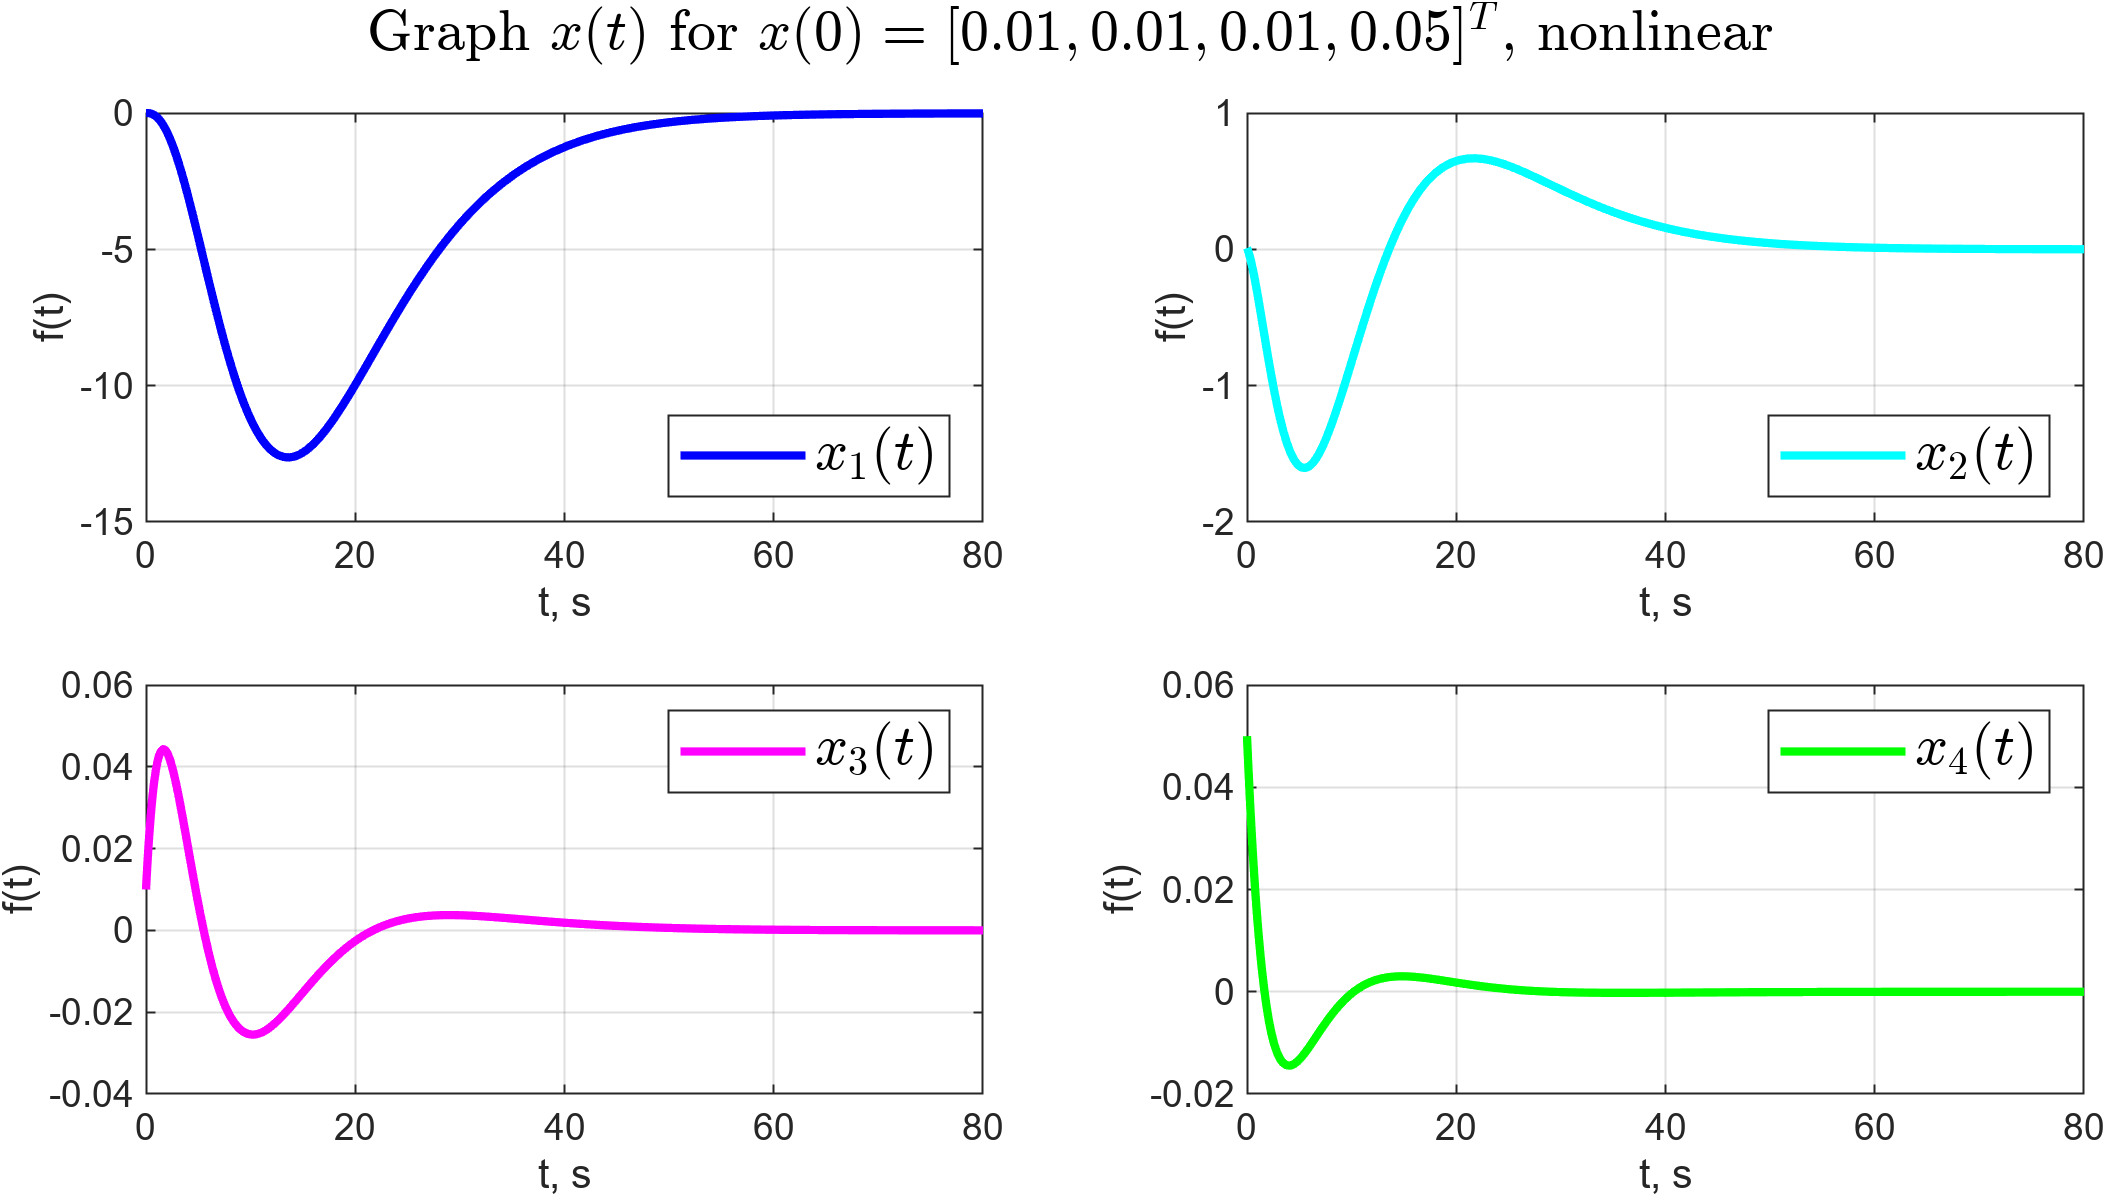
\includegraphics[width=1\linewidth]{pic/3_x_nlin_01_lg.png}}
\caption{График вектора состояния нелинейной системы, начальные условия $x_{01}$.}
\label{3_x_nlin_01_lg}
\end{figure}


\begin{figure}[!h]
\center{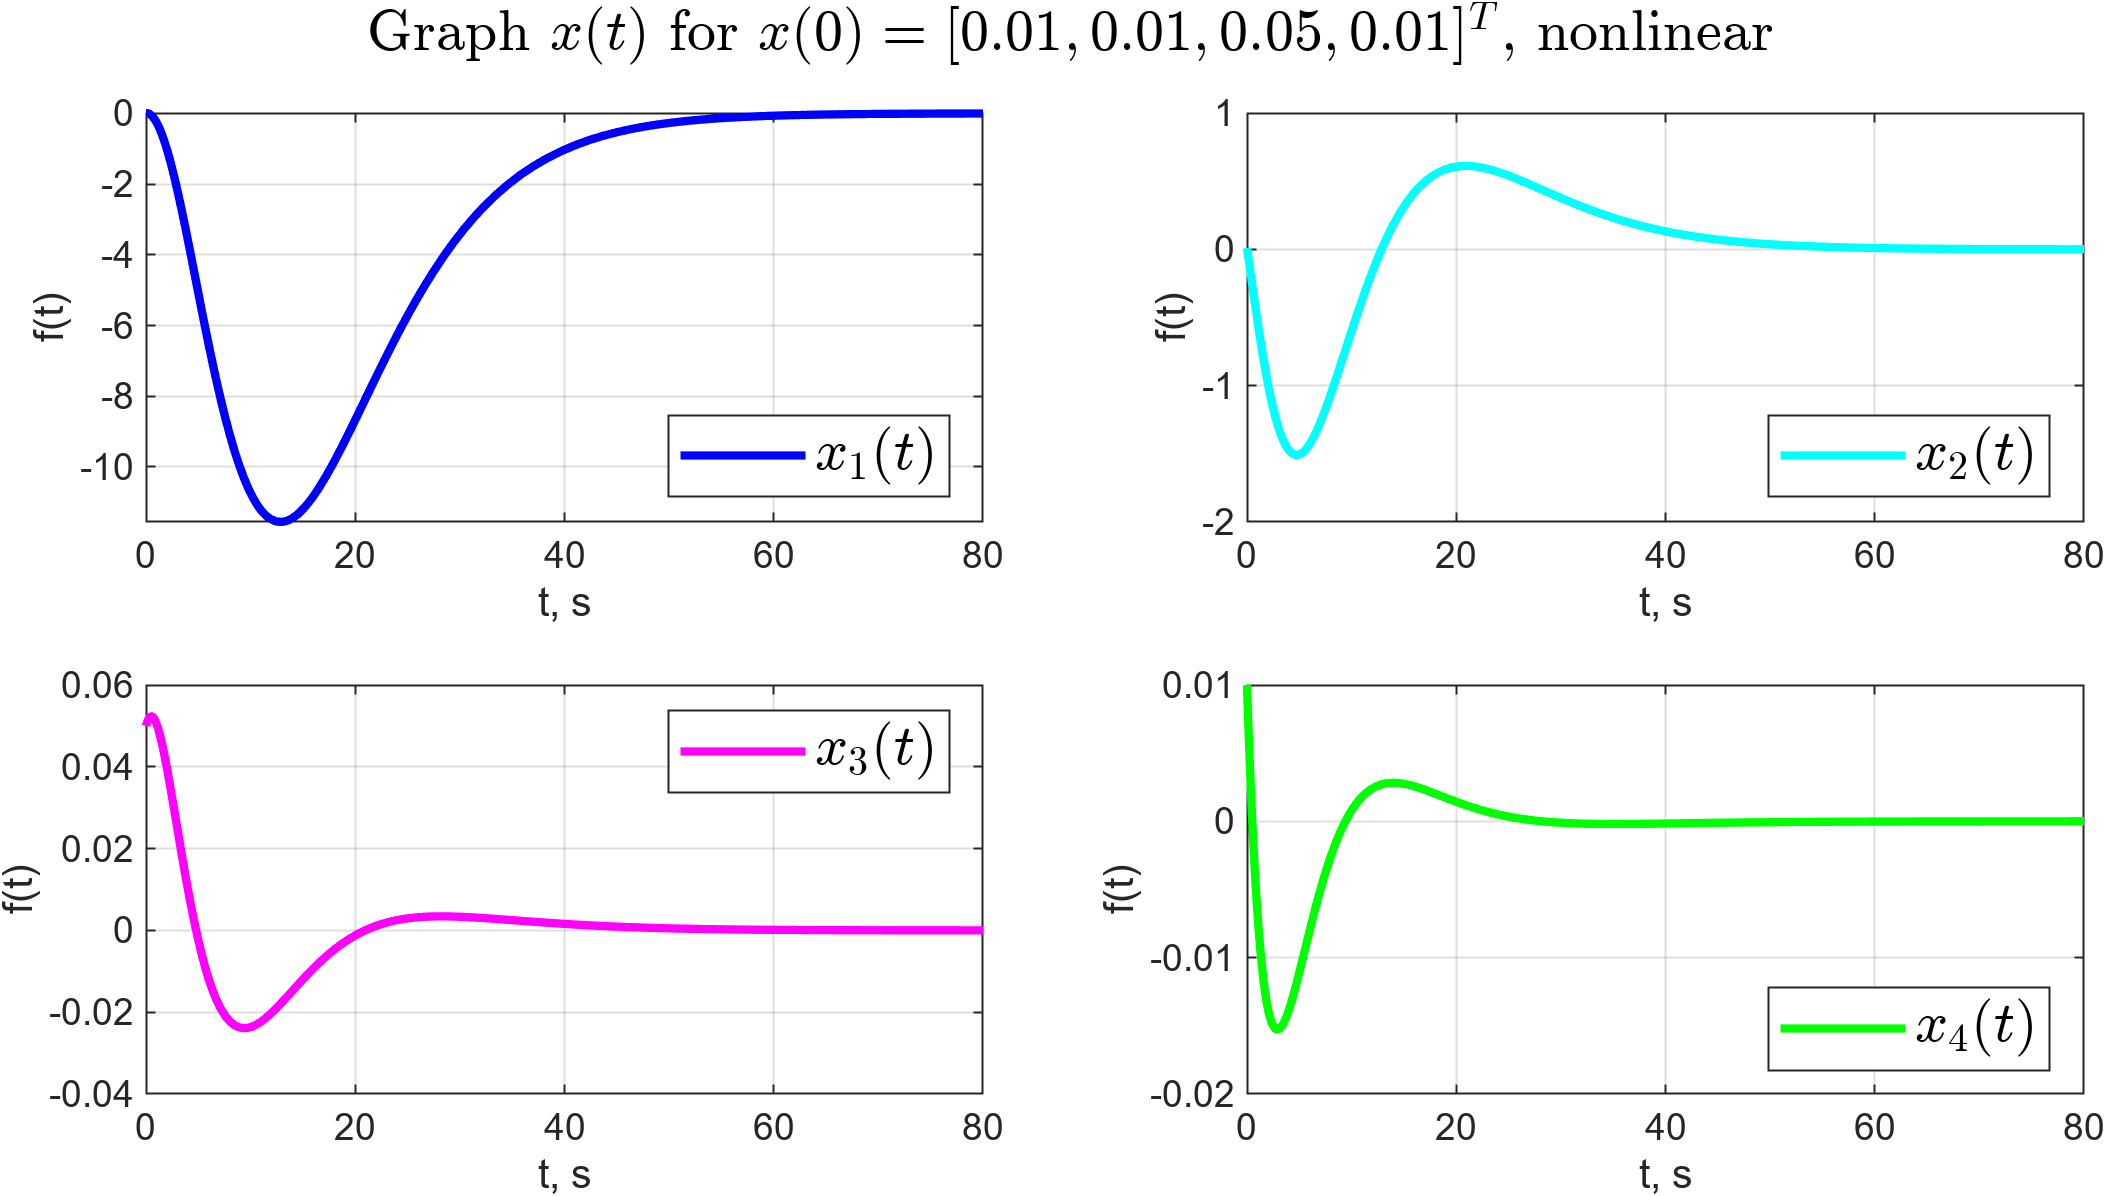
\includegraphics[width=1\linewidth]{pic/3_x_nlin_02_lg.png}}
\caption{График вектора состояния нелинейной системы, начальные условия $x_{02}$.}
\label{3_x_nlin_02_lg}
\end{figure}

\begin{figure}[!h]
\center{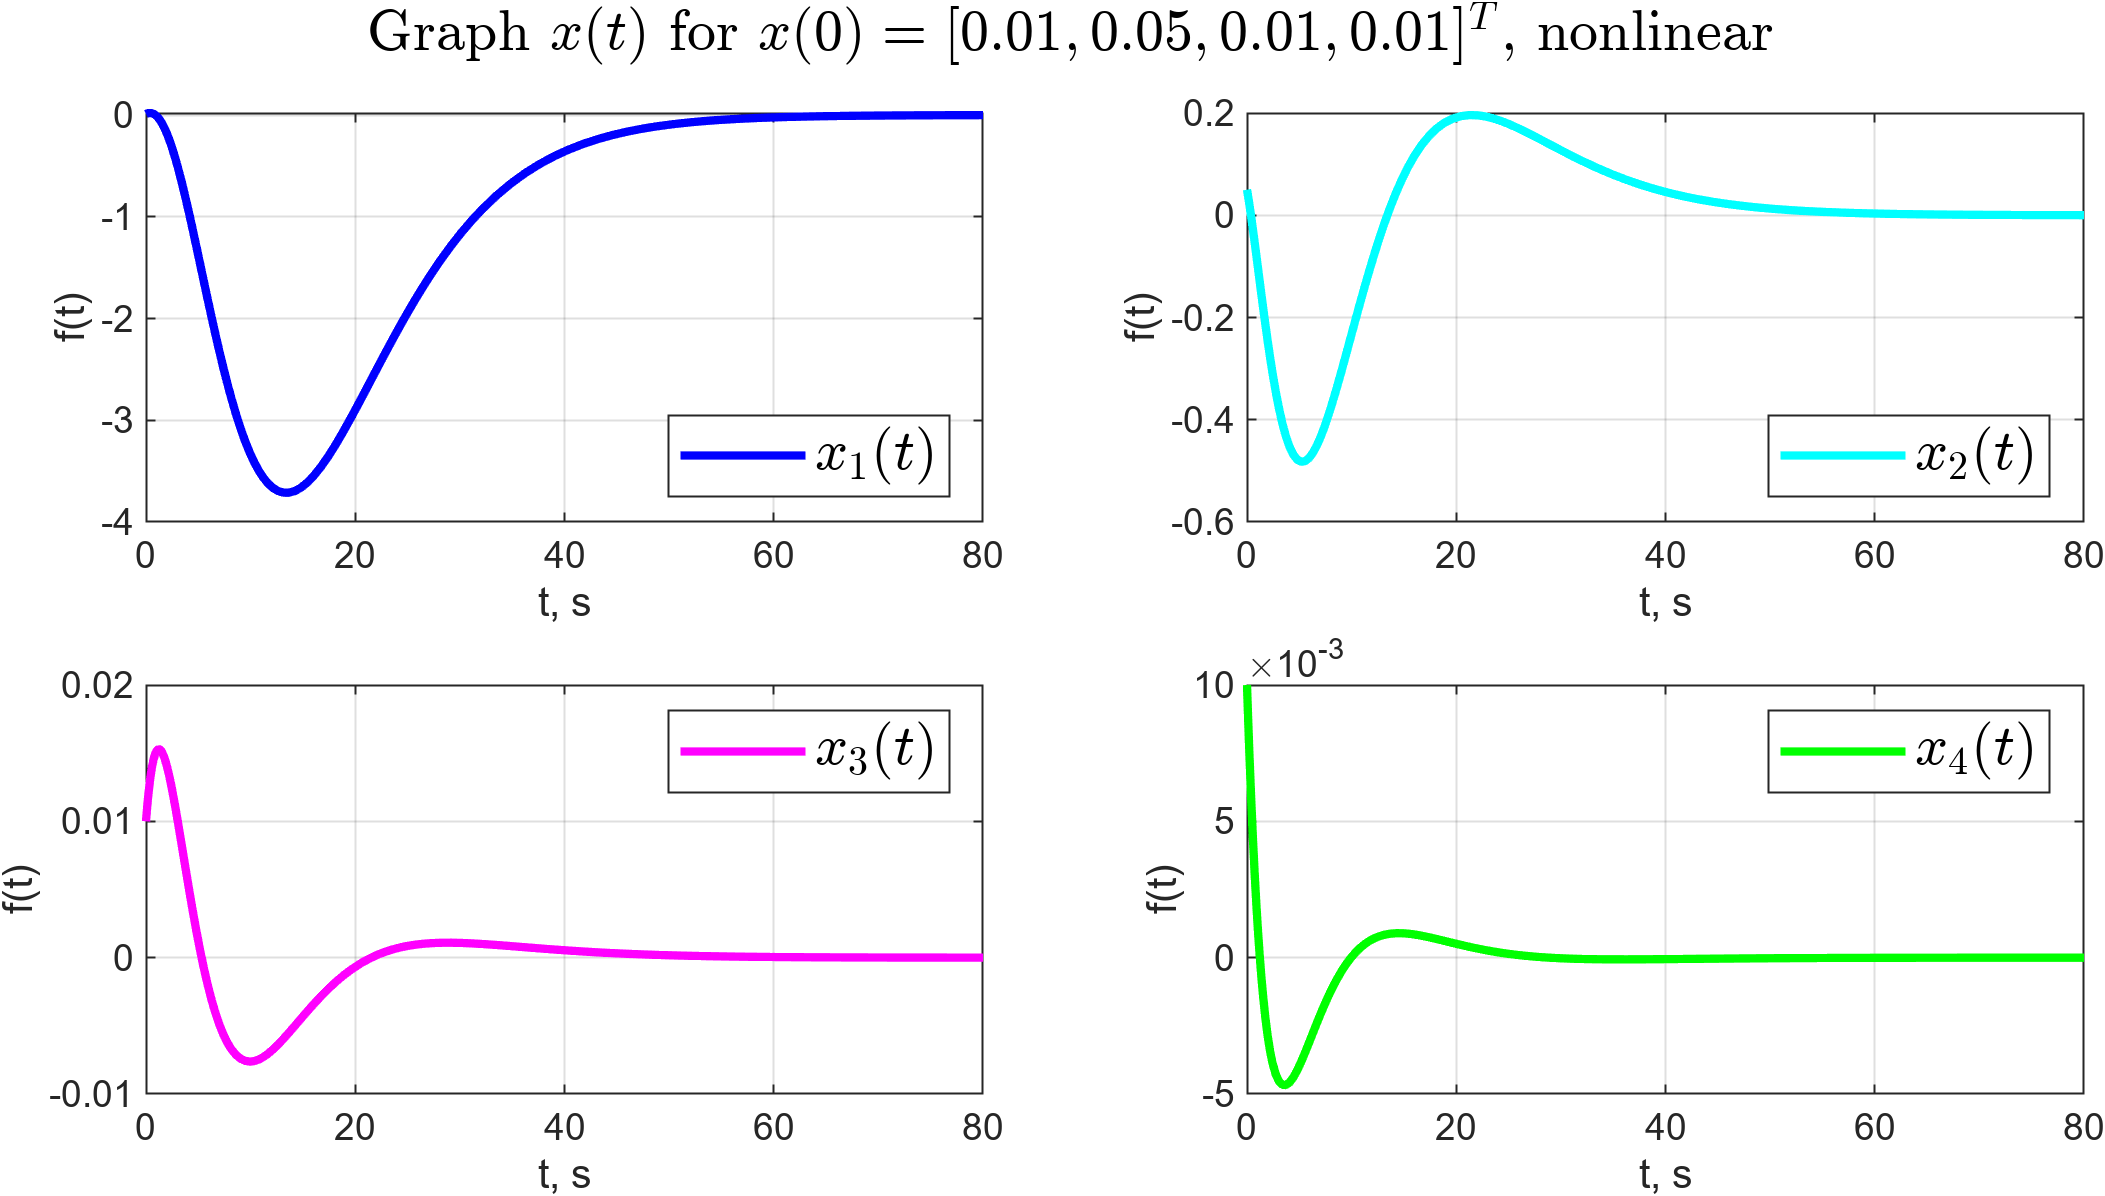
\includegraphics[width=1\linewidth]{pic/3_x_nlin_03_lg.png}}
\caption{График вектора состояния нелинейной системы, начальные условия $x_{03}$.}
\label{3_x_nlin_03_lg}
\end{figure}

\begin{figure}[!h]
\center{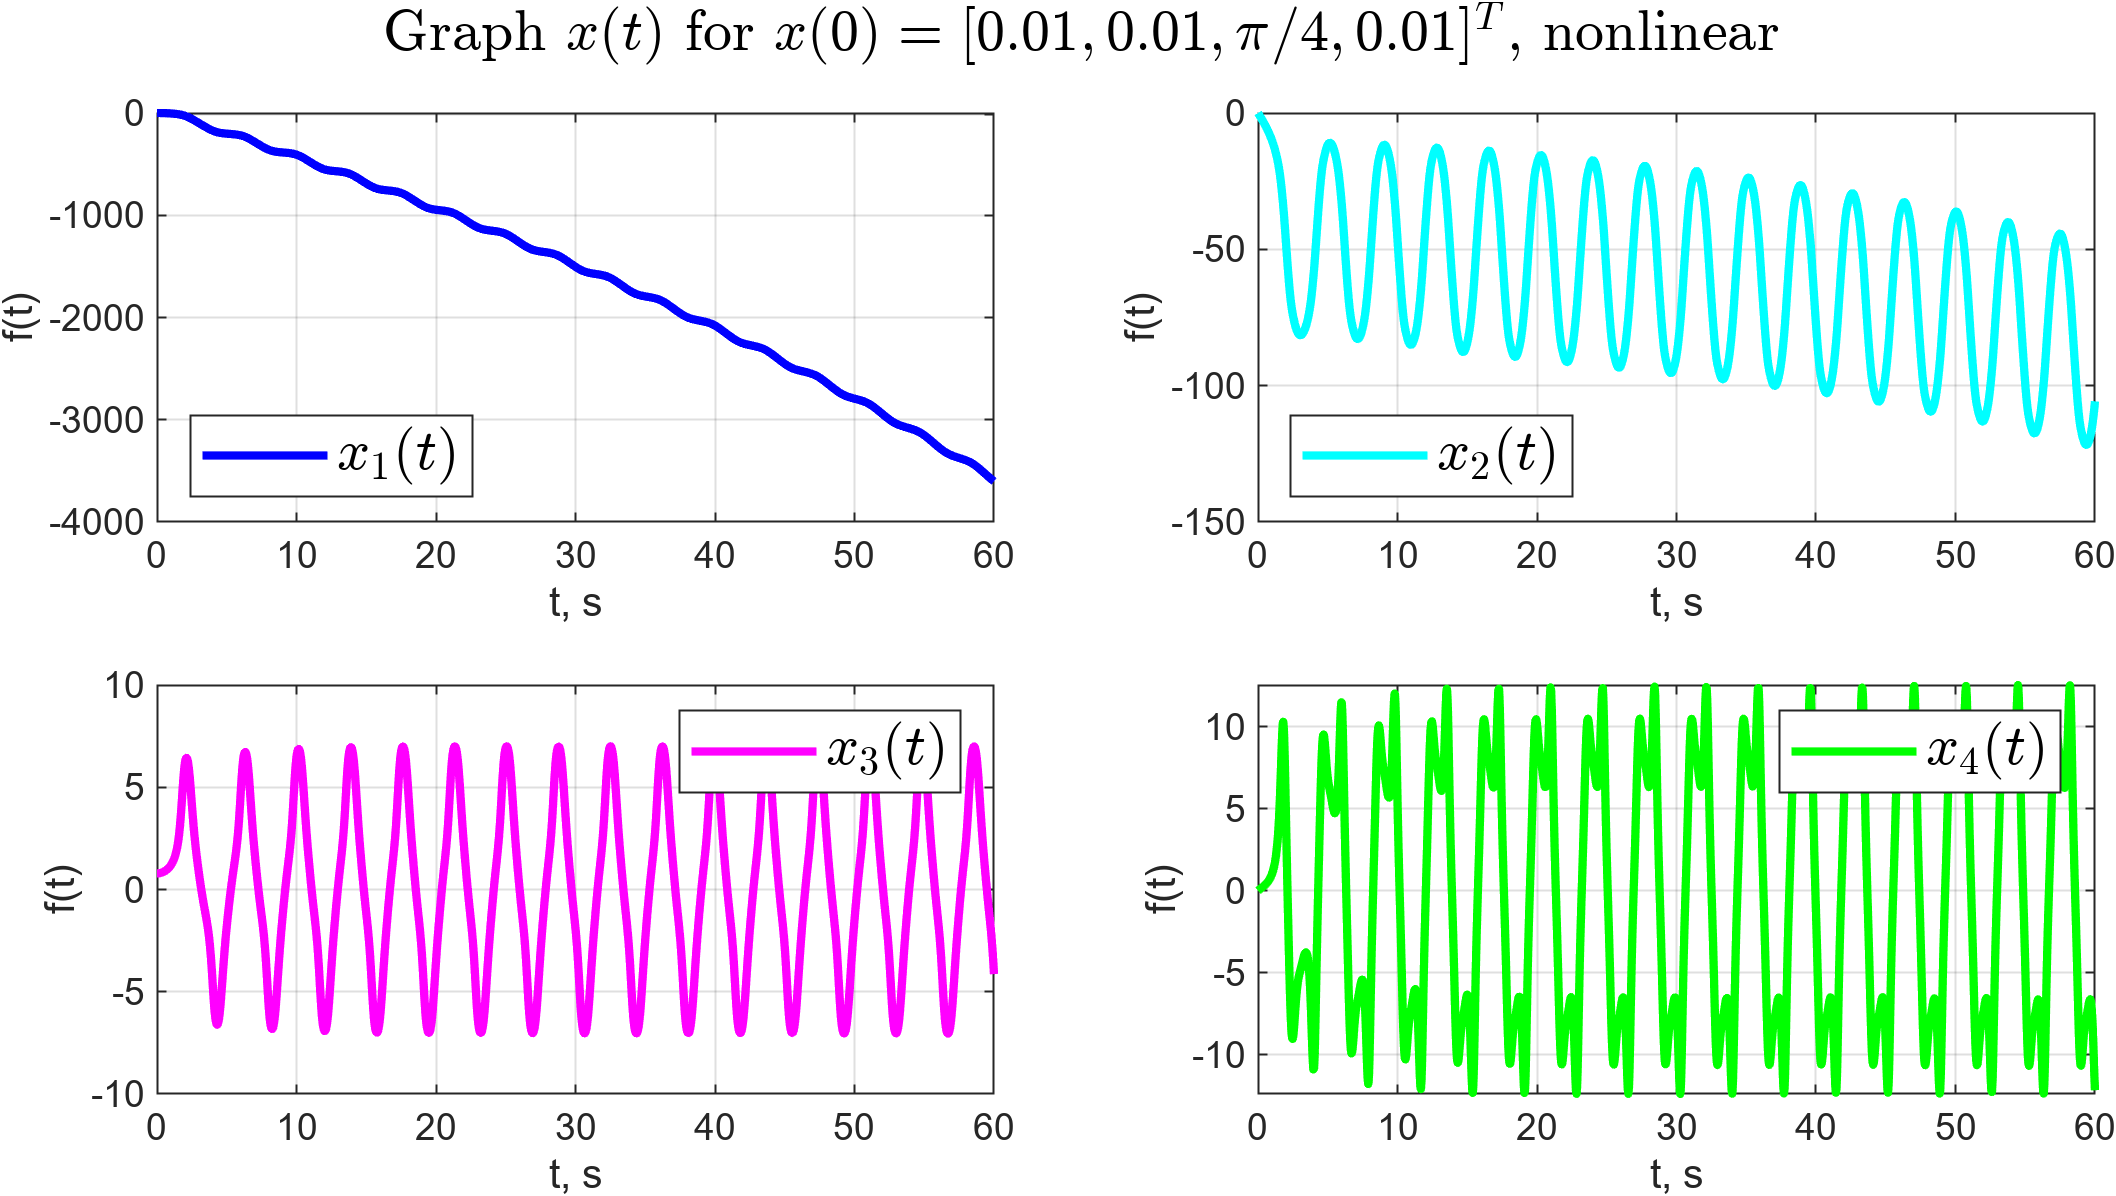
\includegraphics[width=1\linewidth]{pic/3_x_nlin_04_lg.png}}
\caption{График вектора состояния нелинейной системы, начальные условия $x_{04}$.}
\label{3_x_nlin_04_lg}
\end{figure}

\newpage
\,
\newpage
Заметим, что действительно при задании довольно большого угла начального отклонения маятника, система уже не стабилизируется синтезированным регулятором (рисунок \ref{3_x_nlin_04_lg}), также как и при большем начальном значении угловой скорости (рисунок \ref{3_x_nlin_05_lg}). 

\begin{figure}[!h]
\center{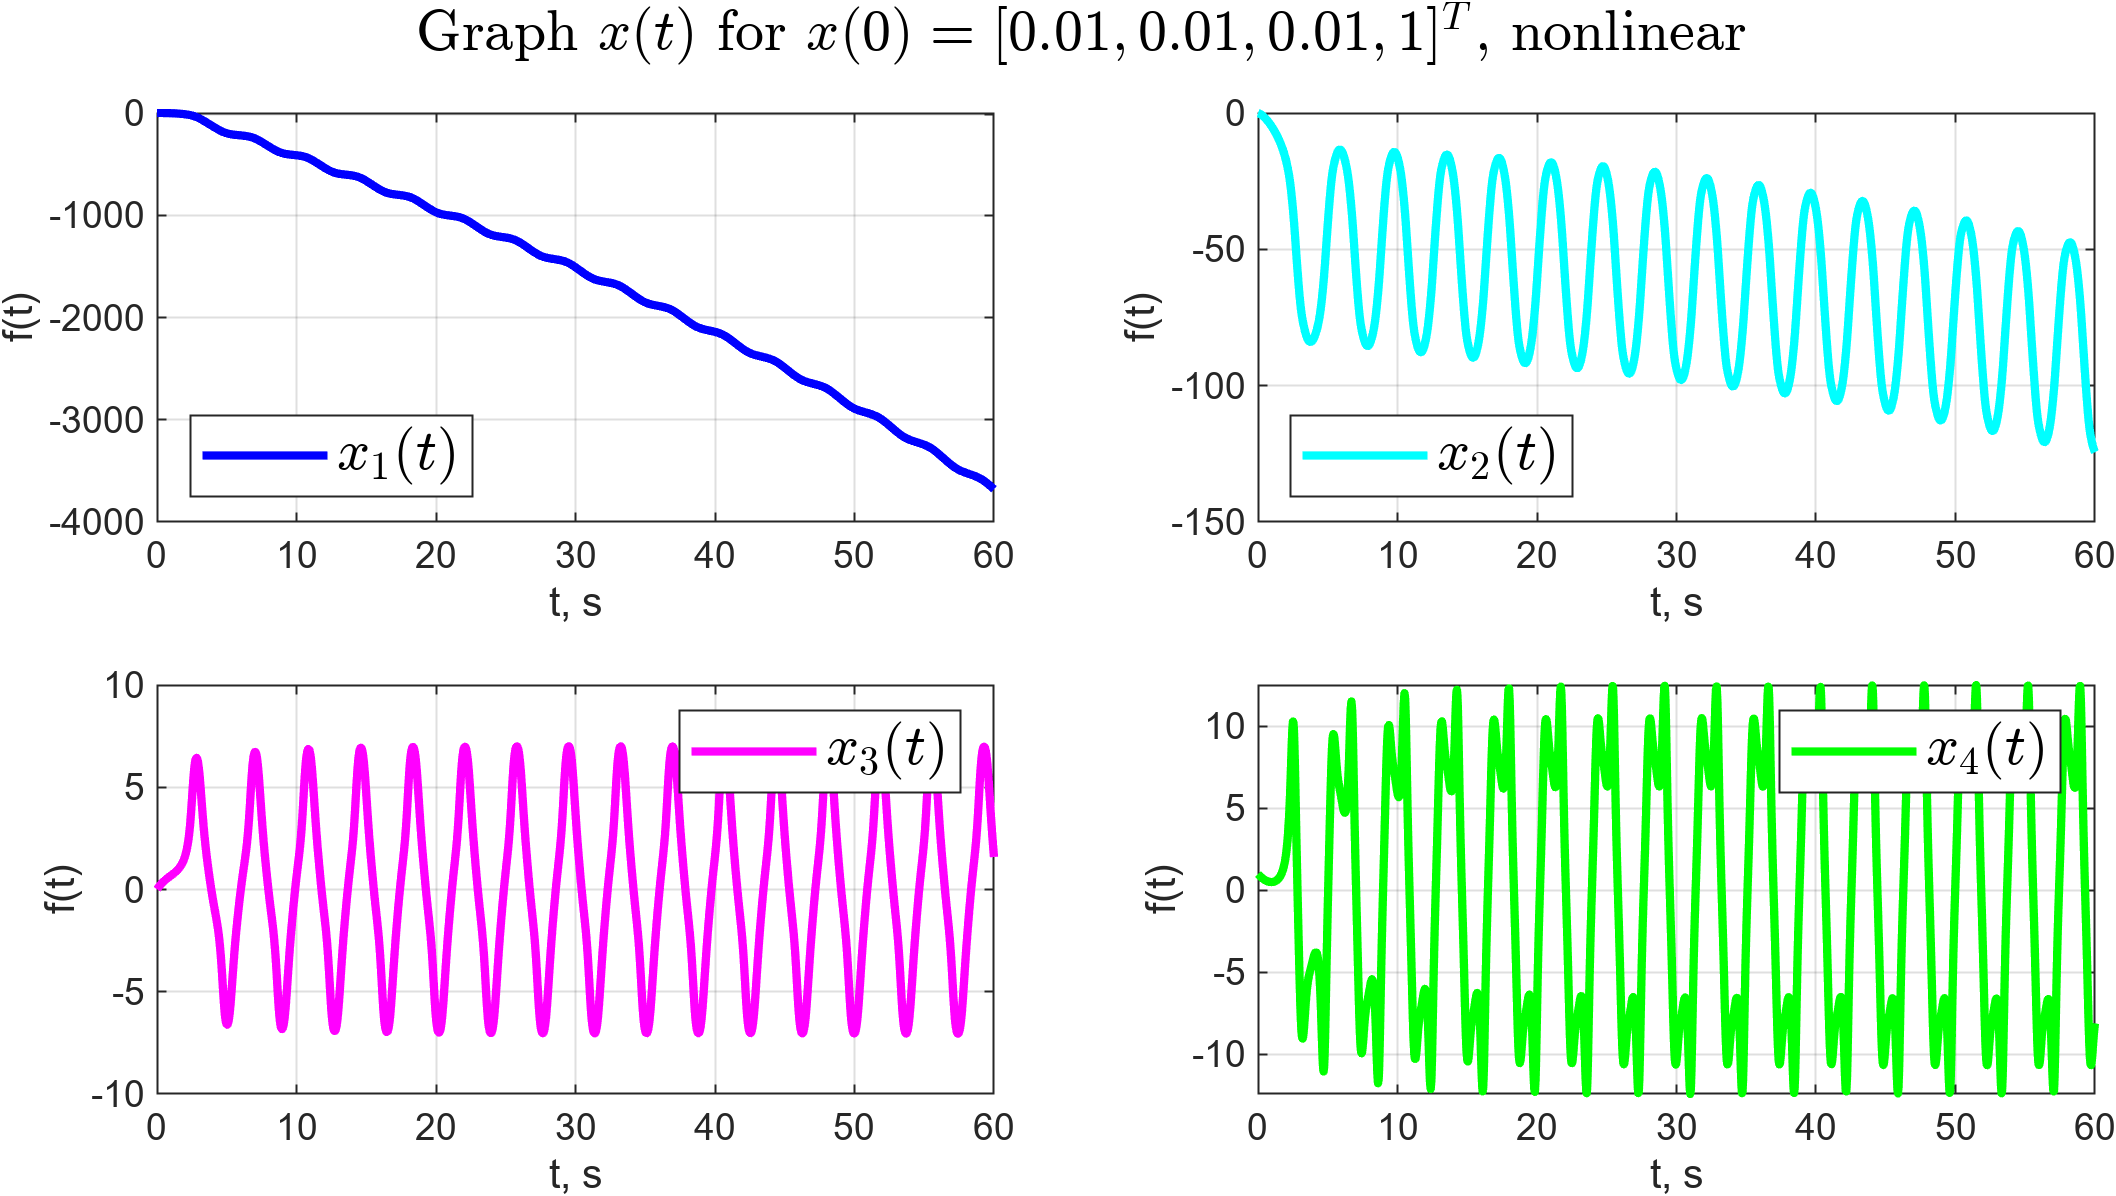
\includegraphics[width=1\linewidth]{pic/3_x_nlin_05_lg.png}}
\caption{График вектора состояния нелинейной системы, начальные условия $x_{05}$.}
\label{3_x_nlin_05_lg}
\end{figure}

Заметим также, что система нестабилизируется также при сильном увеличении начального значения скорости тележки (рисунок \ref{3_x_nlin_06_lg}) $$x_{06} = \begin{bmatrix}
    0.01 & 25 & 0.01 & 0.01
\end{bmatrix}^T$$ 

\begin{figure}[!h]
\center{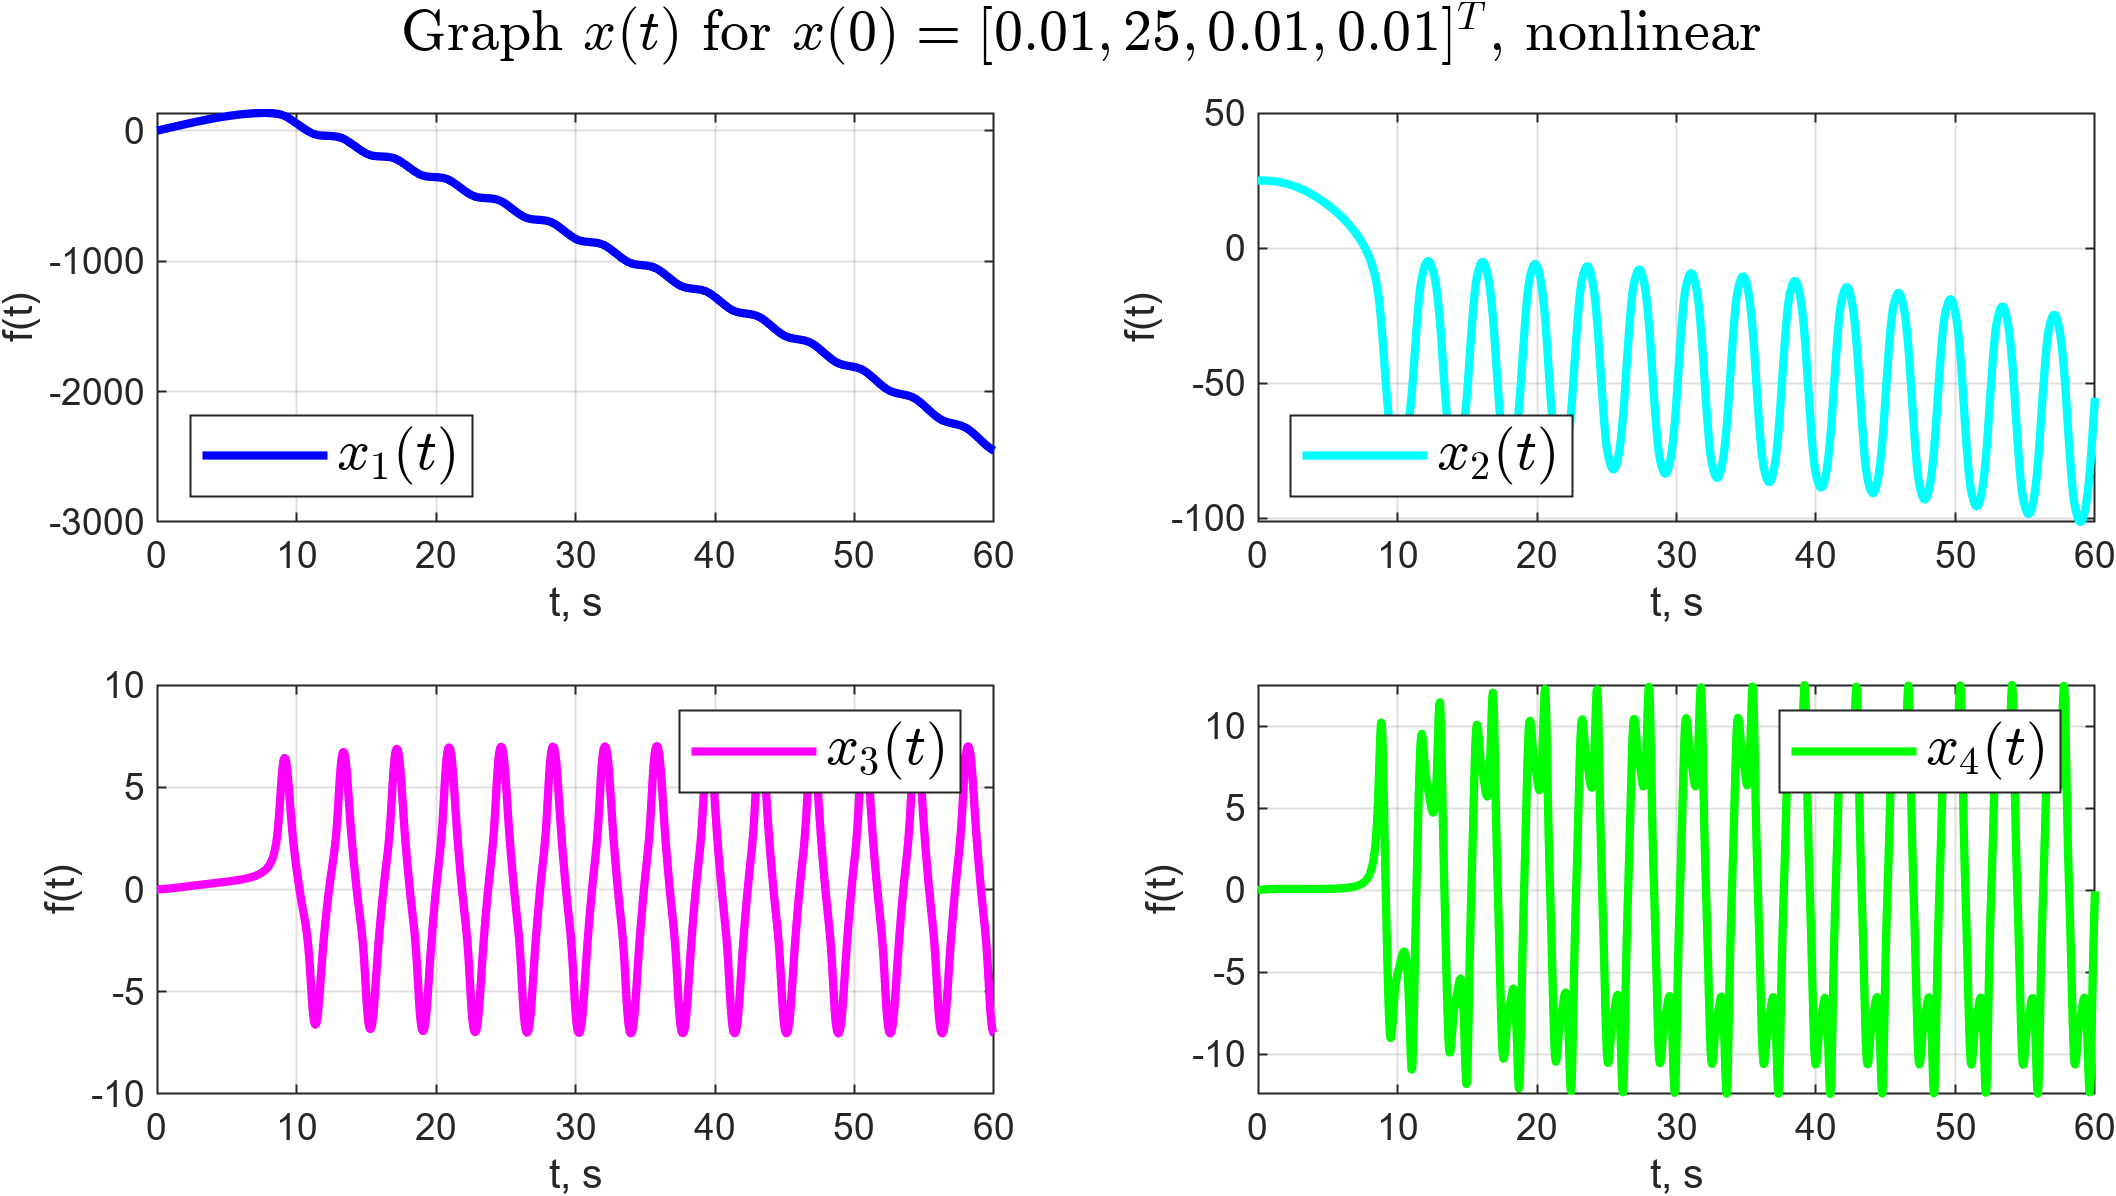
\includegraphics[width=1\linewidth]{pic/3_x_nlin_06_lg.png}}
\caption{График вектора состояния нелинейной системы, начальные условия $x_{06}$.}
\label{3_x_nlin_06_lg}
\end{figure}

Убедимся в том, что изменение начального значения координаты тележки до 100, не препятствует успешной стабилизации системы (рисунок \ref{3_x_nlin_07_lg})
$$x_{07} = \begin{bmatrix}
    100 & 0.01 & 0.01 & 0.01
\end{bmatrix}^T$$

\begin{figure}[!h]
\center{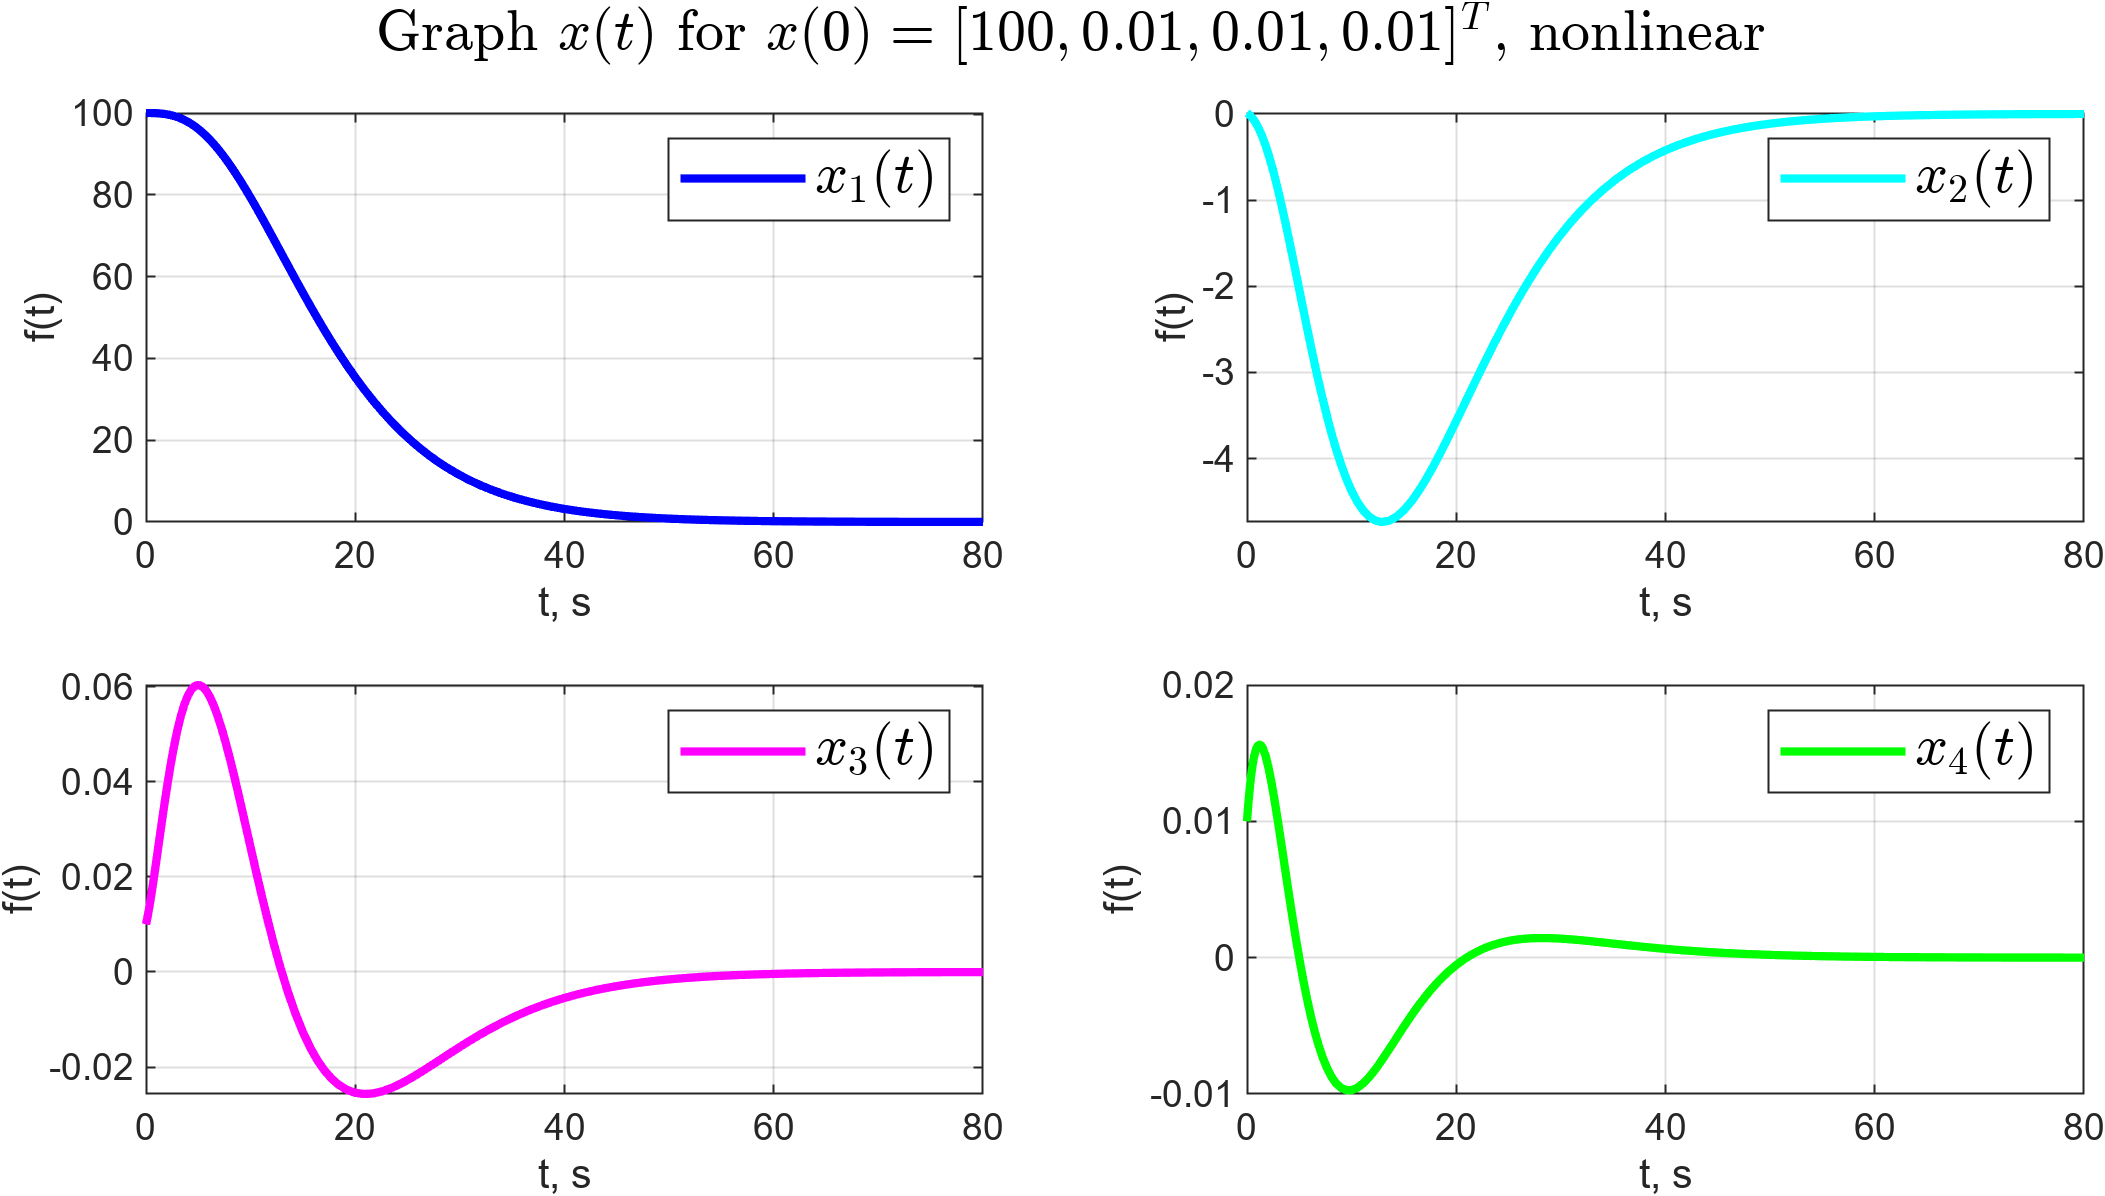
\includegraphics[width=1\linewidth]{pic/3_x_nlin_07_lg.png}}
\caption{График вектора состояния нелинейной системы, начальные условия $x_{07}$.}
\label{3_x_nlin_07_lg}
\end{figure}

Однако при повышении начального значения координаты тележки до 1000 стабилизировать систему с помощью синтезированного регулятора не удается (рисунок \ref{3_x_nlin_08_lg})
$$x_{08} = \begin{bmatrix}
    1000 & 0.01 & 0.01 & 0.01
\end{bmatrix}$$

\begin{figure}[!h]
\center{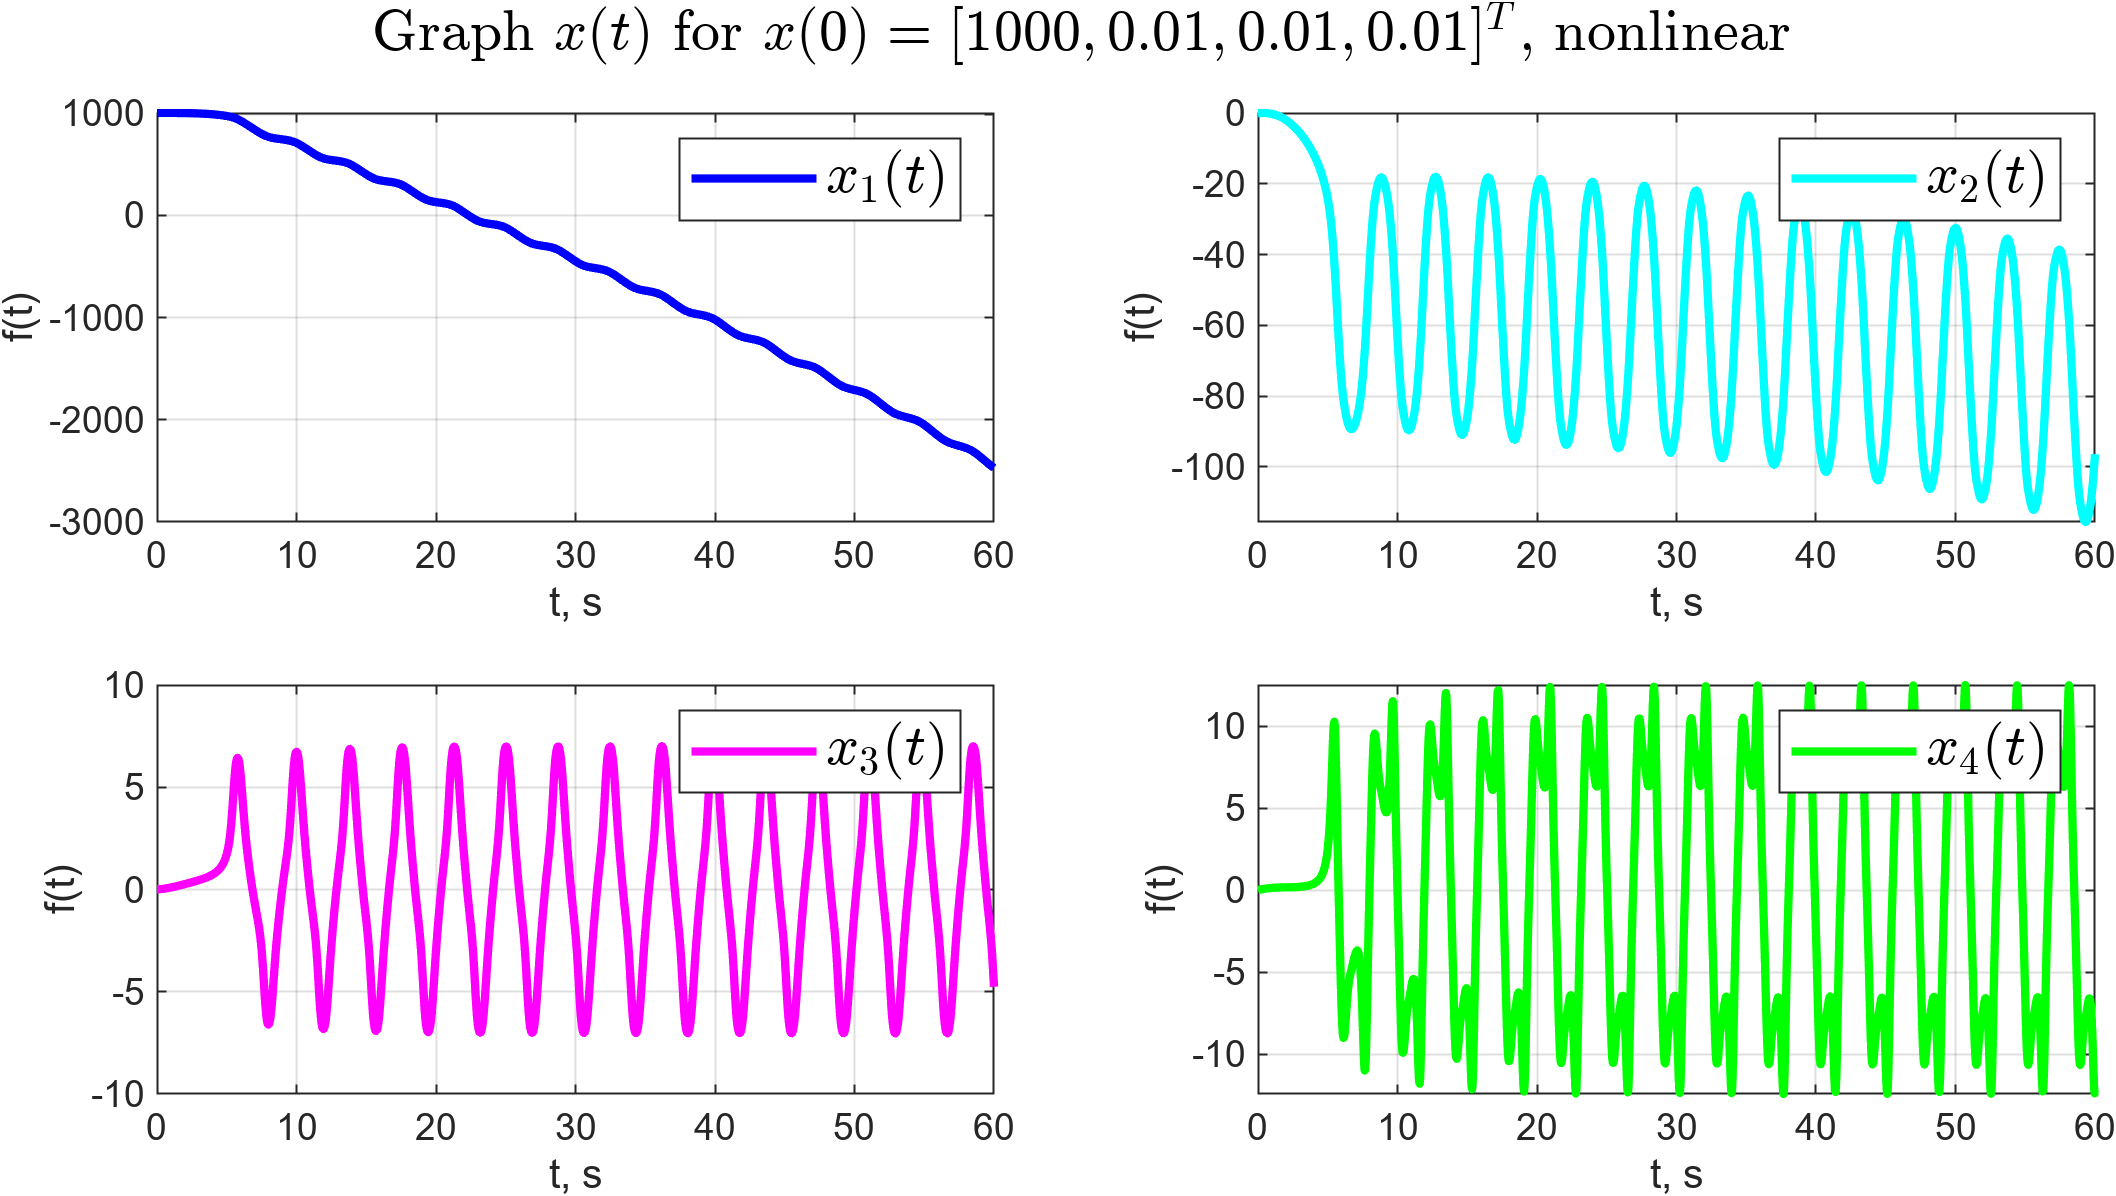
\includegraphics[width=1\linewidth]{pic/3_x_nlin_08_lg.png}}
\caption{График вектора состояния нелинейной системы, начальные условия $x_{08}$.}
\label{3_x_nlin_08_lg}
\end{figure}

\newpage
\subsection{Краткий вывод}
При начальных условиях, близких к нулю (наборы $x_{01}$, $x_{02}$, $x_{03}$), синтезированный регулятор позволяет стабилизировать систему. Начальные условия для угла отклонения и угловой скорости не позволяют стабилизировать систему, если принимают значения порядка единицы. В ходе дополнительного моделирования было выяснено, что критическим значением начальной скорости тележки, при котором регулятор не работает, является $\approx 18$ м/с. Критическим значением начальной координаты тележки, при котором перестает работать регулятор, является $\approx 400$ м. 


\section{Исследование регулятора по состоянию}

Исследуем влияние выбранных собственных чисел на максимальное отклонение маятника от вертикали, максимальное горизонтальное смещение тележки и максимальное значение управляющего сигнала при управлении нелинейной системой (\ref{1_model_full}).

Будем рассматривать следующие спектры замкнутой системы

\begin{equation*}
  \begin{matrix}
      \sigma_1 = \{ -0.3, -0.25, -0.2, -0.15 \}, & \sigma_2 = \{ -3, -2.5, -2, -1.5 \},\\
      \sigma_3 = \{ -1, -2, -3 \pm 3i \}, & \sigma_4 = \{ -10, -20, -30 \pm 10i \}
 \end{matrix}
\end{equation*}

в качестве начальных условий примем вектор $$x(0) = \begin{bmatrix}
    0.01&&
    0.01&&
    0.01&&
    0.01
\end{bmatrix}^T$$

\begin{table}[h]
\centering
\caption{Значения управления \( u(t) \) и состояний системы}
\label{tab:results}
\begin{tabular}{ccccc}
\toprule
Спектр & $\max |\varphi|$ & $\max |a|$ & $\max |u|$ \\
\midrule
$\sigma_1$  &  0.0152  &  3.9533  &  43.4049  \\
$\sigma_2$  &  0.0101  &  0.0389  &  227.1943  \\
$\sigma_3$  &  0.0101  &  0.0329  &  277.5976  \\
$\sigma_4$  &  0.0499  &  0.0935  &  96295  \\
\bottomrule
\end{tabular}
\end{table}

\begin{figure}[!h]
\center{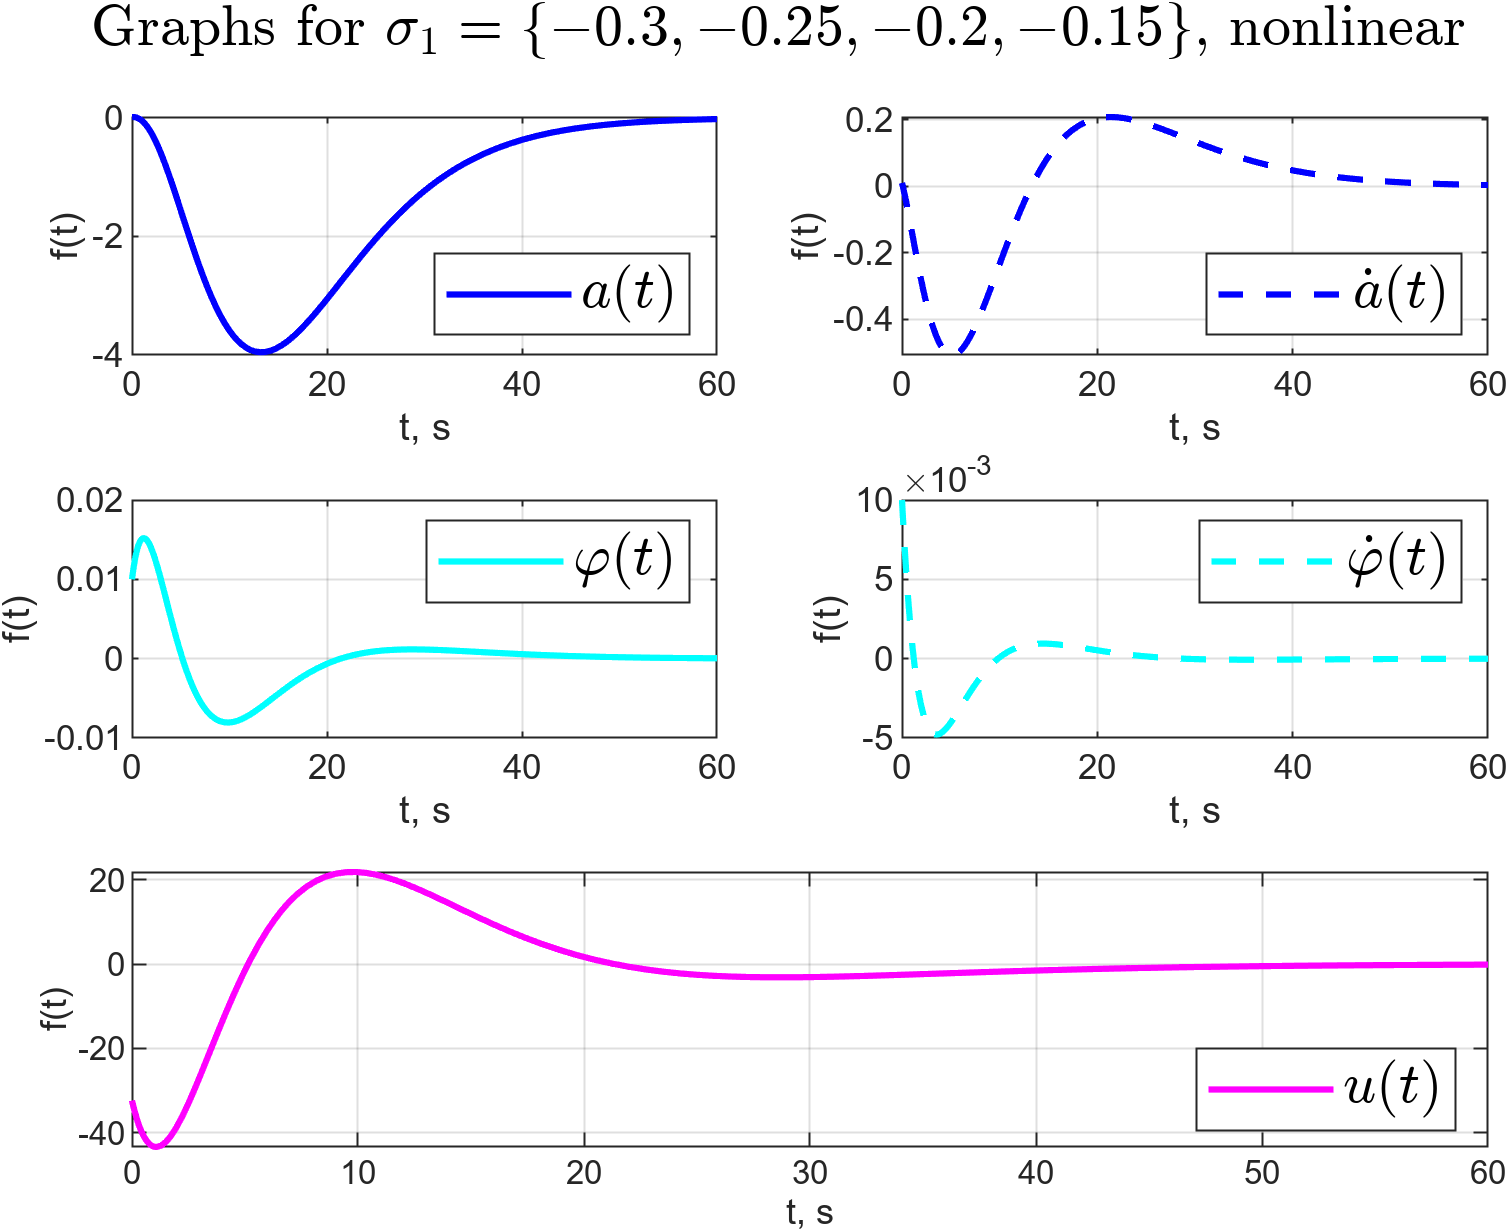
\includegraphics[width=1\linewidth]{pic/3_x_nlin_s1.png}}
\caption{Графики компонент вектора состояния системы и $u(t)$ для $\sigma_1$.}
\label{3_x_nlin_s1}
\end{figure}

\begin{figure}[!h]
\center{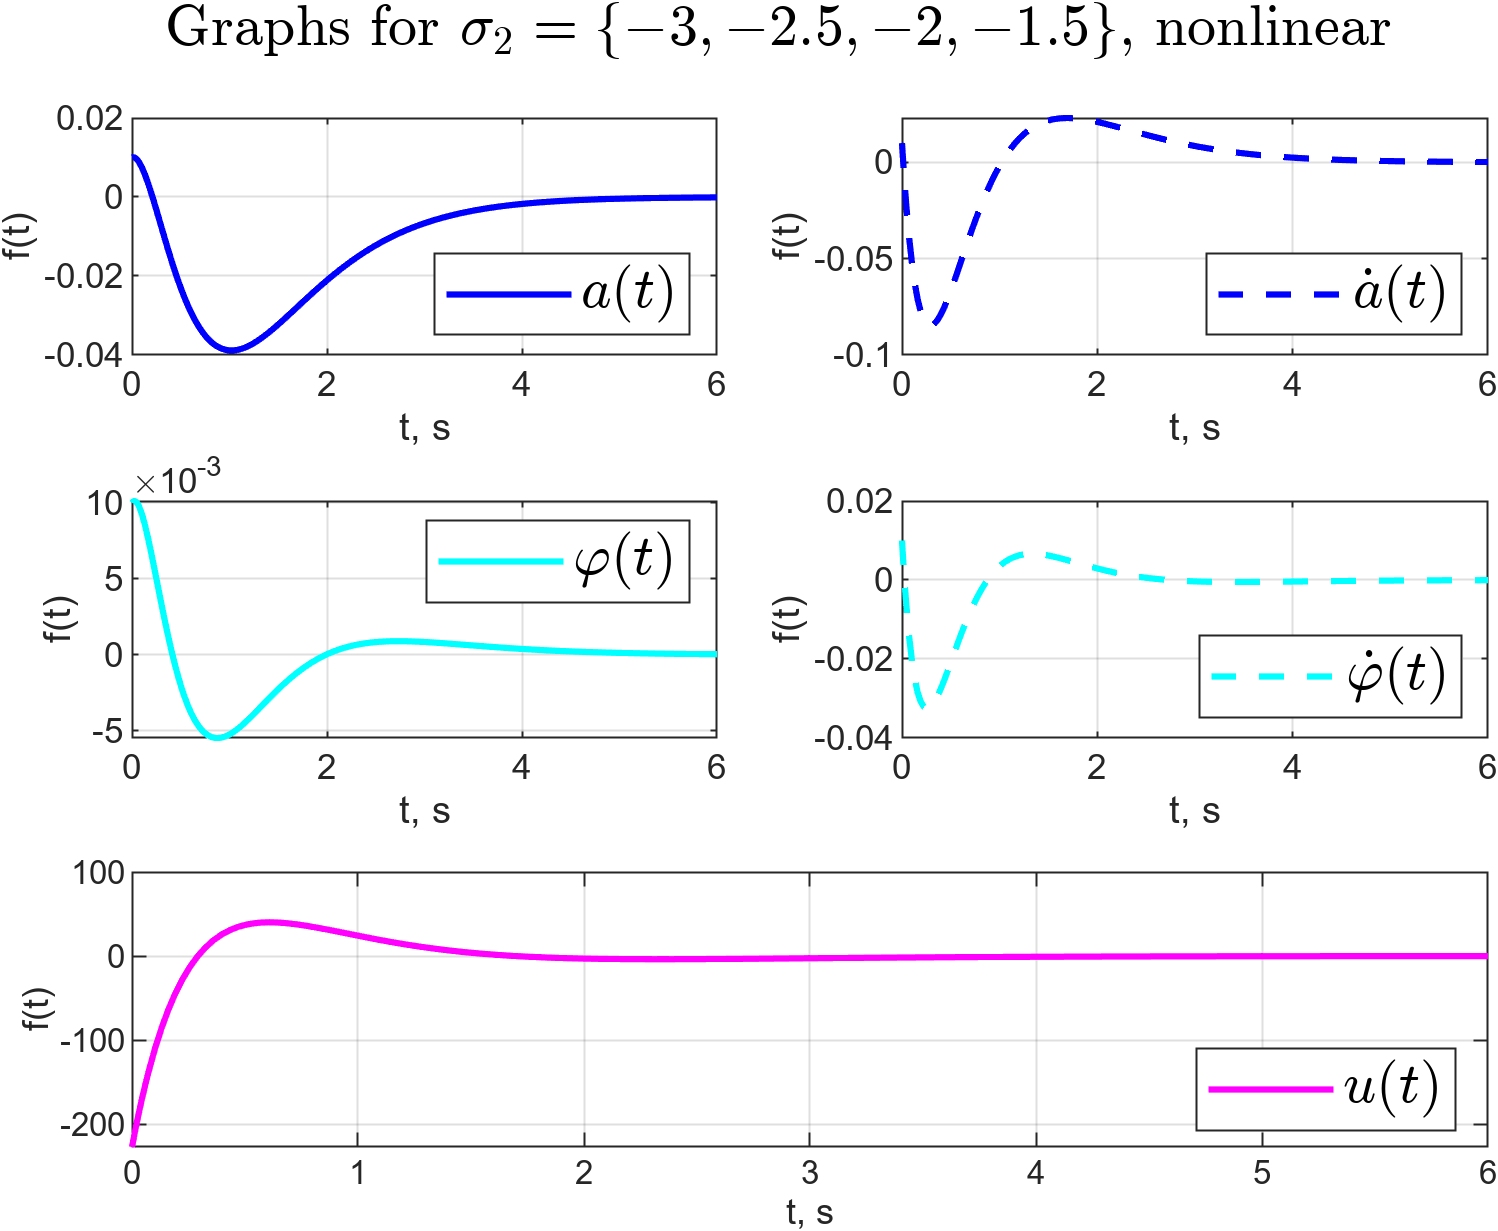
\includegraphics[width=1\linewidth]{pic/3_x_nlin_s2.png}}
\caption{Графики компонент вектора состояния системы и $u(t)$ для $\sigma_2$.}
\label{3_x_nlin_s2}
\end{figure}

\begin{figure}[!h]
\center{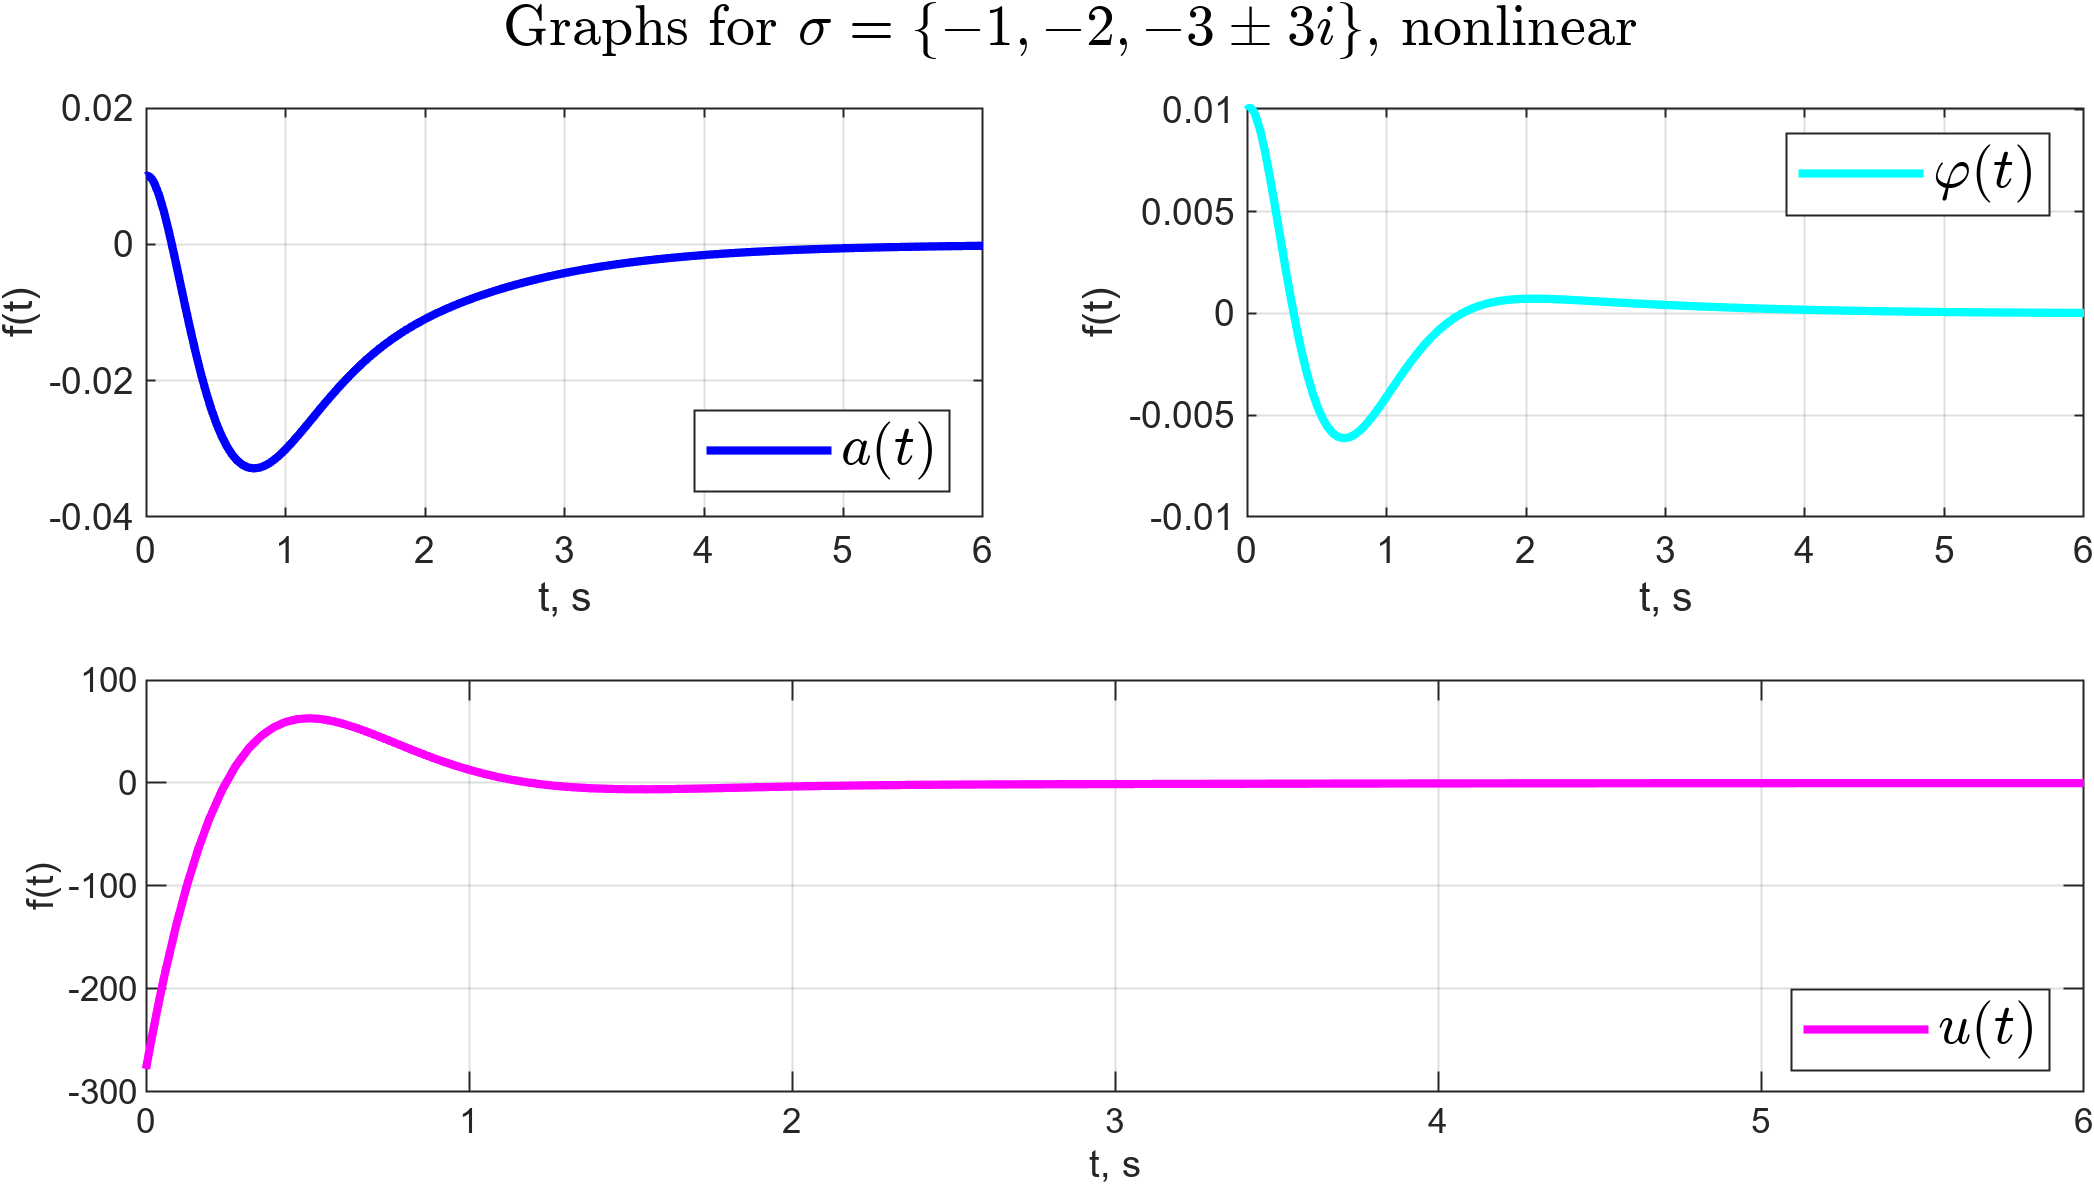
\includegraphics[width=1\linewidth]{pic/3_x_nlin_s3.png}}
\caption{Графики компонент вектора состояния системы и $u(t)$ для $\sigma_3$.}
\label{3_x_nlin_s3}
\end{figure}

\begin{figure}[!h]
\center{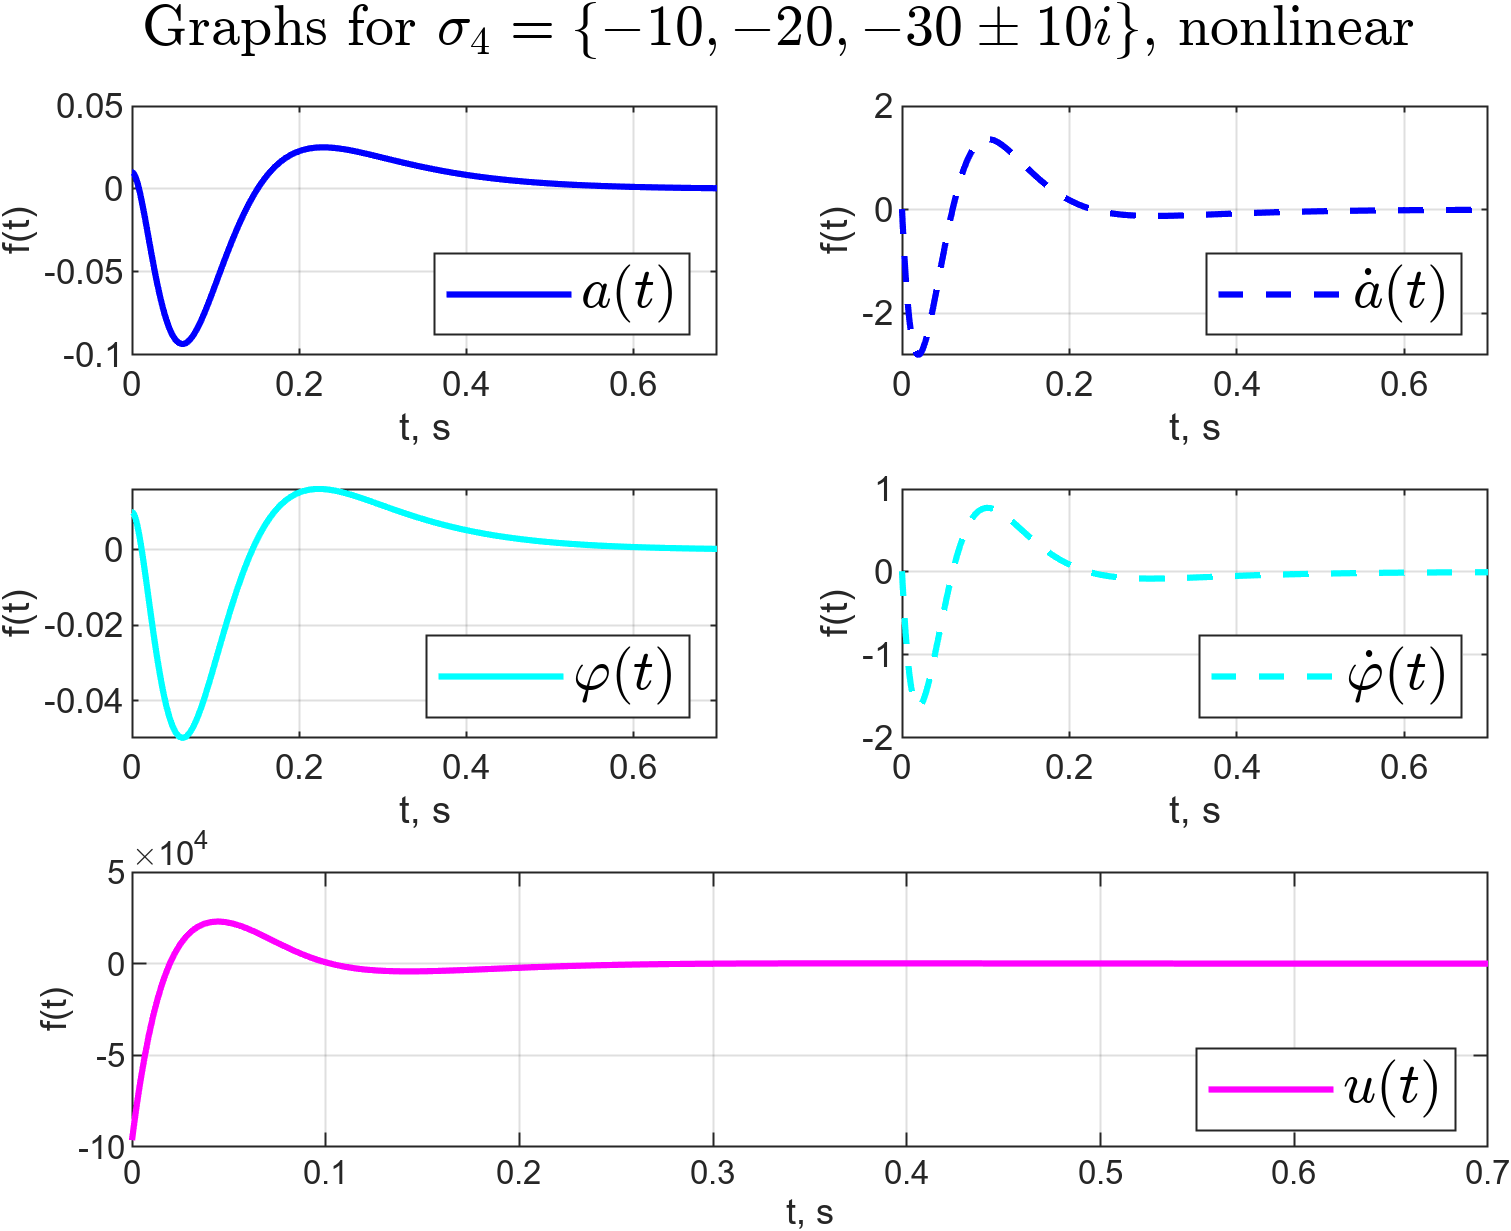
\includegraphics[width=1\linewidth]{pic/3_x_nlin_s4.png}}
\caption{Графики компонент вектора состояния системы и $u(t)$ для $\sigma_4$.}
\label{3_x_nlin_s4}
\end{figure}

Заметим, что при увеличении модулей значений спектра, возрастает максимальное значение управляющего сигнала, но уменьшается время, через которое вектор состояния системы становится неотличим от нуля. Результаты моделирования представлены на рисунках \ref{3_x_nlin_s1}-\ref{3_x_nlin_s4} (в данном задании для большей наглядности компоненты вектра состояния на графиках обозначены соответствующими физическими величинами).

\section{Синтез наблюдателя}

\subsection{Наблюдатель полной размерности}
Запишем наблюдатель полной размерности

\begin{equation}
    \begin{cases}
        \hat{y} = C \hat{x},\\
        \dot{\hat{x}} = A \hat{x} + Bu + L( \hat{y} - y)
    \end{cases}
\end{equation}


Для нахождения матрицы регулятора $L$ будем решать систему, содержающую уравнение Сильвестра

\begin{equation}
    \label{3_sil_obs}
    \begin{cases}
        \Gamma Q - Q A = YC\\
        L = Q^{-1}Y
    \end{cases}
\end{equation}
Запишем условия существования решения $Q$: $\sigma(A) \cap \sigma(\Gamma) = \emptyset$, $(\Gamma,Y)$ -- управляема, $(C, A)$ -- наблюдаема. Заметим, что последнее условие выполнено. 

Зададимся спектром $\sigma = \{ -1, -2, -3, -4  \}$, запишем подходящие матрицы $\Gamma$ и $Y$

\begin{equation}
\Gamma=
    \begin{bmatrix}
    -1	&0	&0	&0\\
0	&-2	&0	&0\\
0	&0&	-3	&0\\
0	&0	&0	&-4
\end{bmatrix}, \, \, 
Y  = \begin{bmatrix}
    1 & 1\\
    1 & 1\\
    1 & 1\\
    1 & 1
\end{bmatrix}
\end{equation}

Убедимся, что условие $(\Gamma,Y)$ -- управляема выполнено, составим матрицу управляемости и найдем ее ранг

\begin{multline}
    U = \begin{bmatrix}
    Y & \Gamma Y & \Gamma^2 Y &\Gamma^3 Y &
    \end{bmatrix} = \begin{bmatrix}
        1	&1&	-1&	-1&	1	&1&	-1&	-1\\
1	&1	&-2	&-2&	4&	4	&-8&	-8\\
1	&1	&-3&	-3&	9	&9	&-27&	-27\\
1	&1	&-4&	-4&	16&	16&	-64&	-64
    \end{bmatrix} \Rightarrow\\
    \Rightarrow rank(U) = 4
\end{multline}

Ранг матрицы $U$ равен размерности системы, $(\Gamma,Y)$ -- управляема.

Решим систему (\ref{3_sil_obs}) и получим $L$

\begin{equation}
    L = \begin{bmatrix}
        7.7918	&7.7918\\
2.2438	&2.2438\\
-17.7918	&-17.7918\\
-43.0833	&-43.0833
    \end{bmatrix}
\end{equation}

Выберем систему, замкнутую систему со спектром $\sigma_2 = \{ -3, -2.5, -2, -1.5 \}$ из исследованных ранее в пункте 3.2.


Запишем начальные условия системы и наблюдателя

\begin{equation}
    \begin{matrix}
        x(0) = \begin{bmatrix}
    0.01&&
    0.01&&
    0.01&&
    0.01
\end{bmatrix}^T\\
 \hat{x}(0) = \begin{bmatrix}
    0&&
    0&&
    0&&
    0
\end{bmatrix}^T
    \end{matrix}
\end{equation}

Построим графики $x(t)$ и $\hat{x}$ (рисунок \ref{3_xx_nlin_02_L1}) и график ошибки $e(t) = \hat{x}(t) - x(t)$ (рисунок \ref{3_e_nlin_02_L1}). Заметим, что синтезированный наблюдатель работает довольно успешно: ошибка наблюдения становится визуально неотличима от нуля после $t=2$ с.

\begin{figure}[!h]
\center{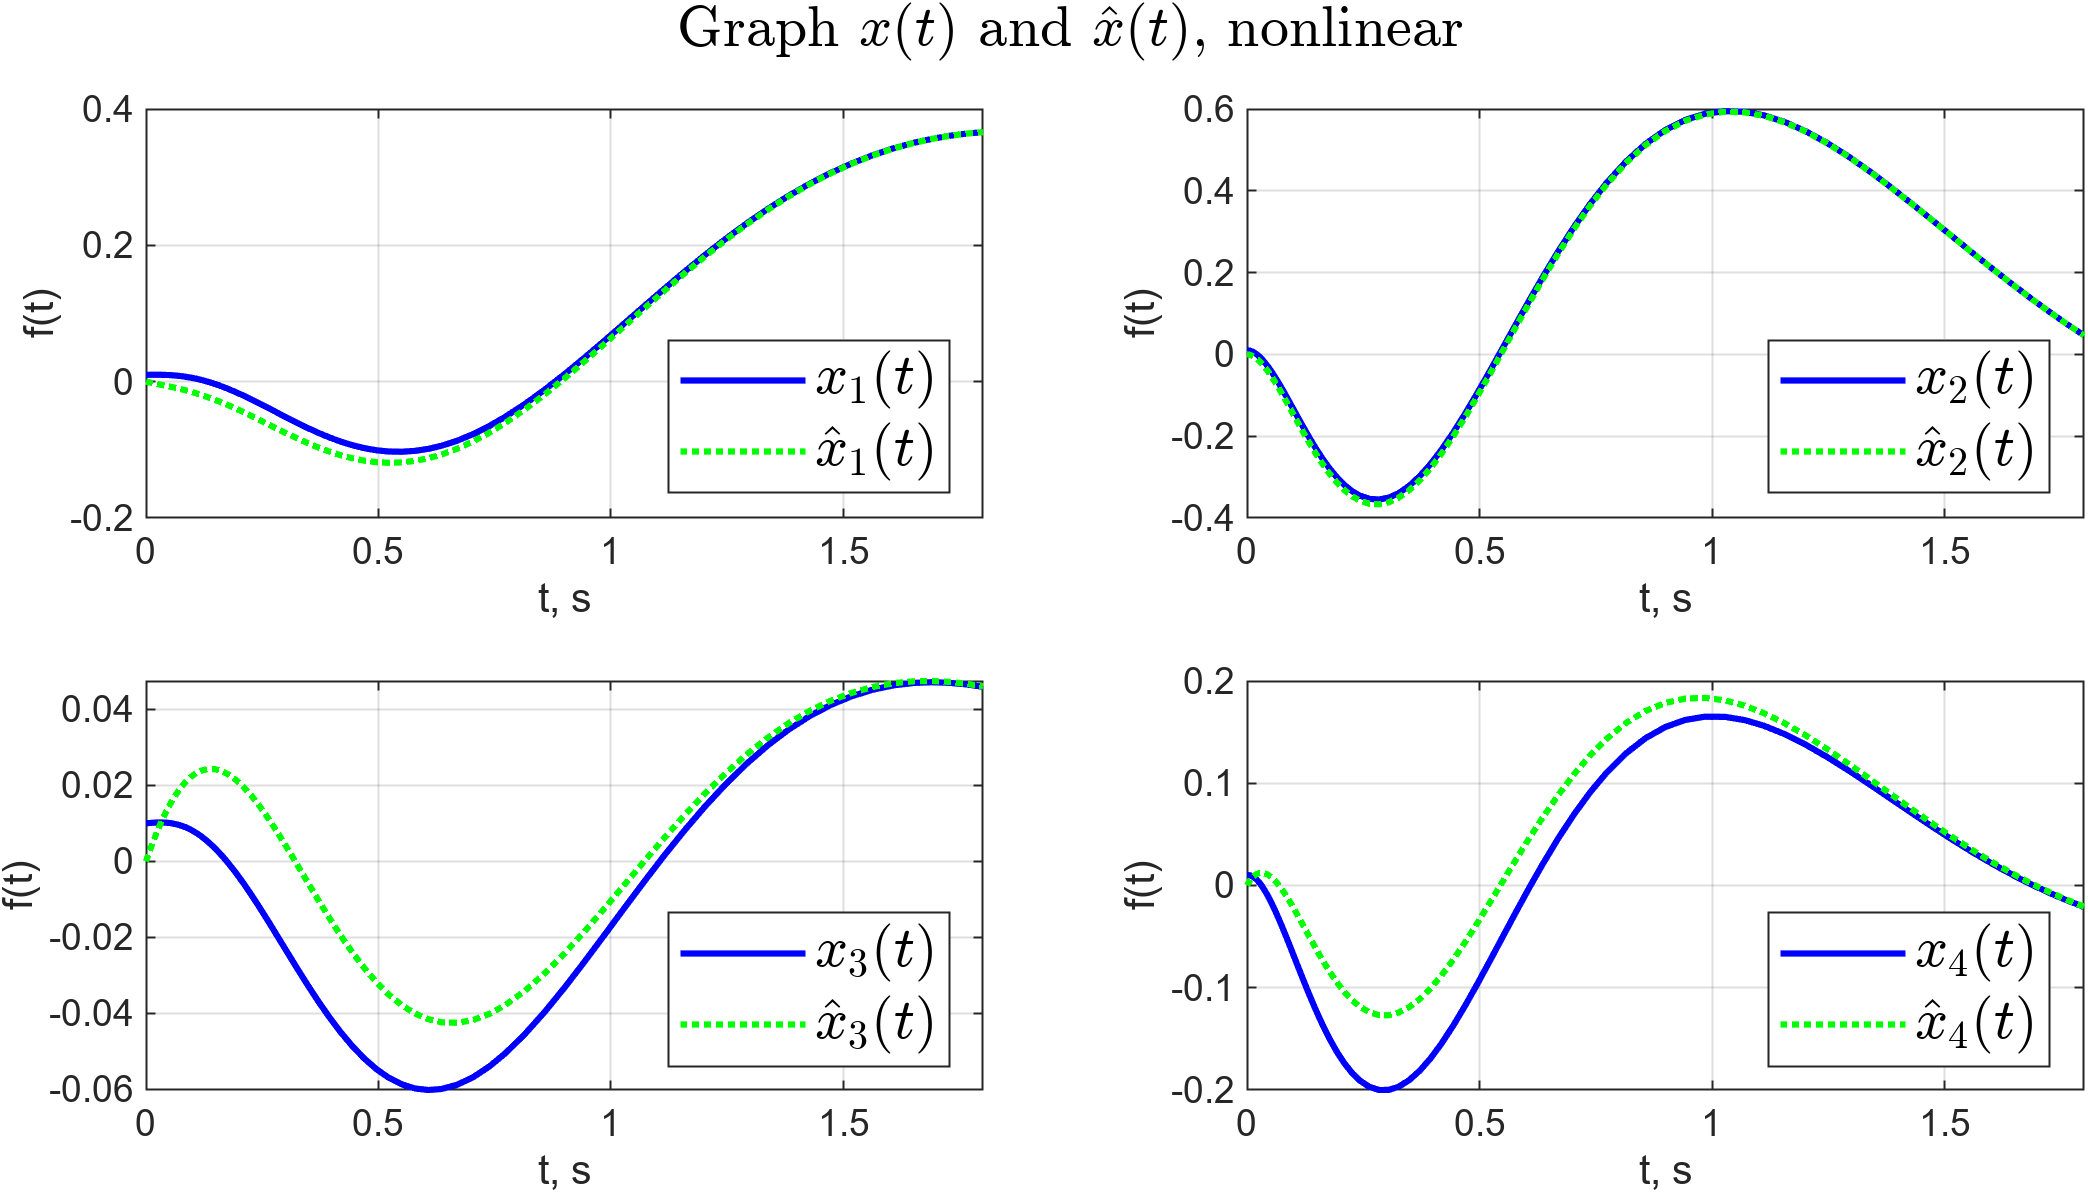
\includegraphics[width=1\linewidth]{pic/3_xx_nlin_02_L1.png}}
\caption{Графики $x(t)$ и $\hat{x}(t)$.}
\label{3_xx_nlin_02_L1}
\end{figure}


\begin{figure}[!h]
\center{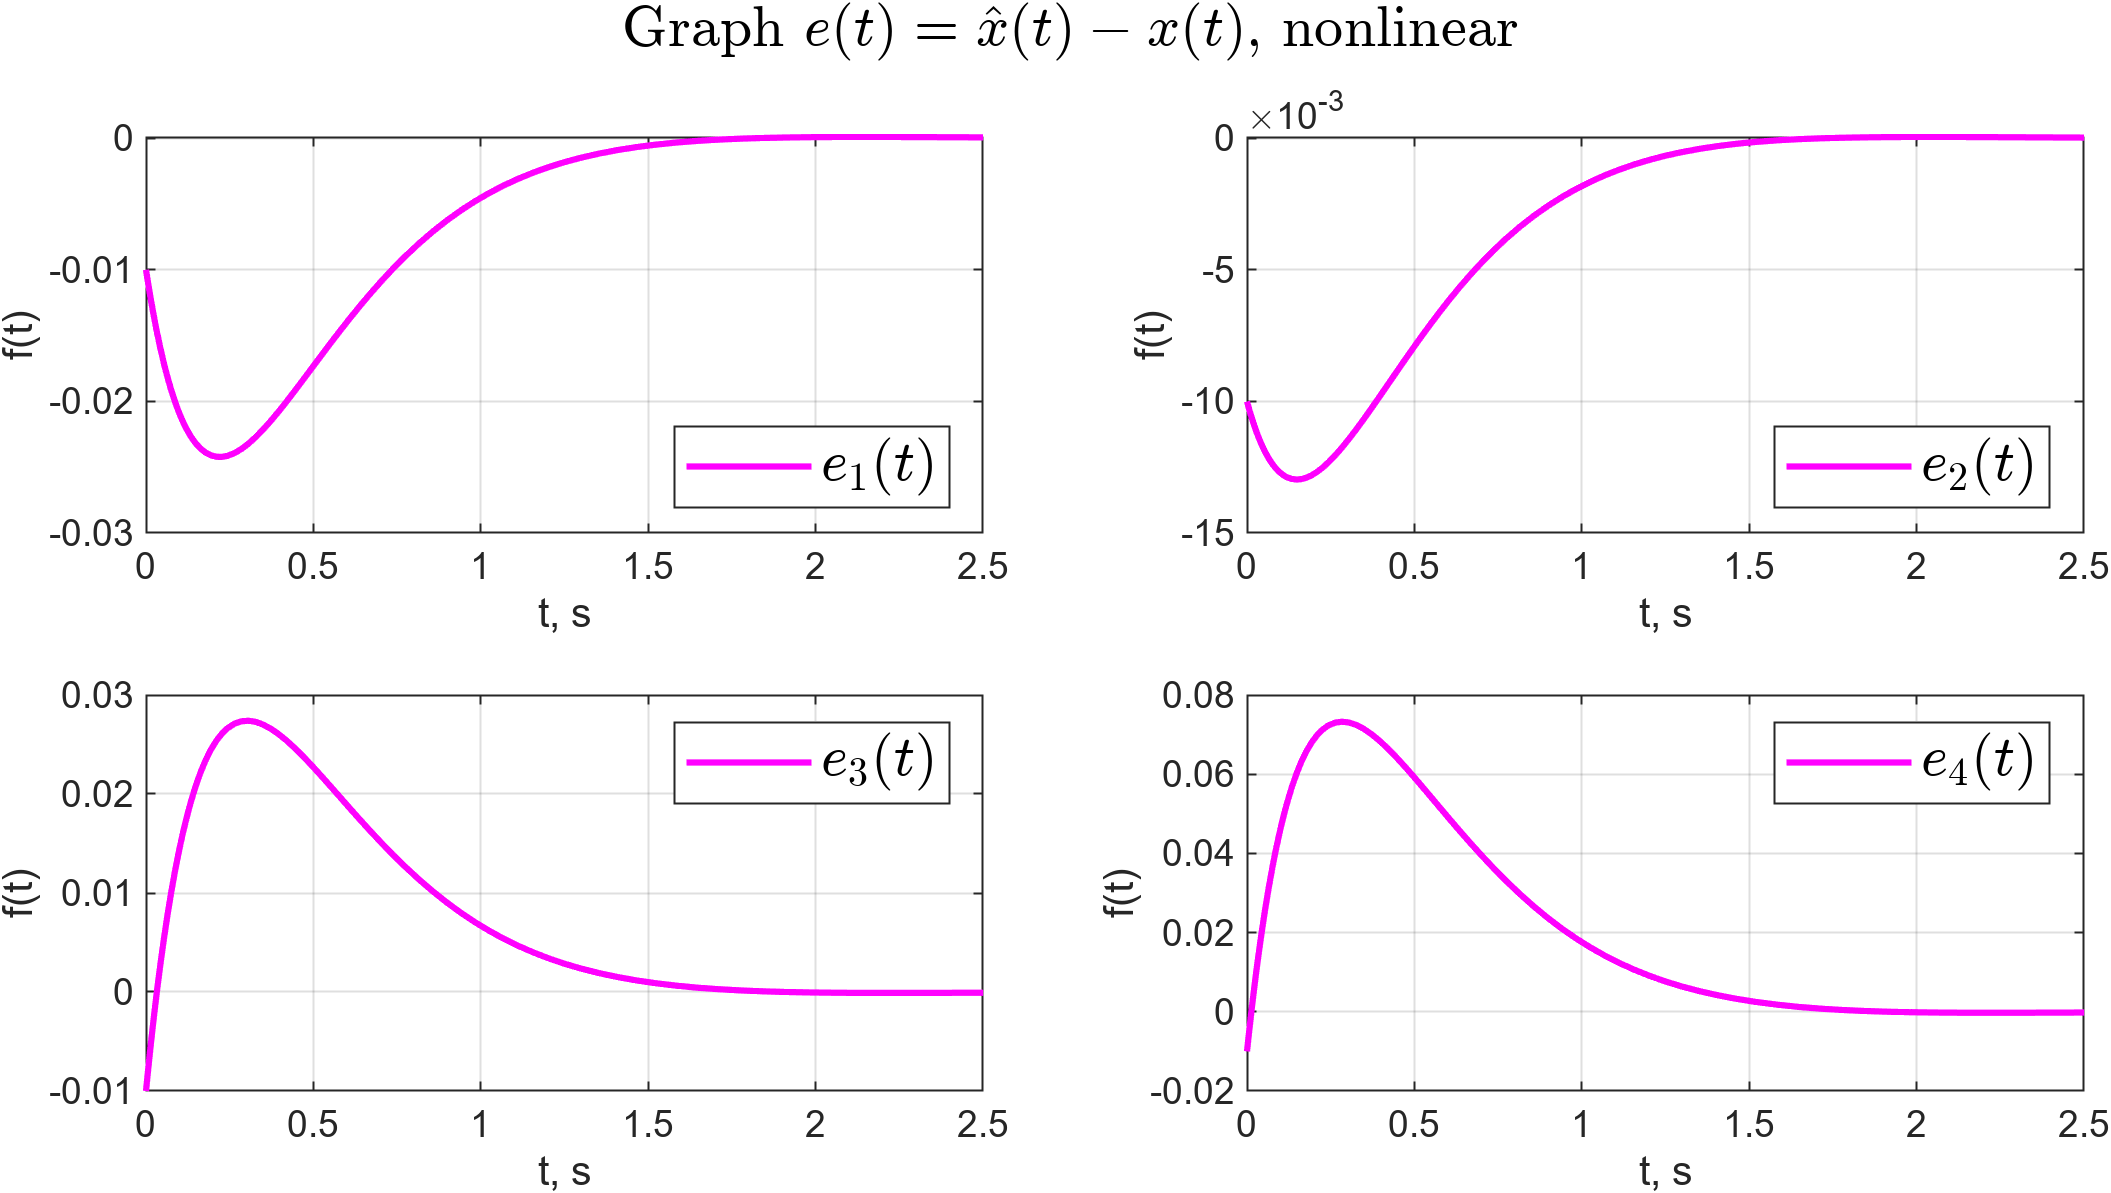
\includegraphics[width=1\linewidth]{pic/3_e_nlin_02_L1.png}}
\caption{Графики $e (t) =\hat{x}(t) - x(t)$.}
\label{3_e_nlin_02_L1}
\end{figure}

Теперь зададимся несколькими дополнительными наборами собственных чисел наблюдателя и исследуем их влияние на систему

\begin{equation*}
  \begin{matrix}
      \sigma_1 = \{ -0.1, -0.2, -0.3, -0.4 \}, & \sigma_2 = \{ -5, -10, -15, -20 \},\\
      \sigma_3 = \{ -1, -2, -3 \pm 3i \} & 
 \end{matrix}
\end{equation*}

\begin{figure}[!h]
\center{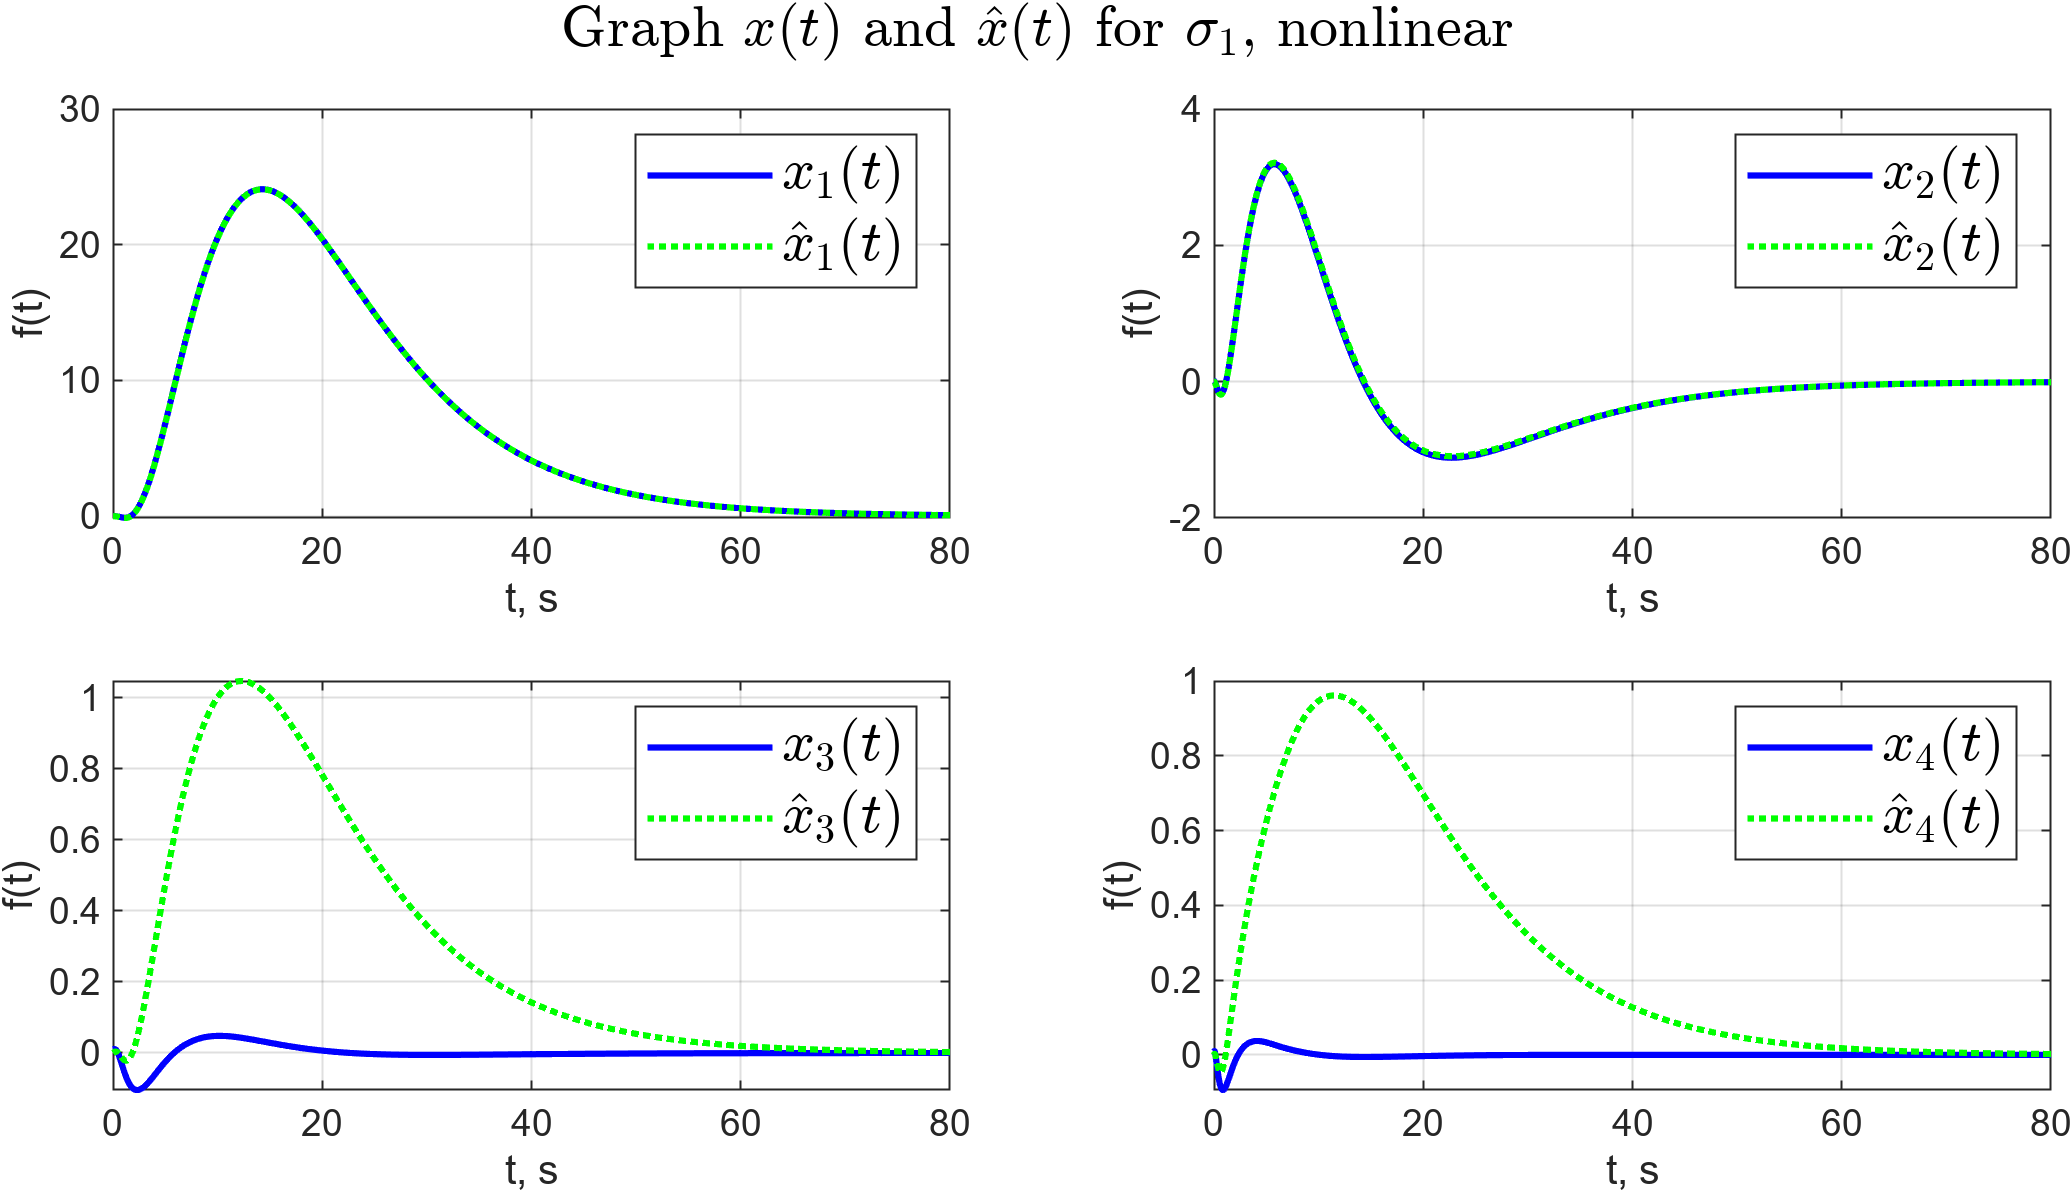
\includegraphics[width=1\linewidth]{pic/3_xx_nlin_02_L2.png}}
\caption{Графики $x(t)$ и $\hat{x}(t)$ для $ \sigma_1 = \{ -0.1, -0.2, -0.3, -0.4 \}$.}
\label{3_xx_nlin_02_L2}
\end{figure}


\begin{figure}[!h]
\center{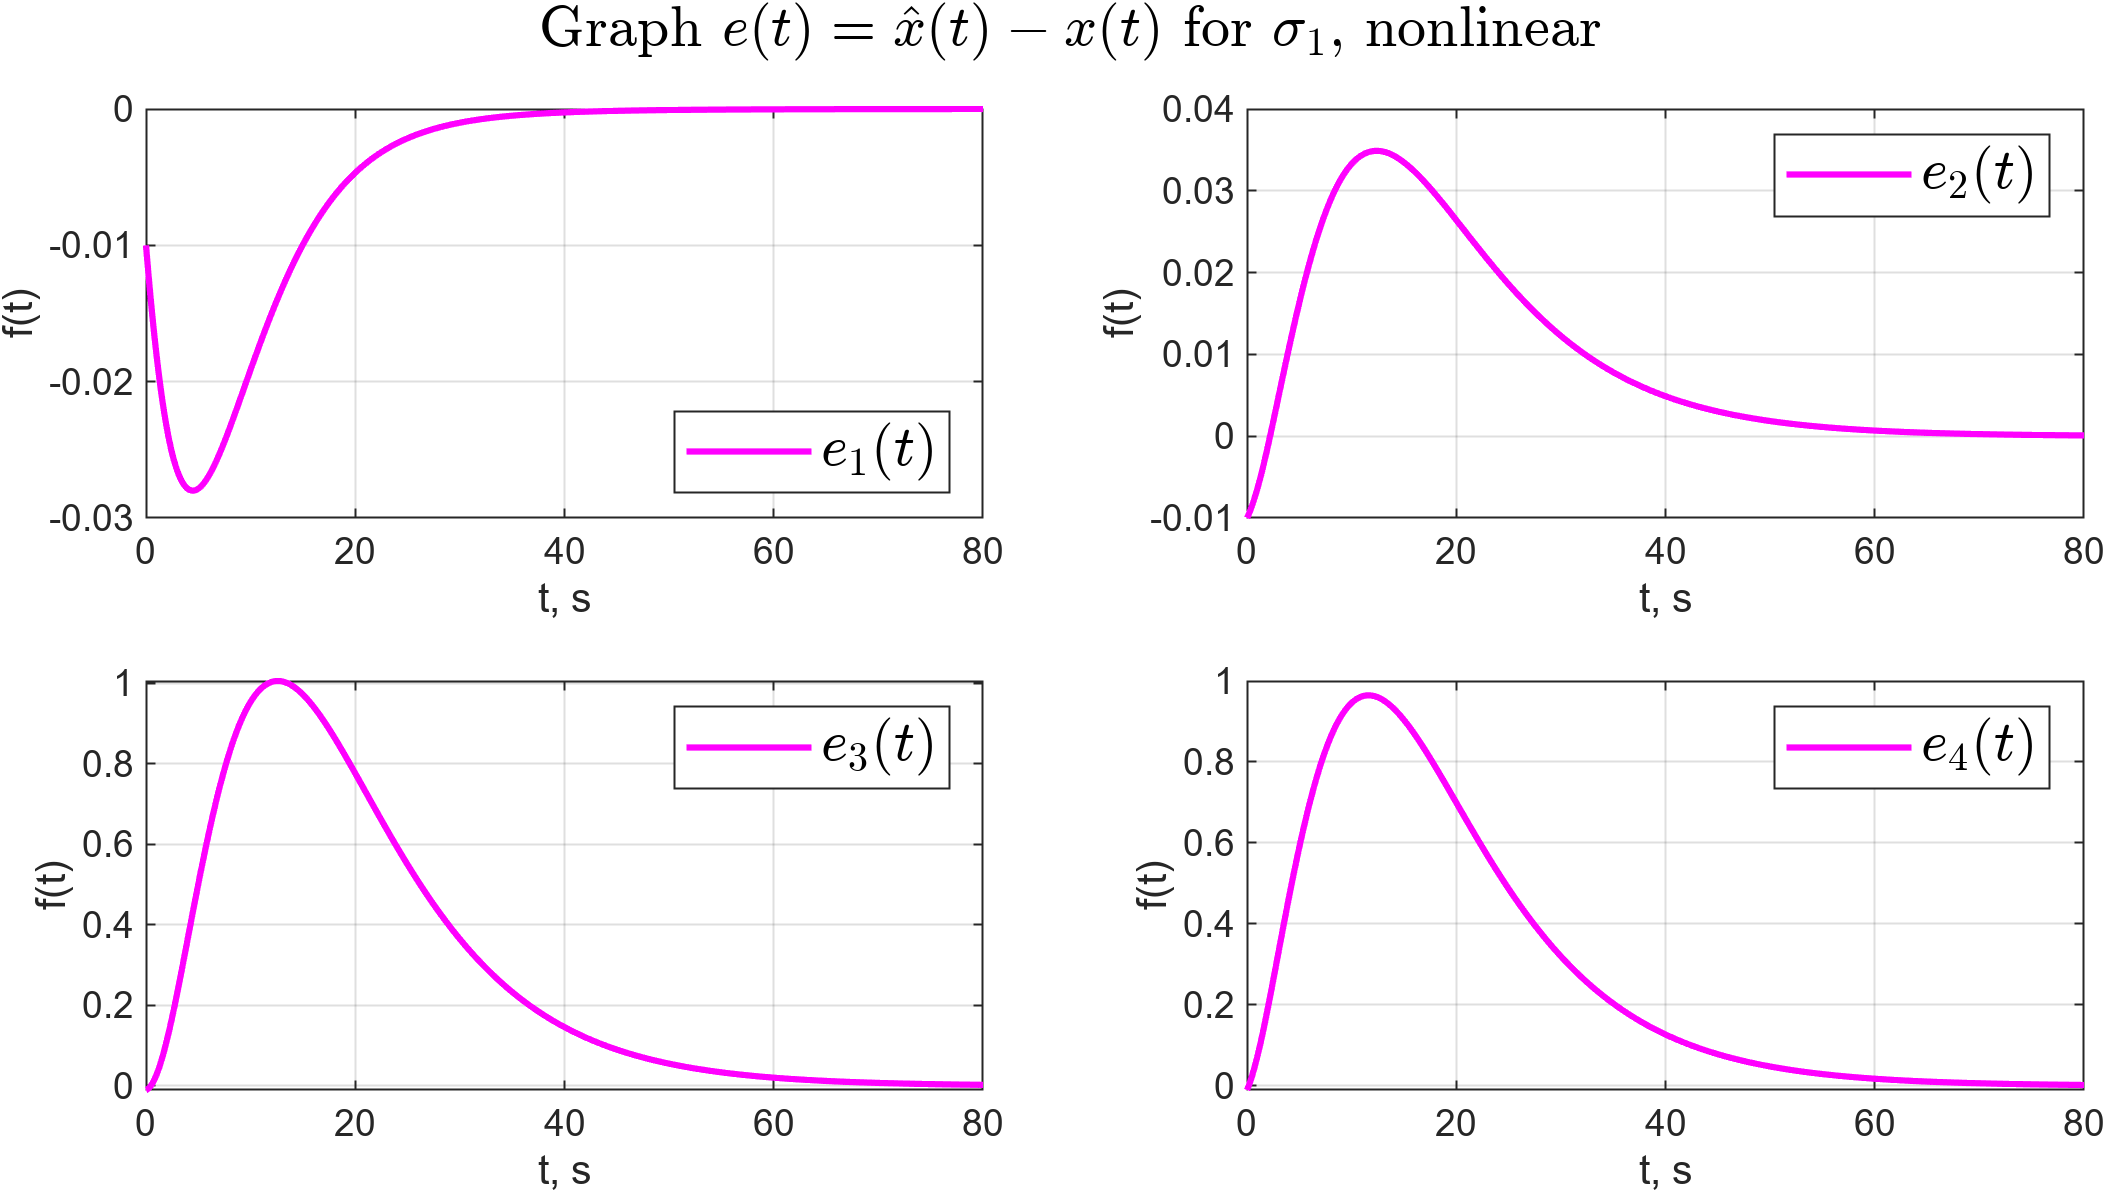
\includegraphics[width=1\linewidth]{pic/3_e_nlin_02_L2.png}}
\caption{Графики $e (t) =\hat{x}(t) - x(t)$ для $ \sigma_1 = \{ -0.1, -0.2, -0.3, -0.4 \}$.}
\label{3_e_nlin_02_L2}
\end{figure}

При малых значениях спектра наблюдателя  $ \sigma_1 = \{ -0.1, -0.2, -0.3, -0.4 \}$ наблюдатель выполняет свою задачу (рисунки \ref{3_xx_nlin_02_L2} и \ref{3_e_nlin_02_L2}), время, за которое ошибка наблюдения сходится к нулю сильно возрастает (до $\approx 80$ с).



\begin{figure}[!h]
\center{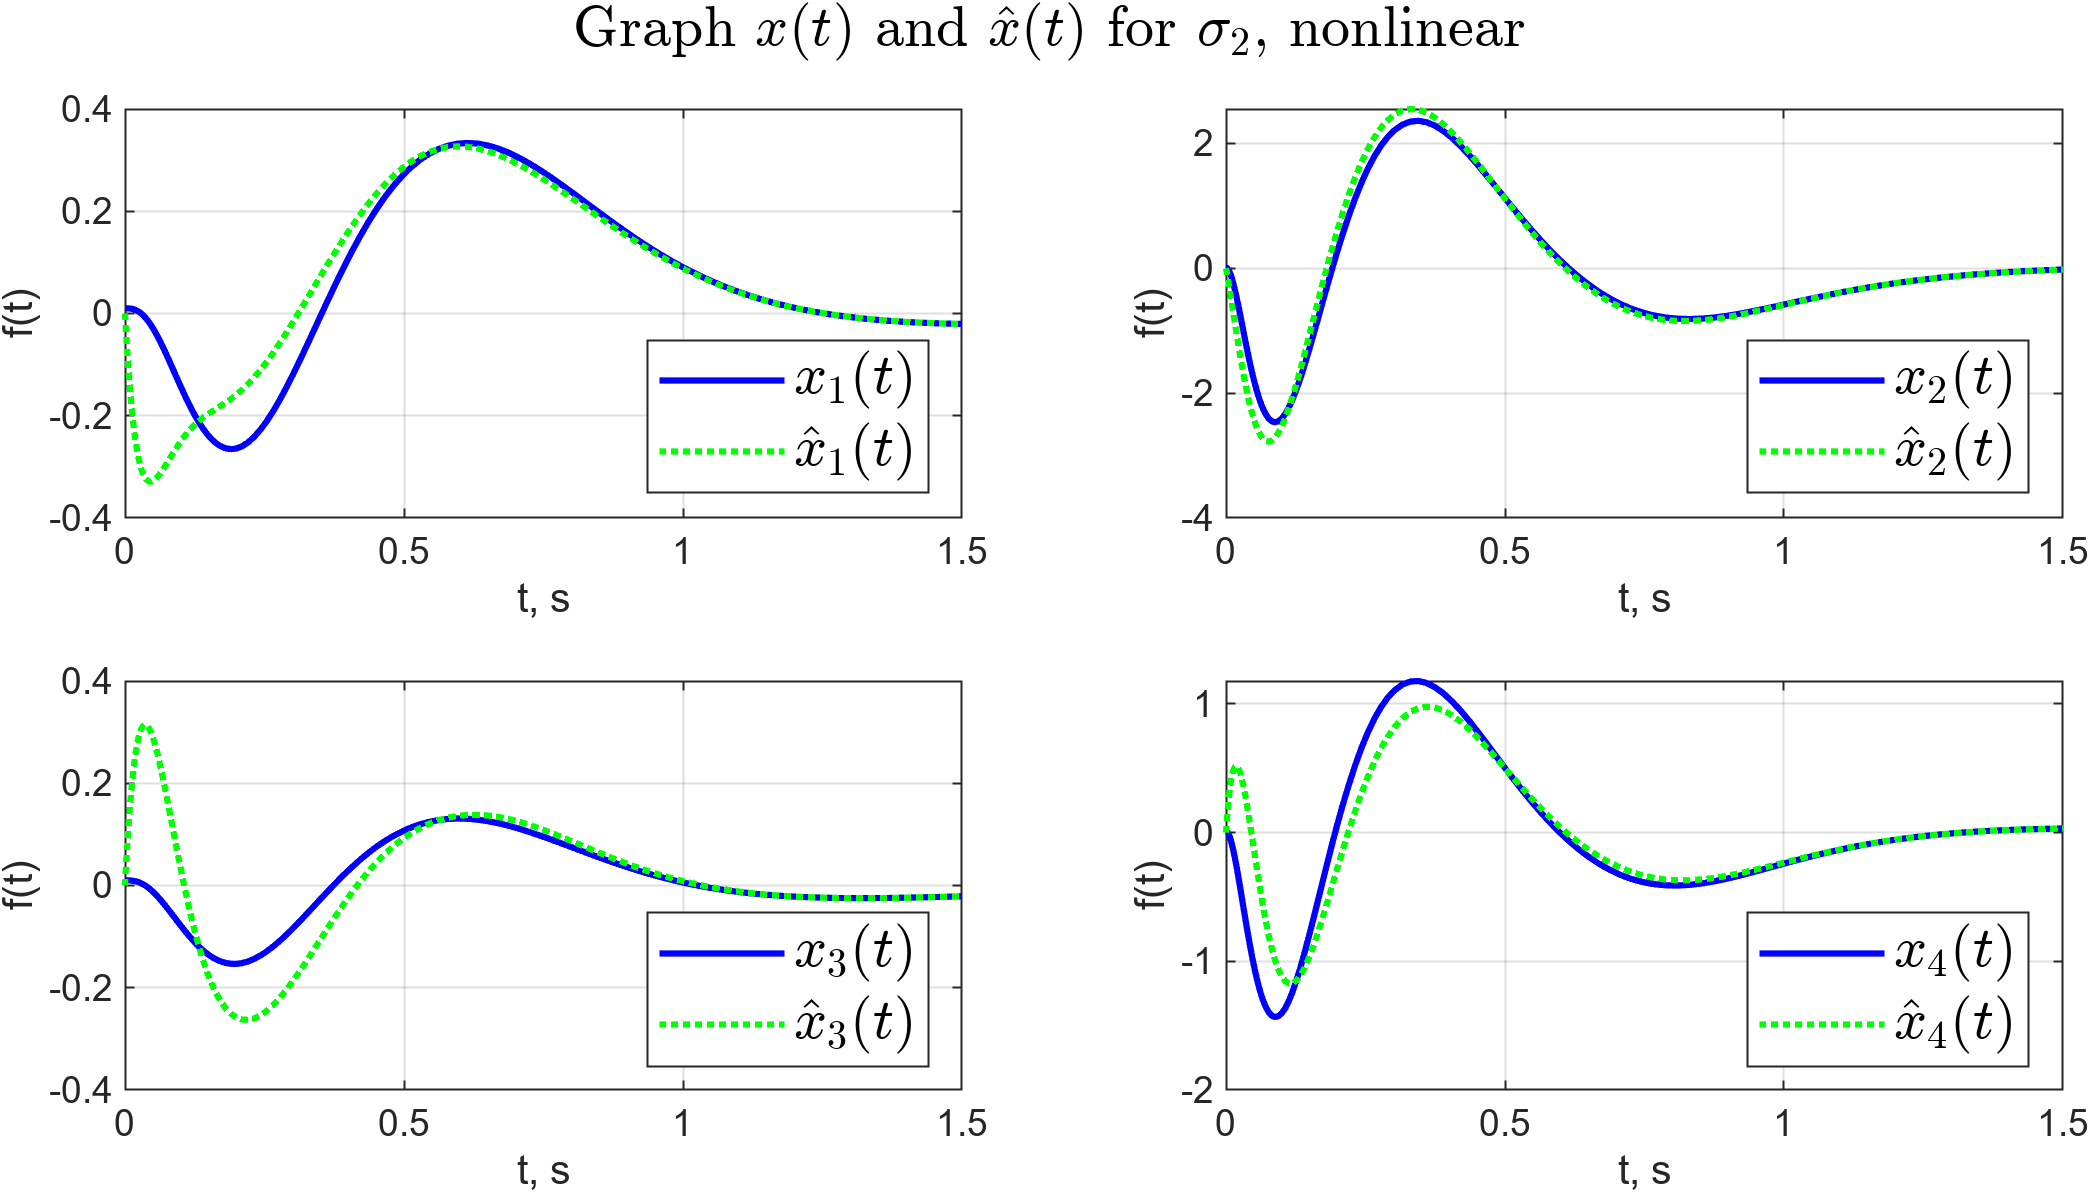
\includegraphics[width=1\linewidth]{pic/3_xx_nlin_02_L3.png}}
\caption{Графики $x(t)$ и $\hat{x}(t)$ для $ \sigma_2 = \{ -5, -10, -15, -20 \}$.}
\label{3_xx_nlin_02_L3}
\end{figure}


\begin{figure}[!h]
\center{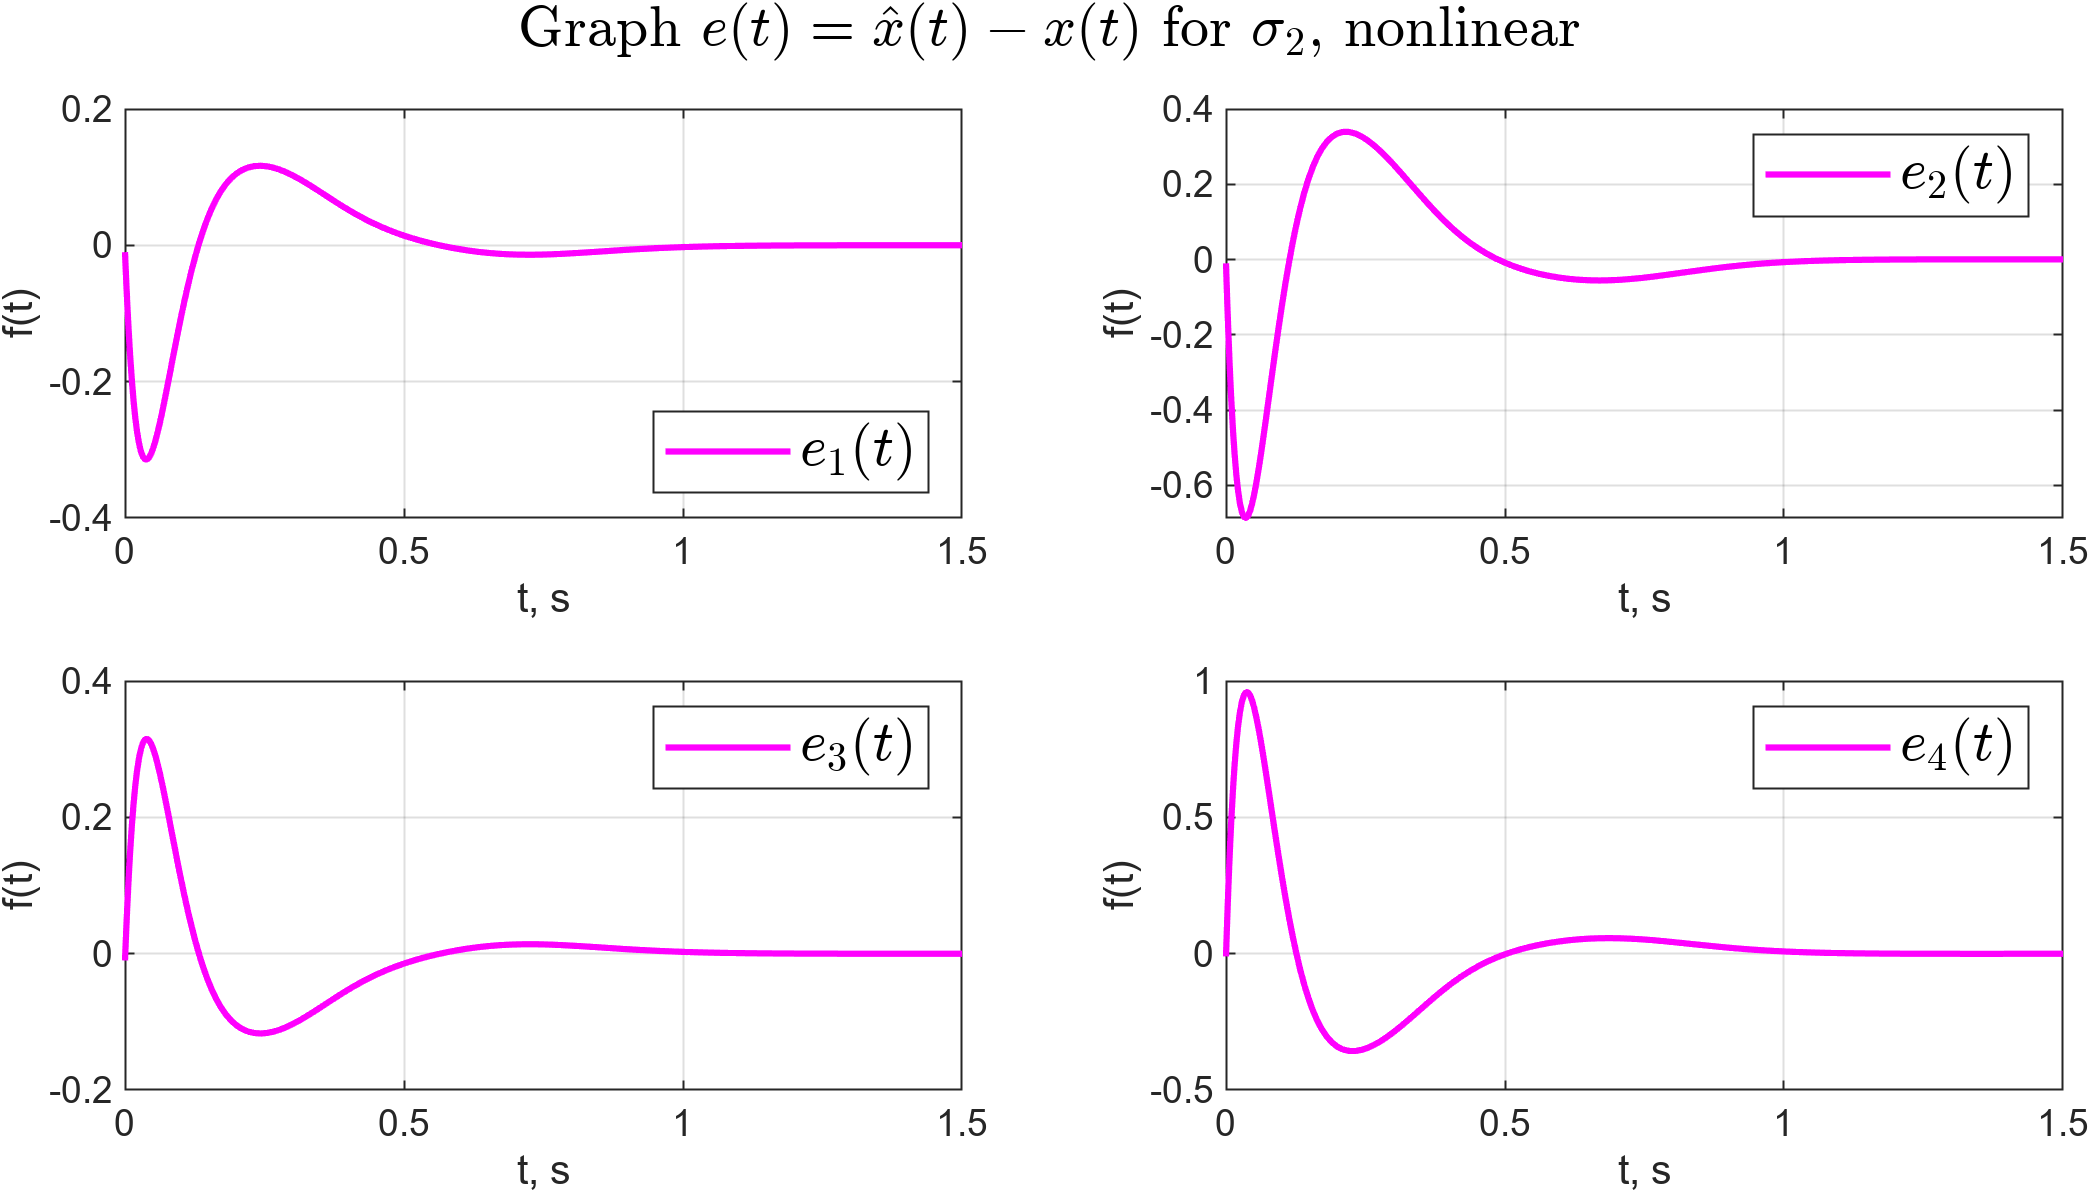
\includegraphics[width=1\linewidth]{pic/3_e_nlin_02_L3.png}}
\caption{Графики $e (t) =\hat{x}(t) - x(t)$ для $ \sigma_2 = \{ -5, -10, -15, -20 \}$.}
\label{3_e_nlin_02_L3}
\end{figure}

При больших значениях собственных чисел наблюдателя $ \sigma_1 = \{ -5, -10, -15, -20 \}$ время, после которого ошибка наблюдения становится неотличима от нуля, существенно сокращается до $\approx 1$ секунды. 

\begin{figure}[!h]
\center{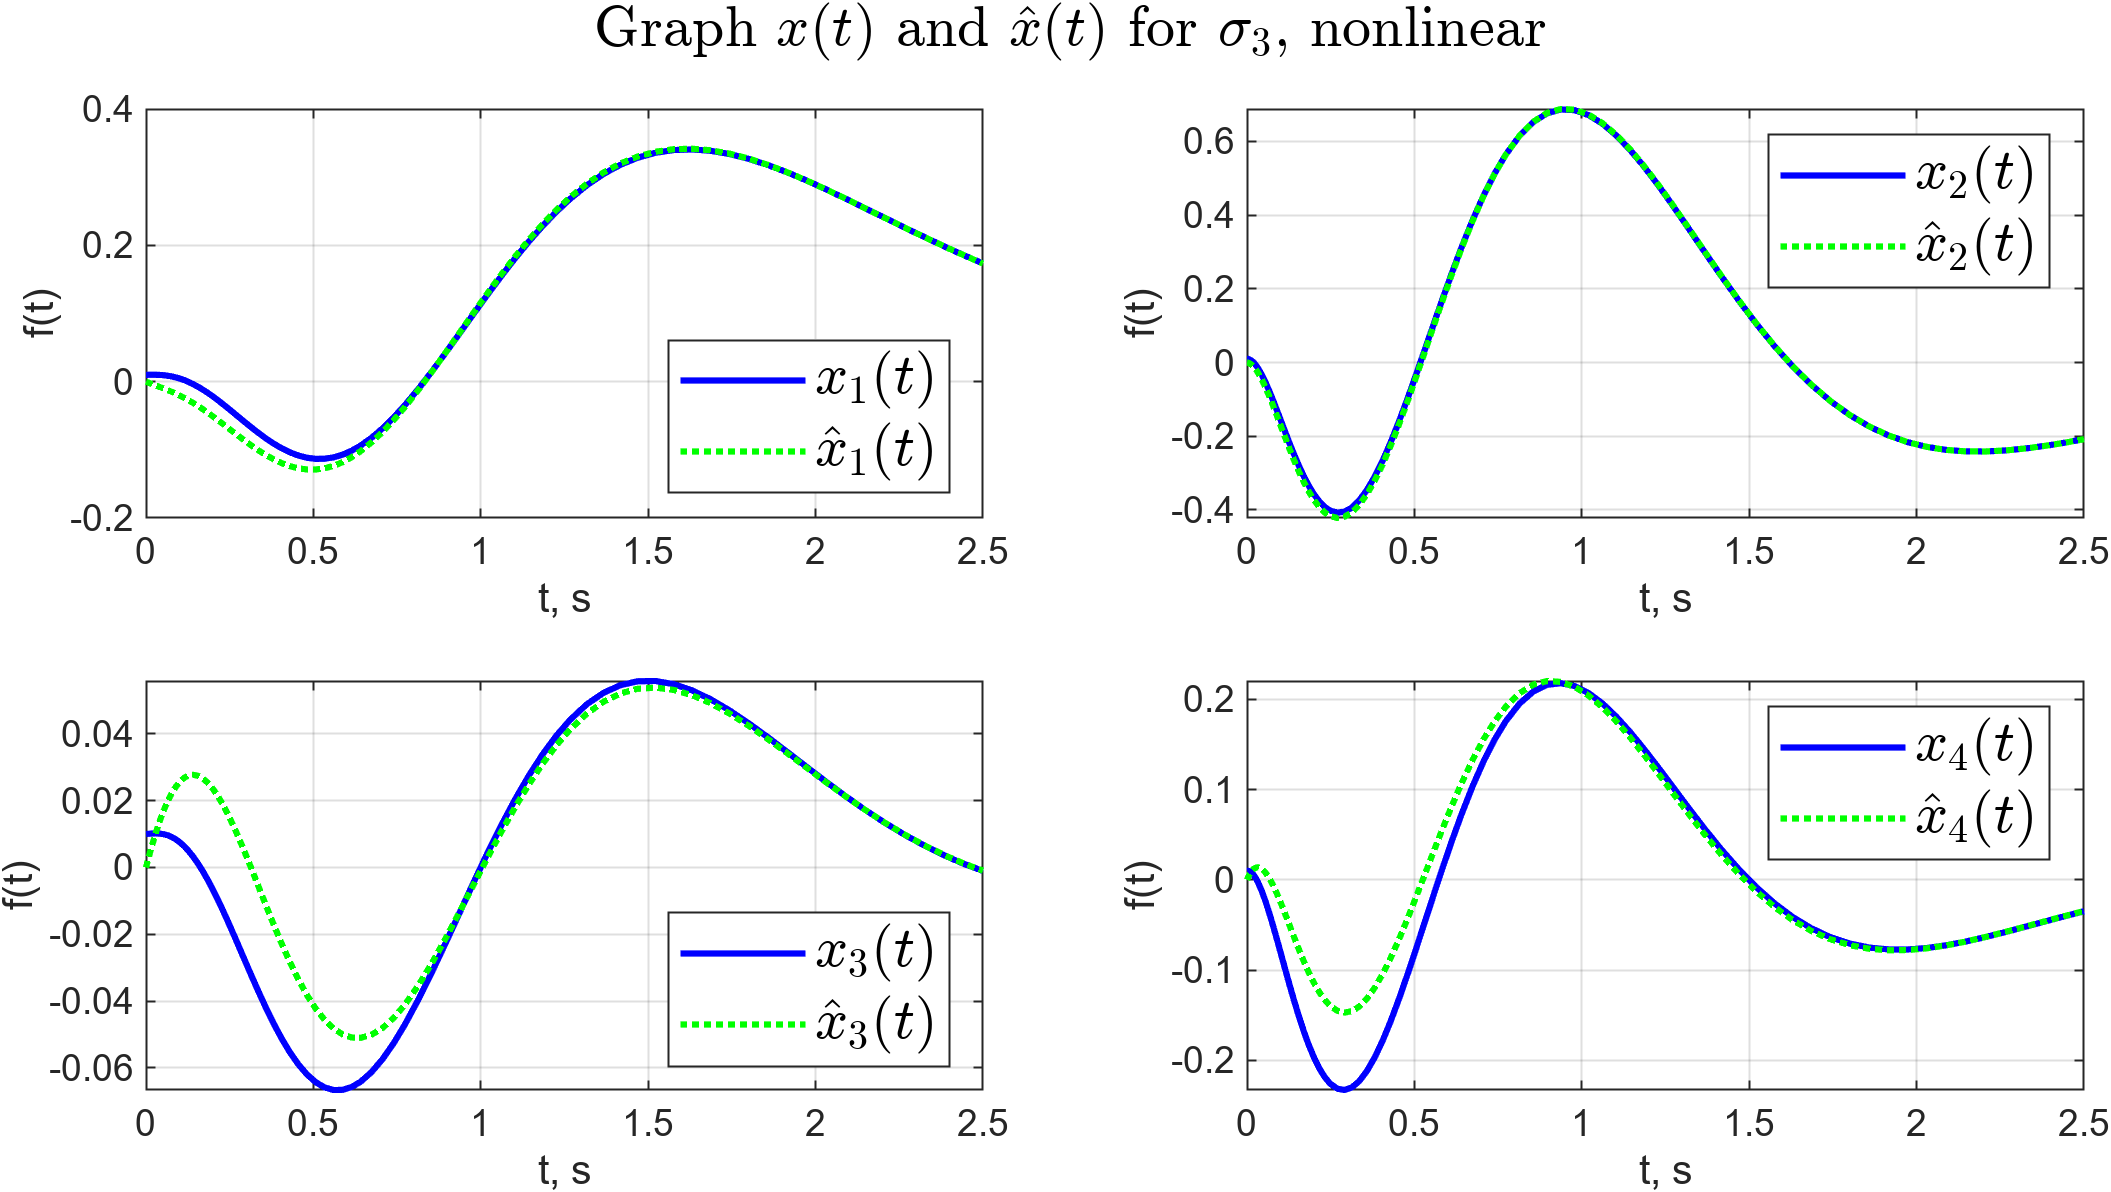
\includegraphics[width=1\linewidth]{pic/3_xx_nlin_02_L4.png}}
\caption{Графики $x(t)$ и $\hat{x}(t)$ для $ \sigma_3 = \{ -1, -2, -3 \pm 3i \}$.}
\label{3_xx_nlin_02_L4}
\end{figure}


\begin{figure}[!h]
\center{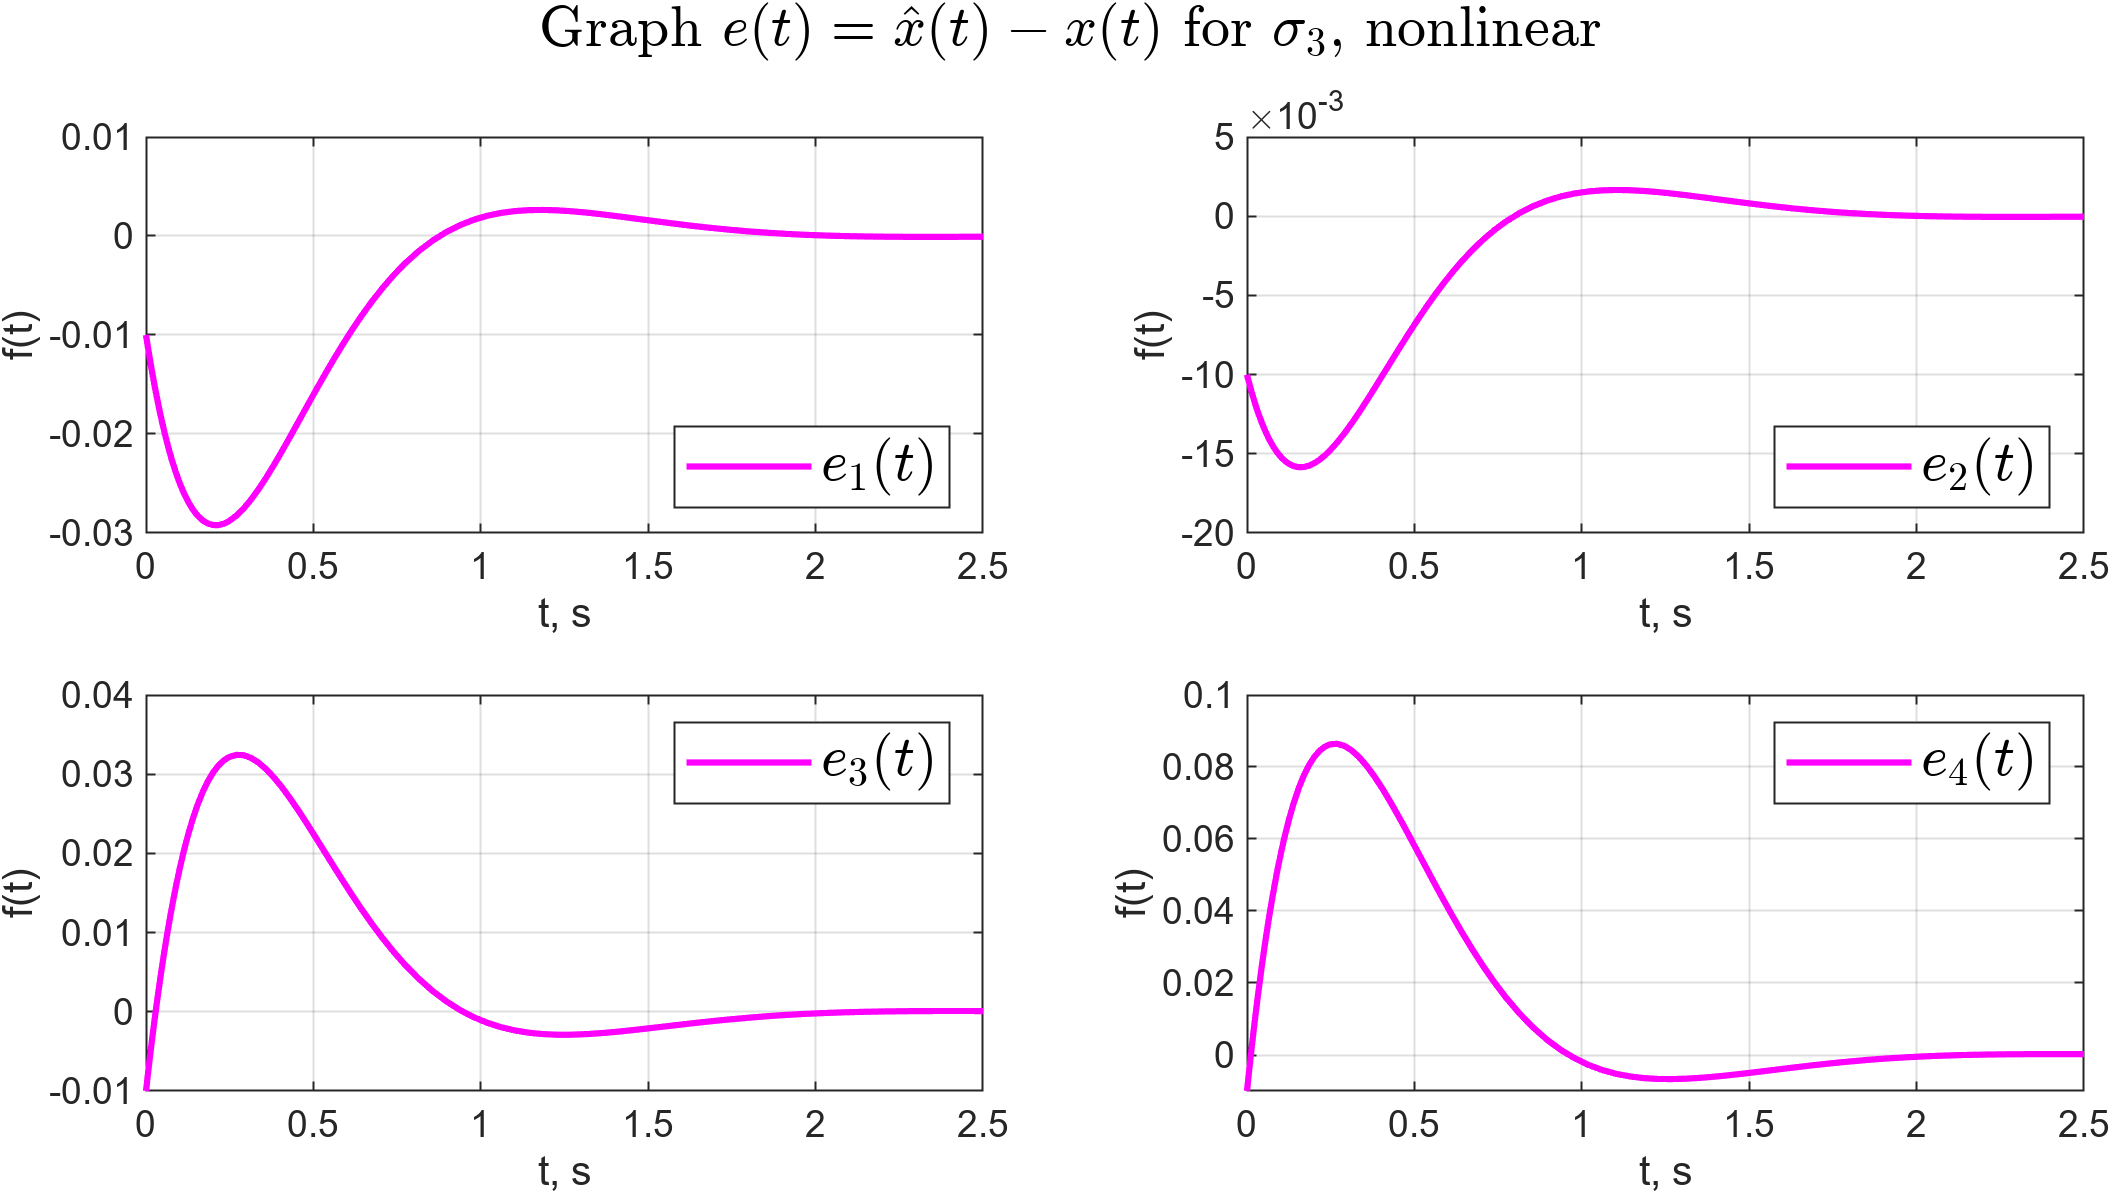
\includegraphics[width=1\linewidth]{pic/3_e_nlin_02_L4.png}}
\caption{Графики $e (t) =\hat{x}(t) - x(t)$ для $ \sigma_3 = \{ -1, -2, -3 \pm 3i \}$.}
\label{3_e_nlin_02_L4}
\end{figure}


\newpage
\subsection{Наблюдатель пониженной размерности}
Запишем уравнения наблюдателя пониженного порядка

\begin{equation}
    \begin{cases}
        \dot{\hat{z}} = \Gamma \hat{z} - Yy+QBu,\\
        \hat{x} = \begin{bmatrix}
            C\\Q
        \end{bmatrix}^{-1} \begin{bmatrix}
            y\\
            \hat{z}
        \end{bmatrix}
    \end{cases}
\end{equation}

Зададимся желаемым спектром матрицы наблюдателя пониженного порядка $\sigma (\Gamma) = \{ -1, \, \, -2 \}$. Запишем матрицы $\Gamma$ и $Y$

\begin{equation}
    \Gamma = \begin{bmatrix}
        -1 & 0\\
        0 & -2
    \end{bmatrix}, \, \, 
    Y = \begin{bmatrix}
        1 & 1\\
        1 & 1
    \end{bmatrix}
\end{equation}

Синтезируем матрицу преобразования $Q$ на основании выбранного желаемого спектра $\sigma (\Gamma)$. Решим уравнение Сильвестра

\begin{equation}
    \Gamma Q - Q A = YC
\end{equation}
относительно $Q$ и получим

\begin{equation}
    Q = \begin{bmatrix}
        -1&	1&	0.2589	&-0.2589\\
-0.5&	0.25&1.156&-0.578
    \end{bmatrix}
\end{equation}

Зададимся начальными условиями  системы и наблюдателя

\begin{equation}
    \begin{matrix}
        x(0) = \begin{bmatrix}
    0.01&&
    0.01&&
    0.01&&
    0.01
\end{bmatrix}^T\\
 \hat{z}(0) = \begin{bmatrix}
    0&&
    0
\end{bmatrix}^T
    \end{matrix}
\end{equation}

И выполним моделирование для той же замкнутой системы со спектром $\sigma = \{ -3, -2.5, -2, -1.5 \}$, что и для наблюдателя полной размерности

\begin{figure}[!h]
\center{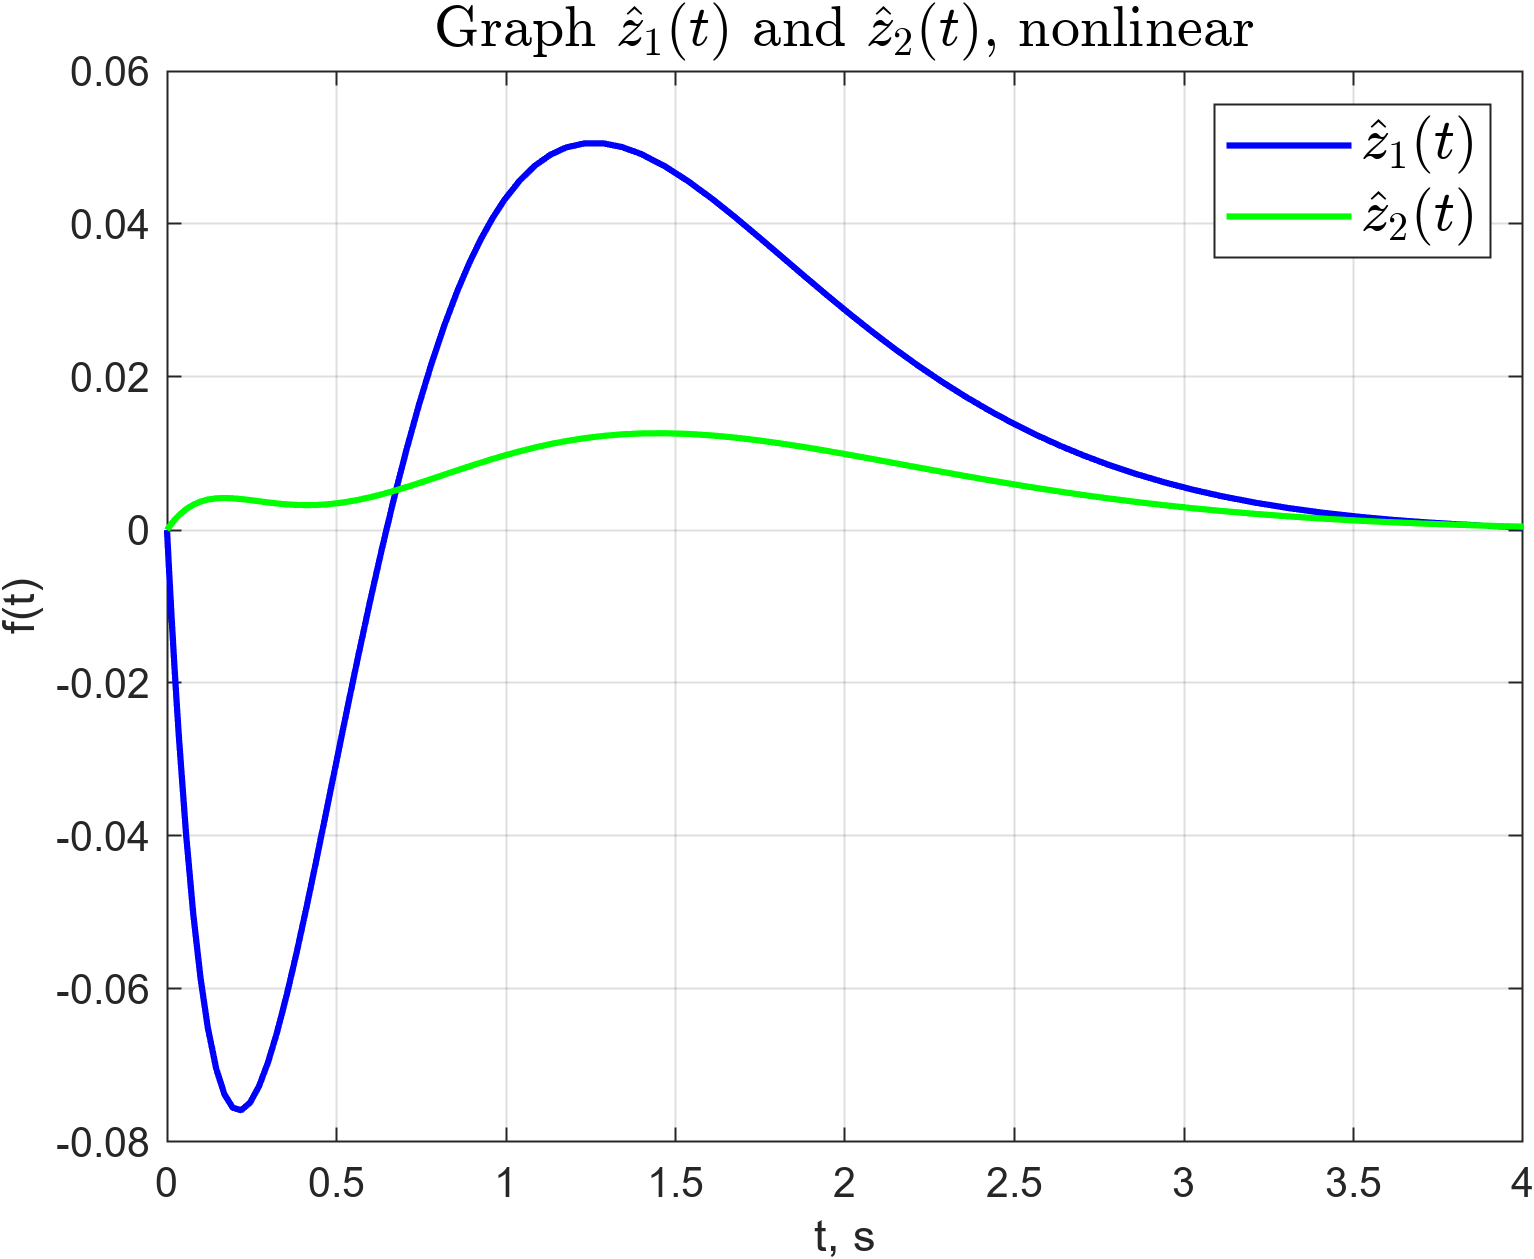
\includegraphics[width=0.6\linewidth]{pic/3_z_nlin_02_LW1.png}}
\caption{График $\hat{z}(t)$ для $ \sigma (\Gamma) = \{ -1, -2 \}$.}
\label{3_z_nlin_02_LW1}
\end{figure}

\begin{figure}[!h]
\center{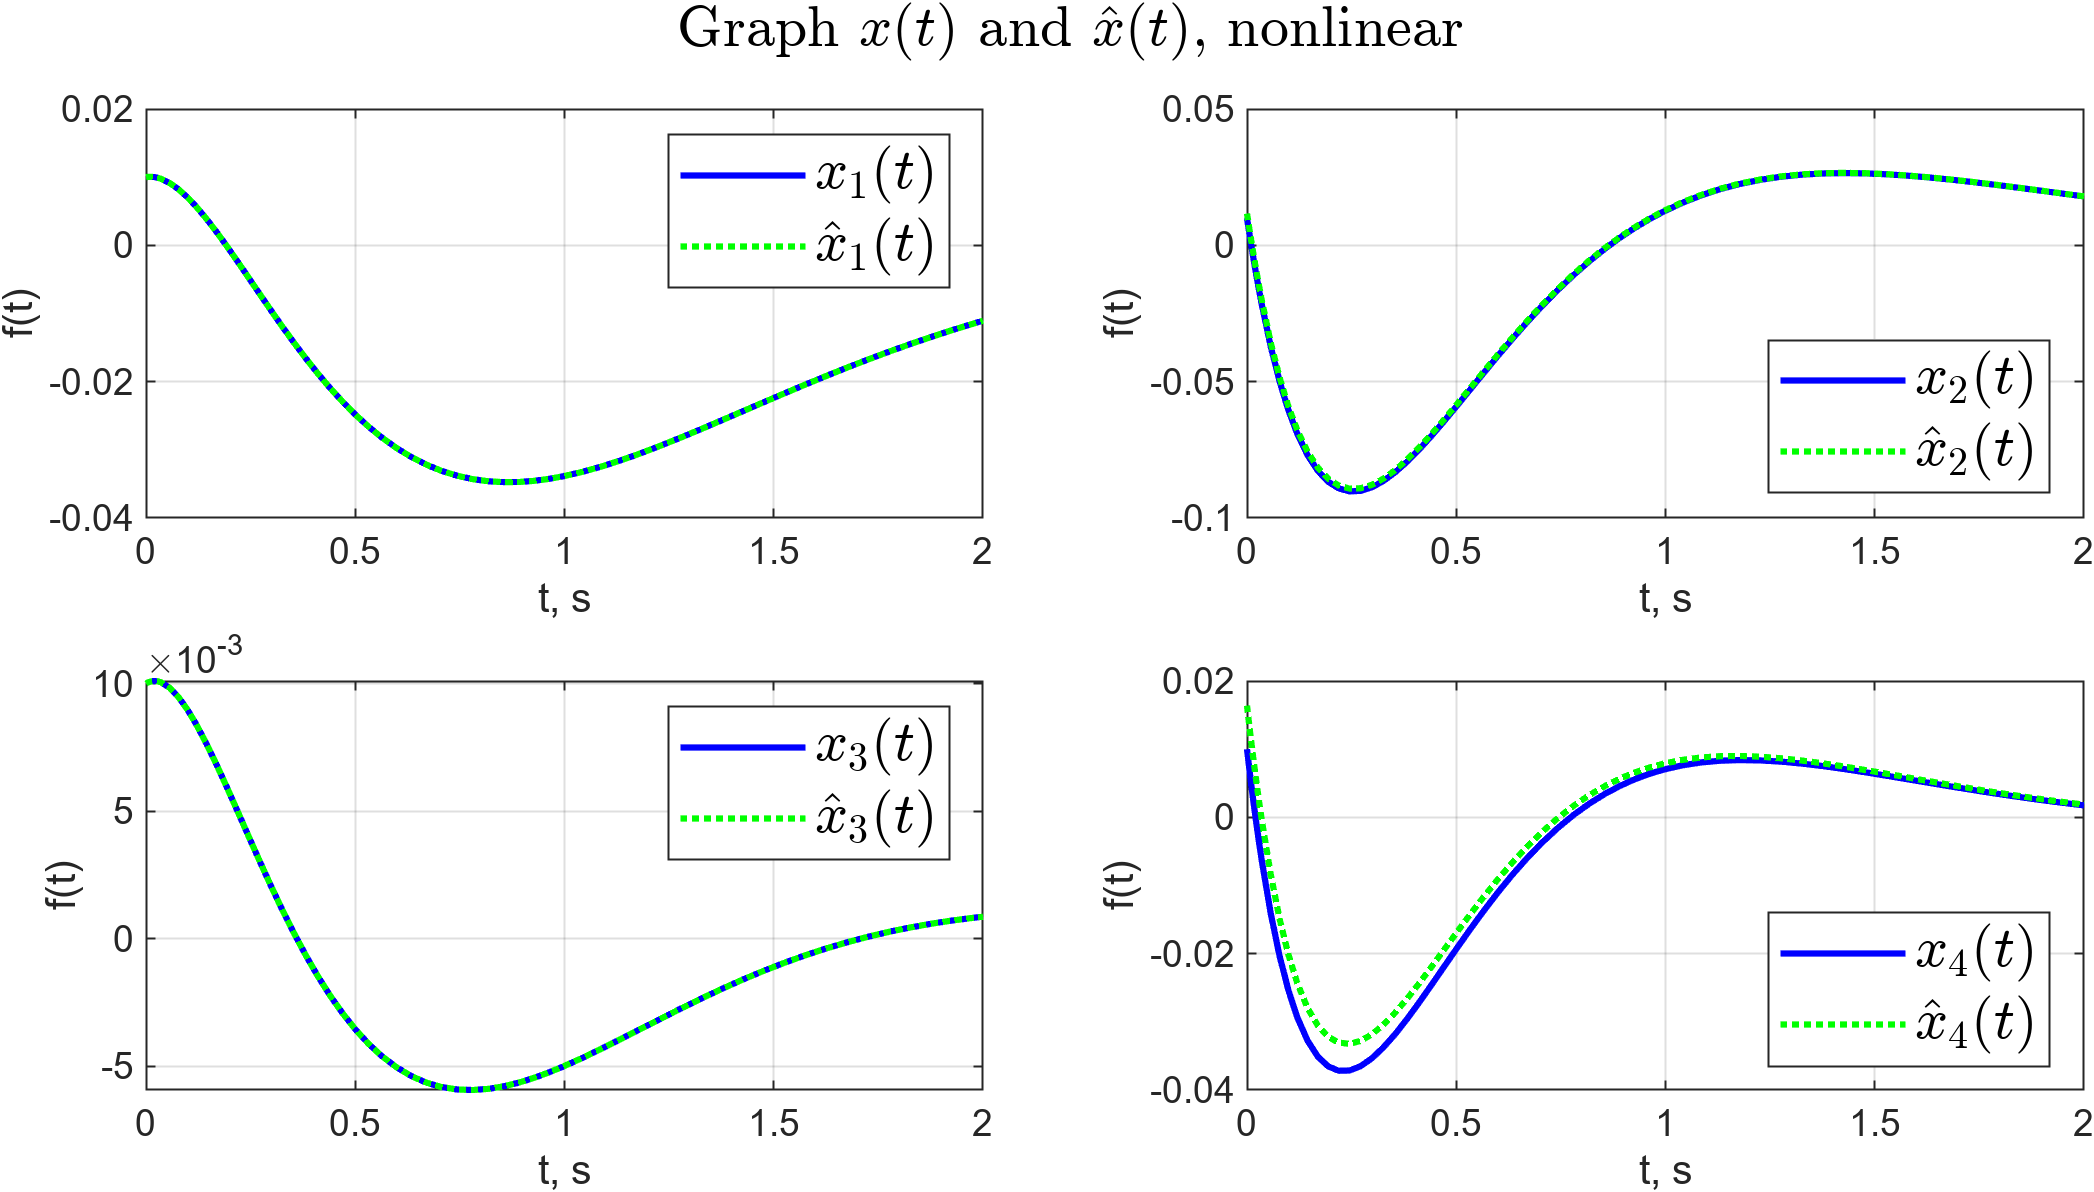
\includegraphics[width=1\linewidth]{pic/3_xx_nlin_02_LW1.png}}
\caption{Графики $x(t)$ и $\hat{x}(t)$ для $ \sigma (\Gamma) = \{ -1, -2 \}$.}
\label{3_xx_nlin_02_LW1}
\end{figure}


\begin{figure}[!h]
\center{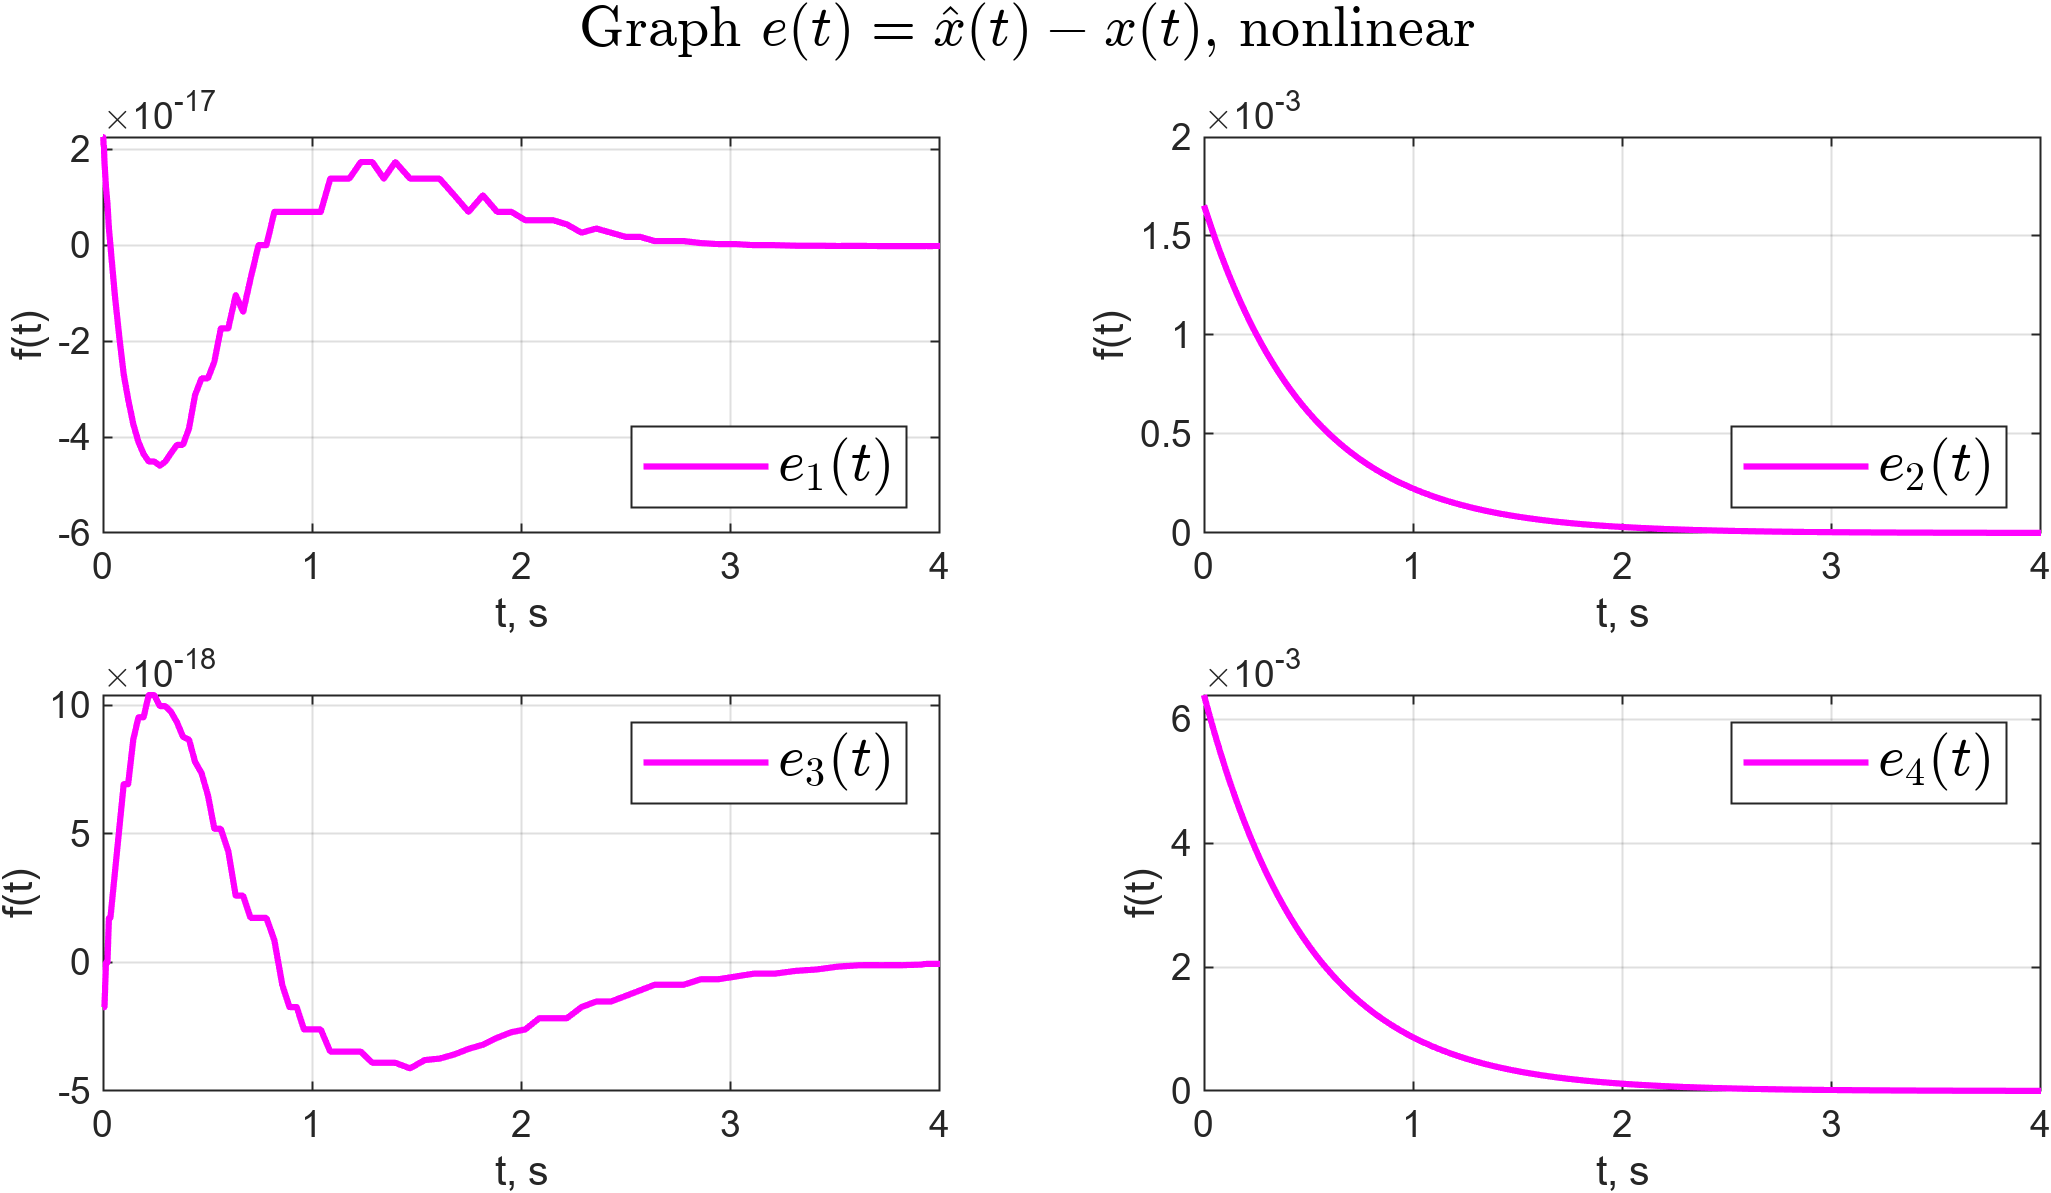
\includegraphics[width=1\linewidth]{pic/3_e_nlin_02_LW1.png}}
\caption{Графики $e (t) =\hat{x}(t) - x(t)$ для $ \sigma (\Gamma) = \{ -1, -2 \}$.}
\label{3_e_nlin_02_LW1}
\end{figure}

Рассмотрим работу наблюдателя пониженной размерности при значениях спектра 

\begin{equation*}
  \begin{matrix}
      \sigma_1 = \{ -0.1, -0.2 \}, & \sigma_2 = \{ -10, -20 \},\\
      \sigma_3 = \{ -2  \pm i \} & 
 \end{matrix}
\end{equation*}

\begin{figure}[!h]
\center{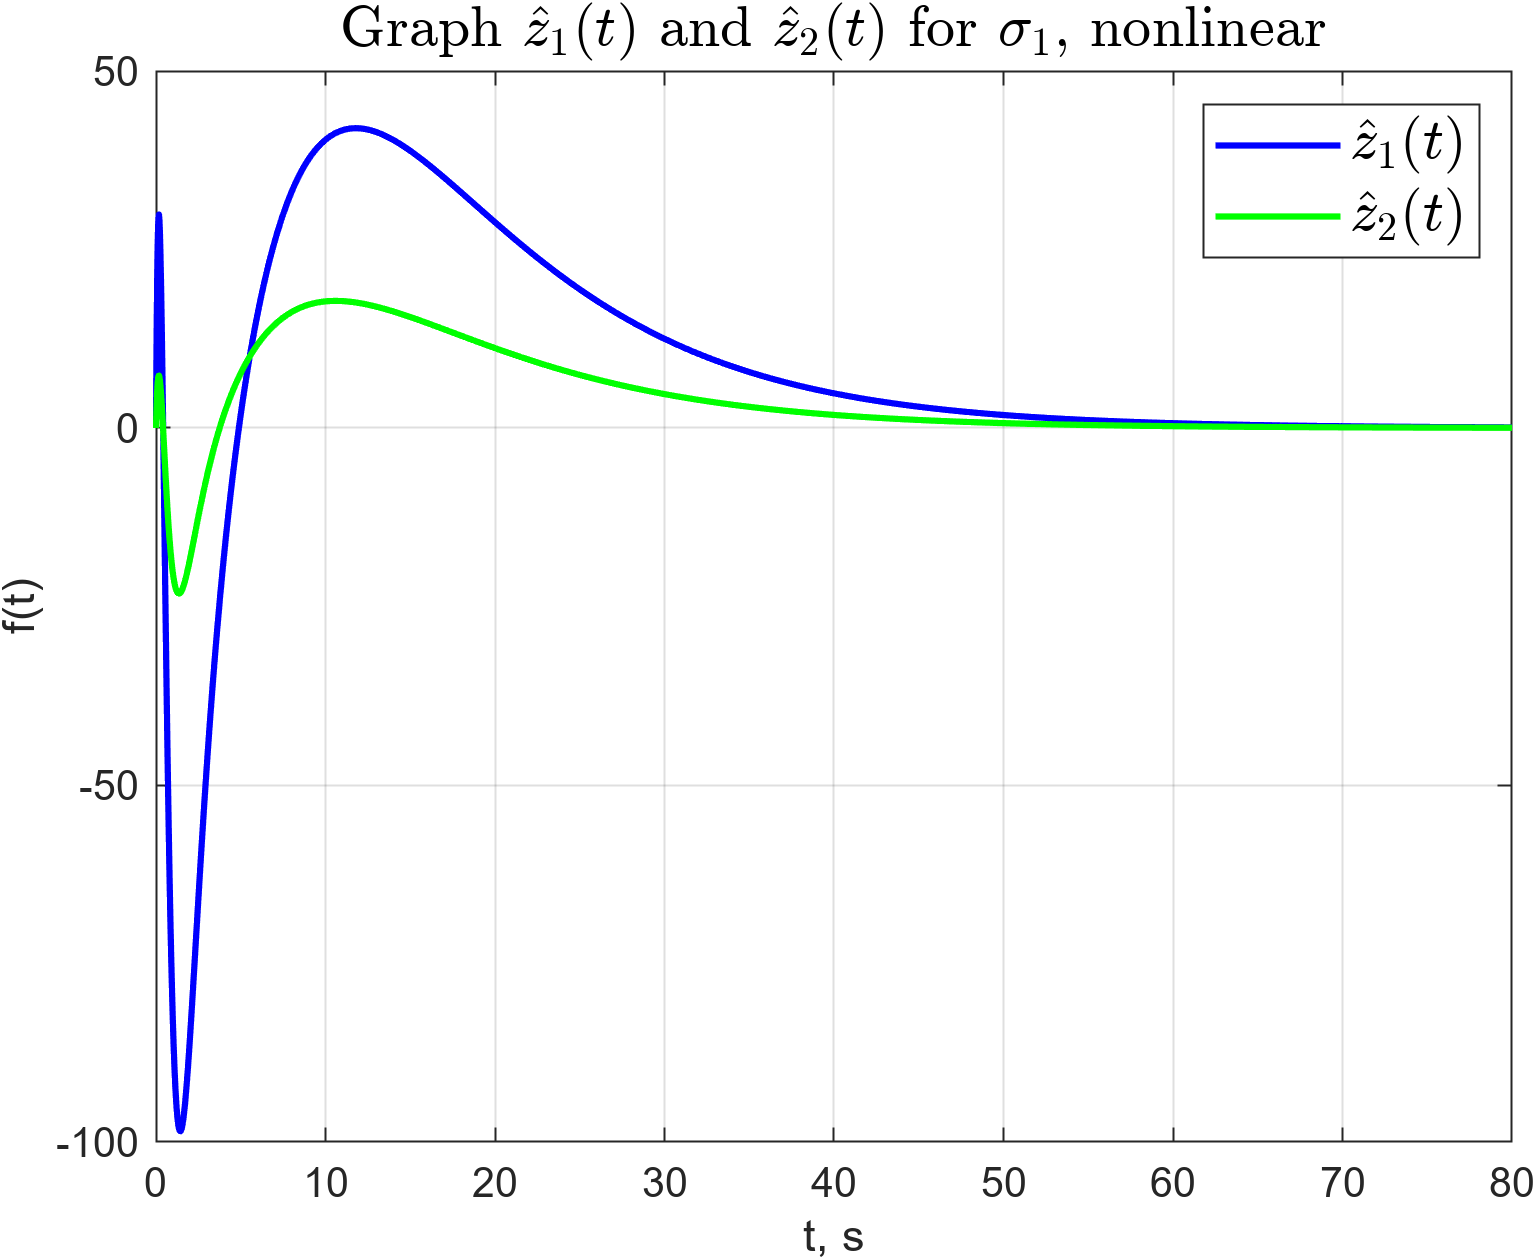
\includegraphics[width=0.6\linewidth]{pic/3_z_nlin_02_LW2.png}}
\caption{График $\hat{z}(t)$ для $ \sigma_1 (\Gamma) = \{ -0.1, -0.2 \}$.}
\label{3_z_nlin_02_LW2}
\end{figure}

\begin{figure}[!h]
\center{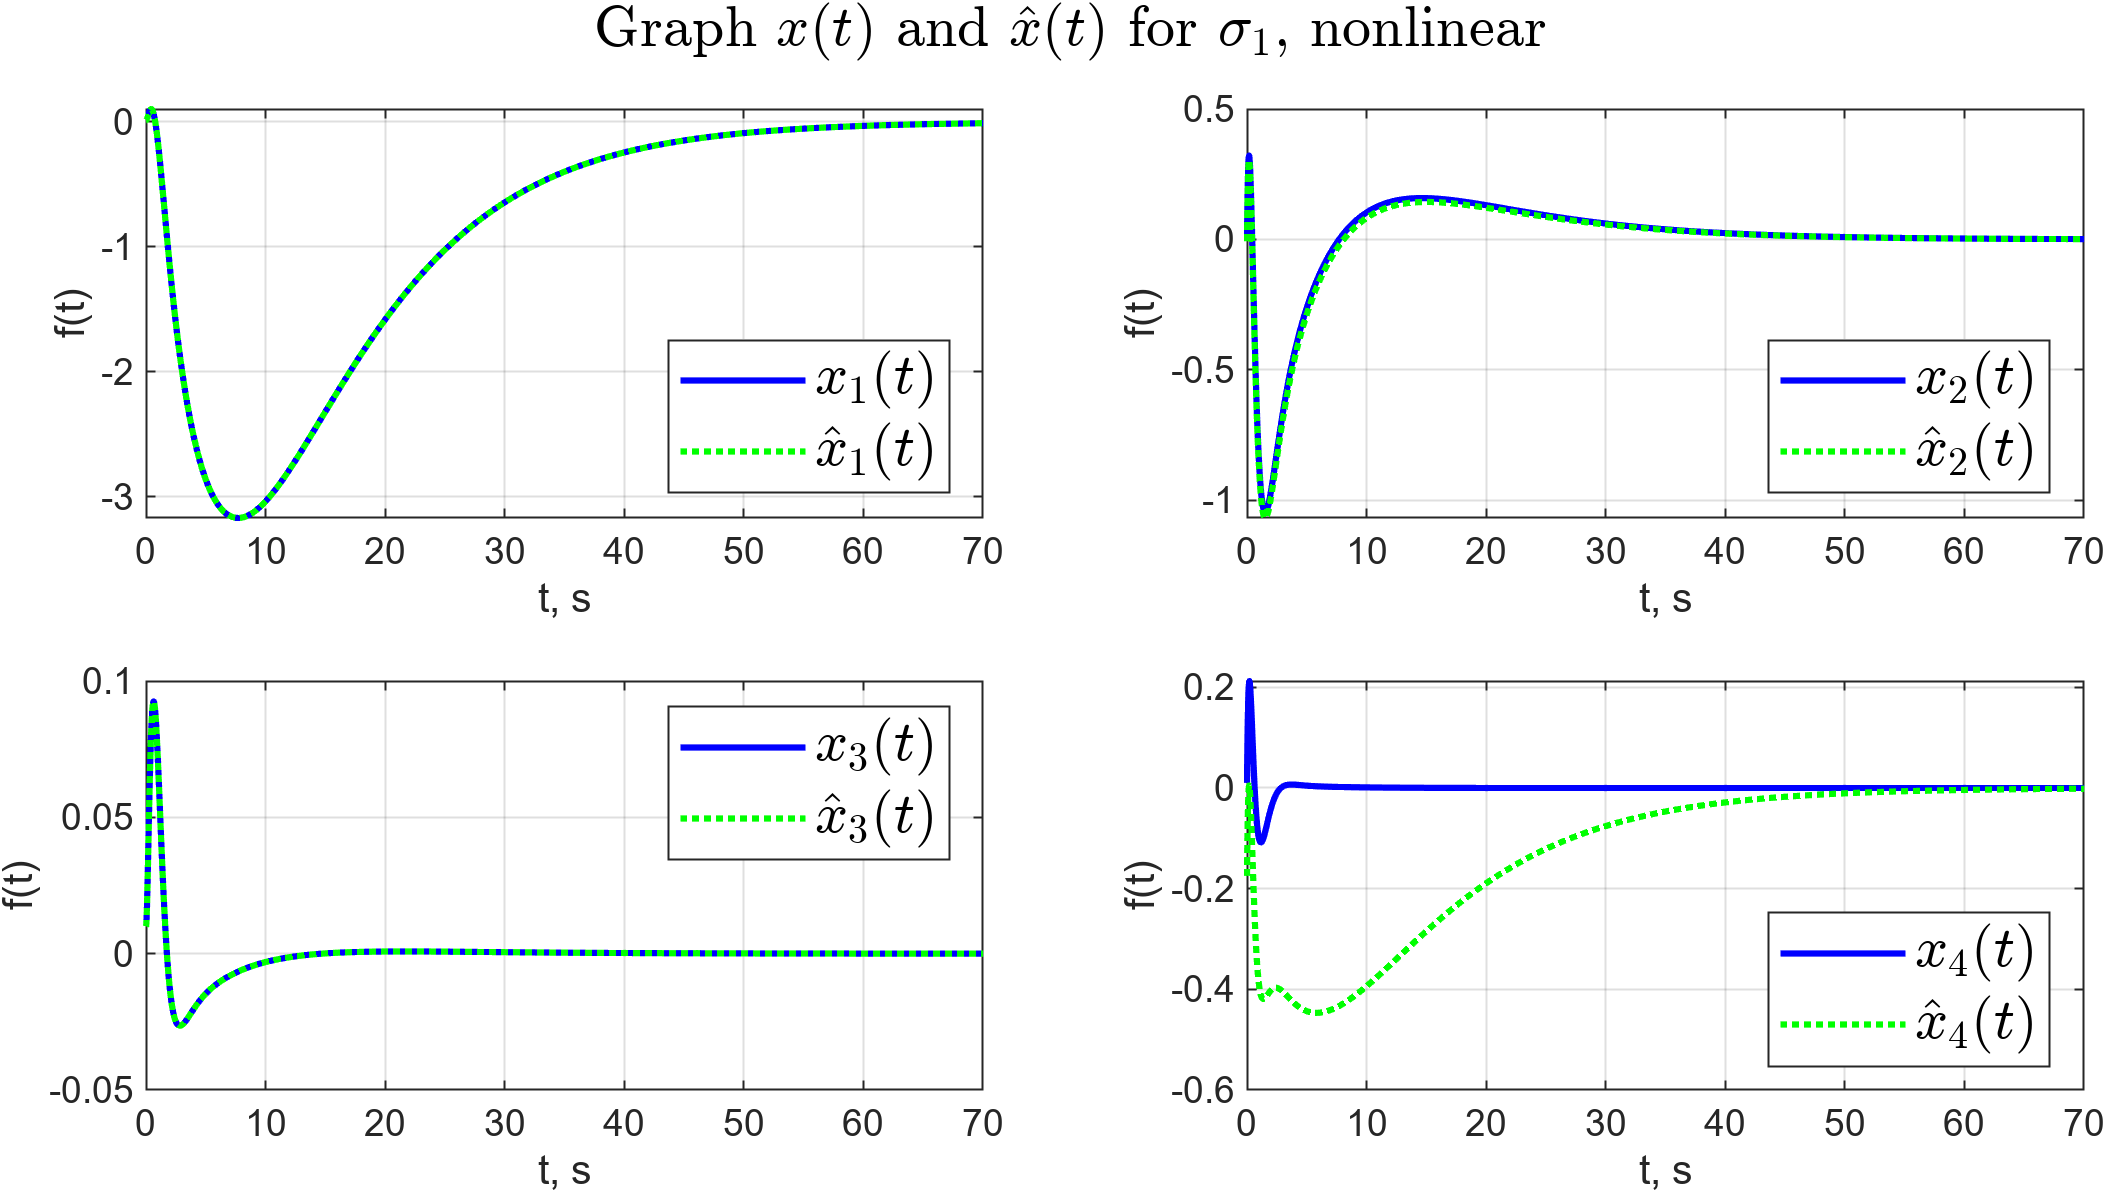
\includegraphics[width=1\linewidth]{pic/3_xx_nlin_02_LW2.png}}
\caption{Графики $x(t)$ и $\hat{x}(t)$ для $ \sigma_1 (\Gamma) = \{ -0.1, -0.2 \}$.}
\label{3_xx_nlin_02_LW2}
\end{figure}

\begin{figure}[!h]
\center{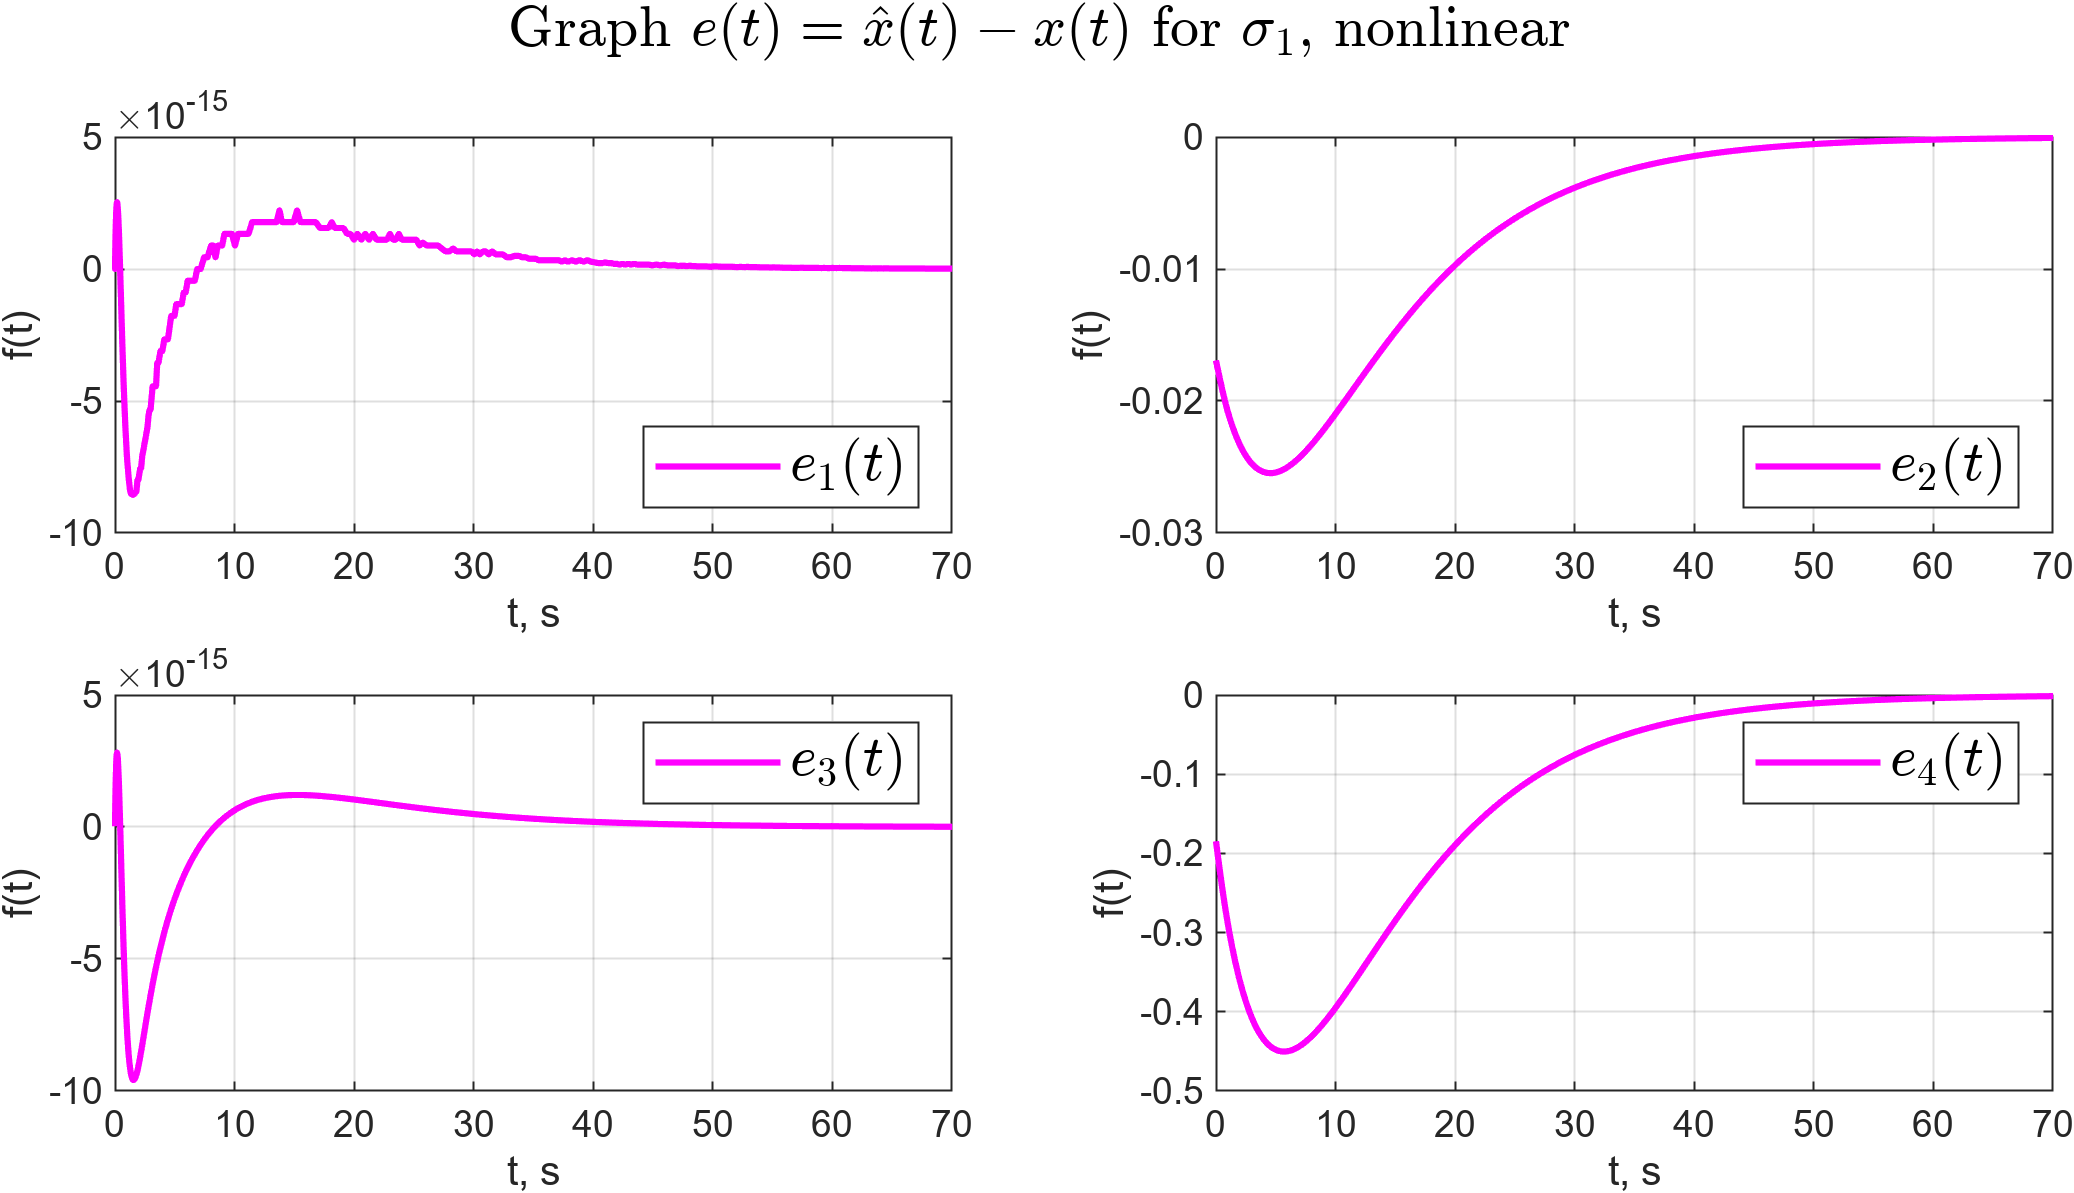
\includegraphics[width=1\linewidth]{pic/3_e_nlin_02_LW2.png}}
\caption{Графики $e (t) =\hat{x}(t) - x(t)$ для $ \sigma_1 (\Gamma) = \{ -0.1, -0.2 \}$.}
\label{3_e_nlin_02_LW2}
\end{figure}


\begin{figure}[!h]
\center{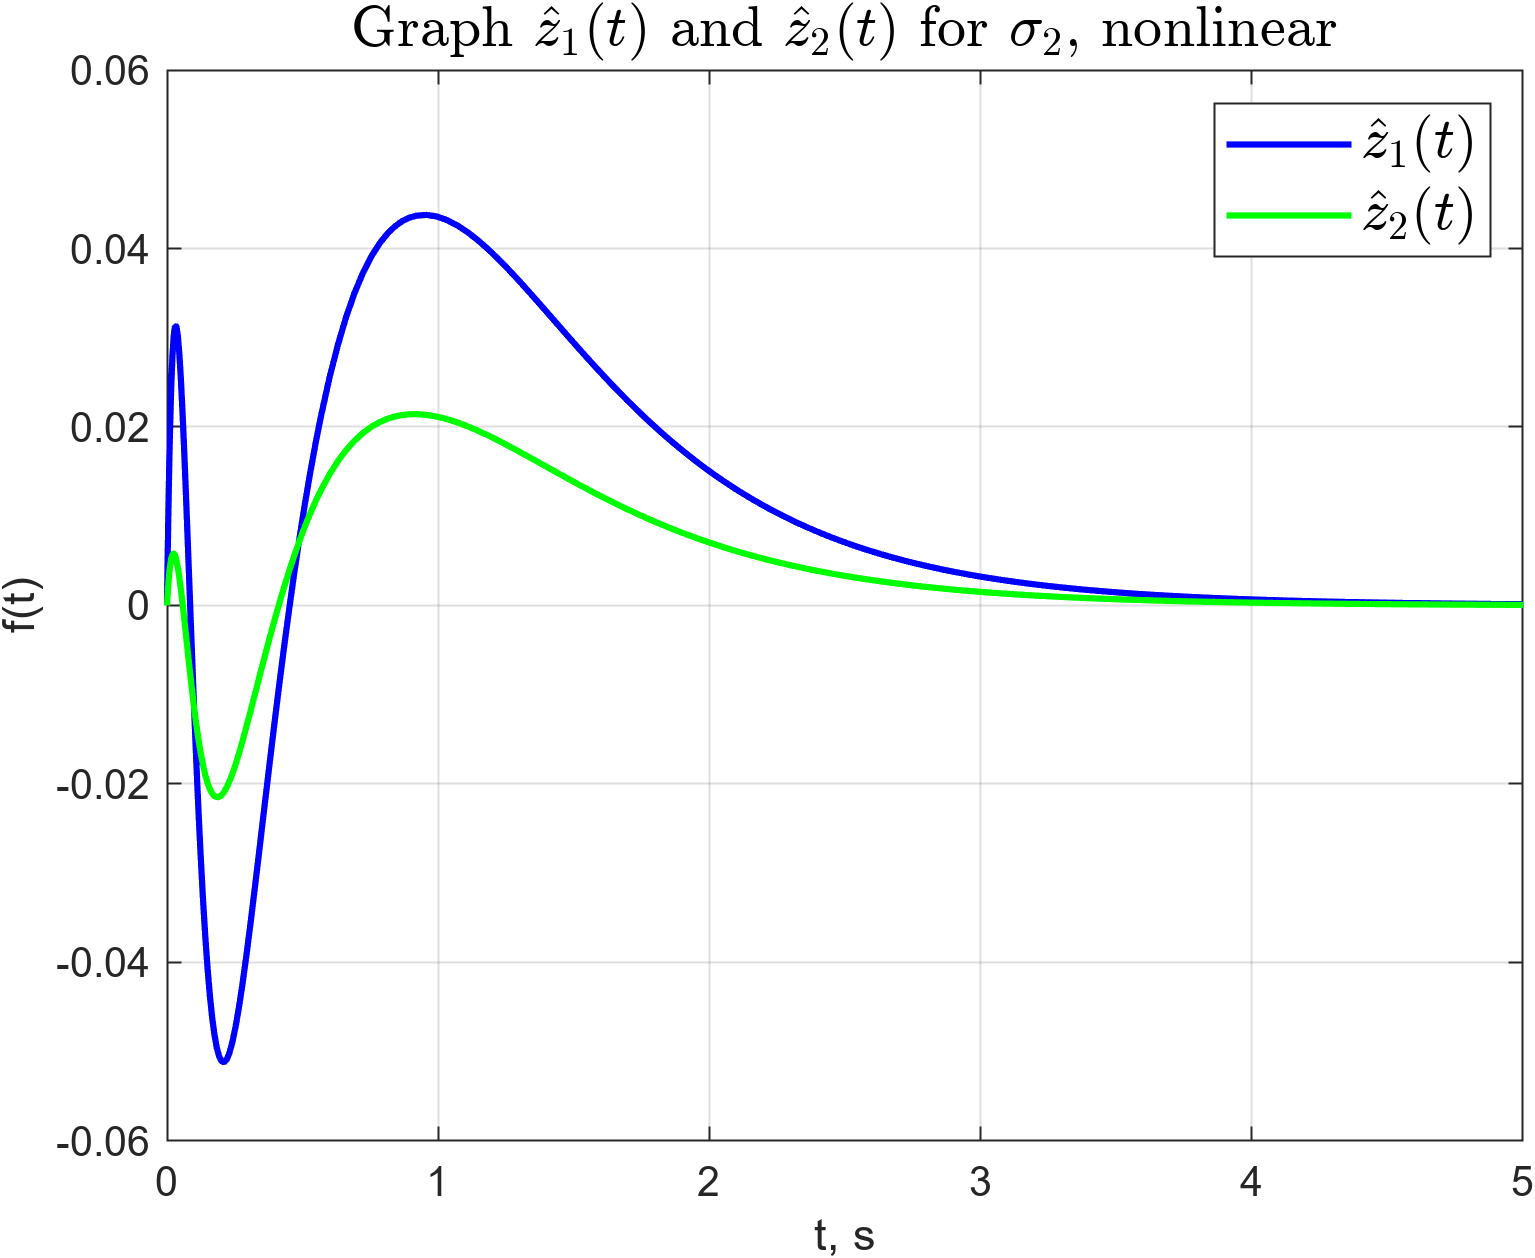
\includegraphics[width=0.6\linewidth]{pic/3_z_nlin_02_LW3.png}}
\caption{График $\hat{z}(t)$ для $ \sigma_2 (\Gamma) = \{ -10, -20 \}$.}
\label{3_z_nlin_02_LW3}
\end{figure}

\begin{figure}[!h]
\center{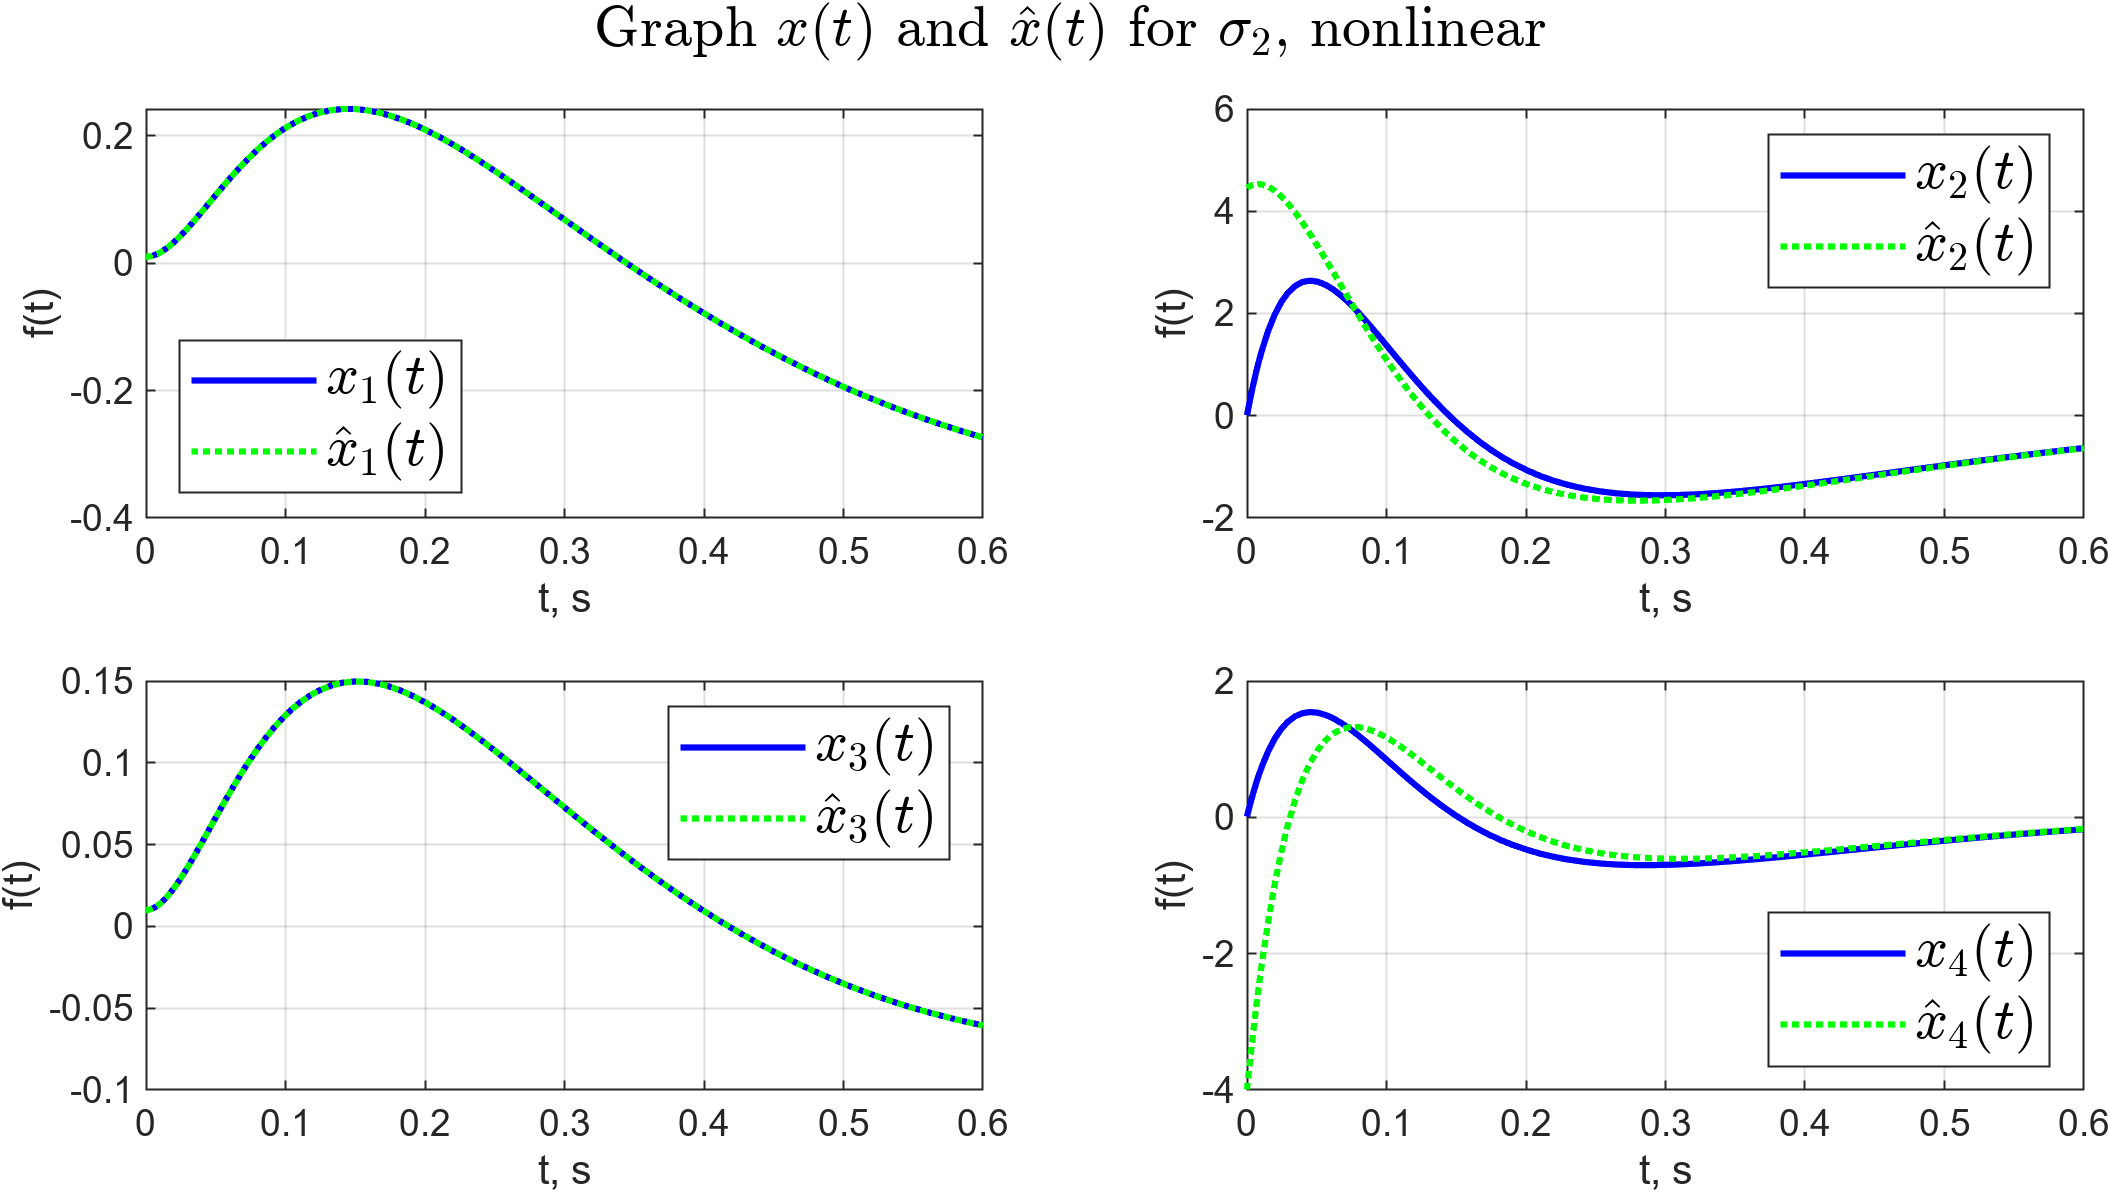
\includegraphics[width=1\linewidth]{pic/3_xx_nlin_02_LW3.png}}
\caption{Графики $x(t)$ и $\hat{x}(t)$ для $ \sigma_2 (\Gamma) = \{ -10, -20 \}$.}
\label{3_xx_nlin_02_LW3}
\end{figure}

\begin{figure}[!h]
\center{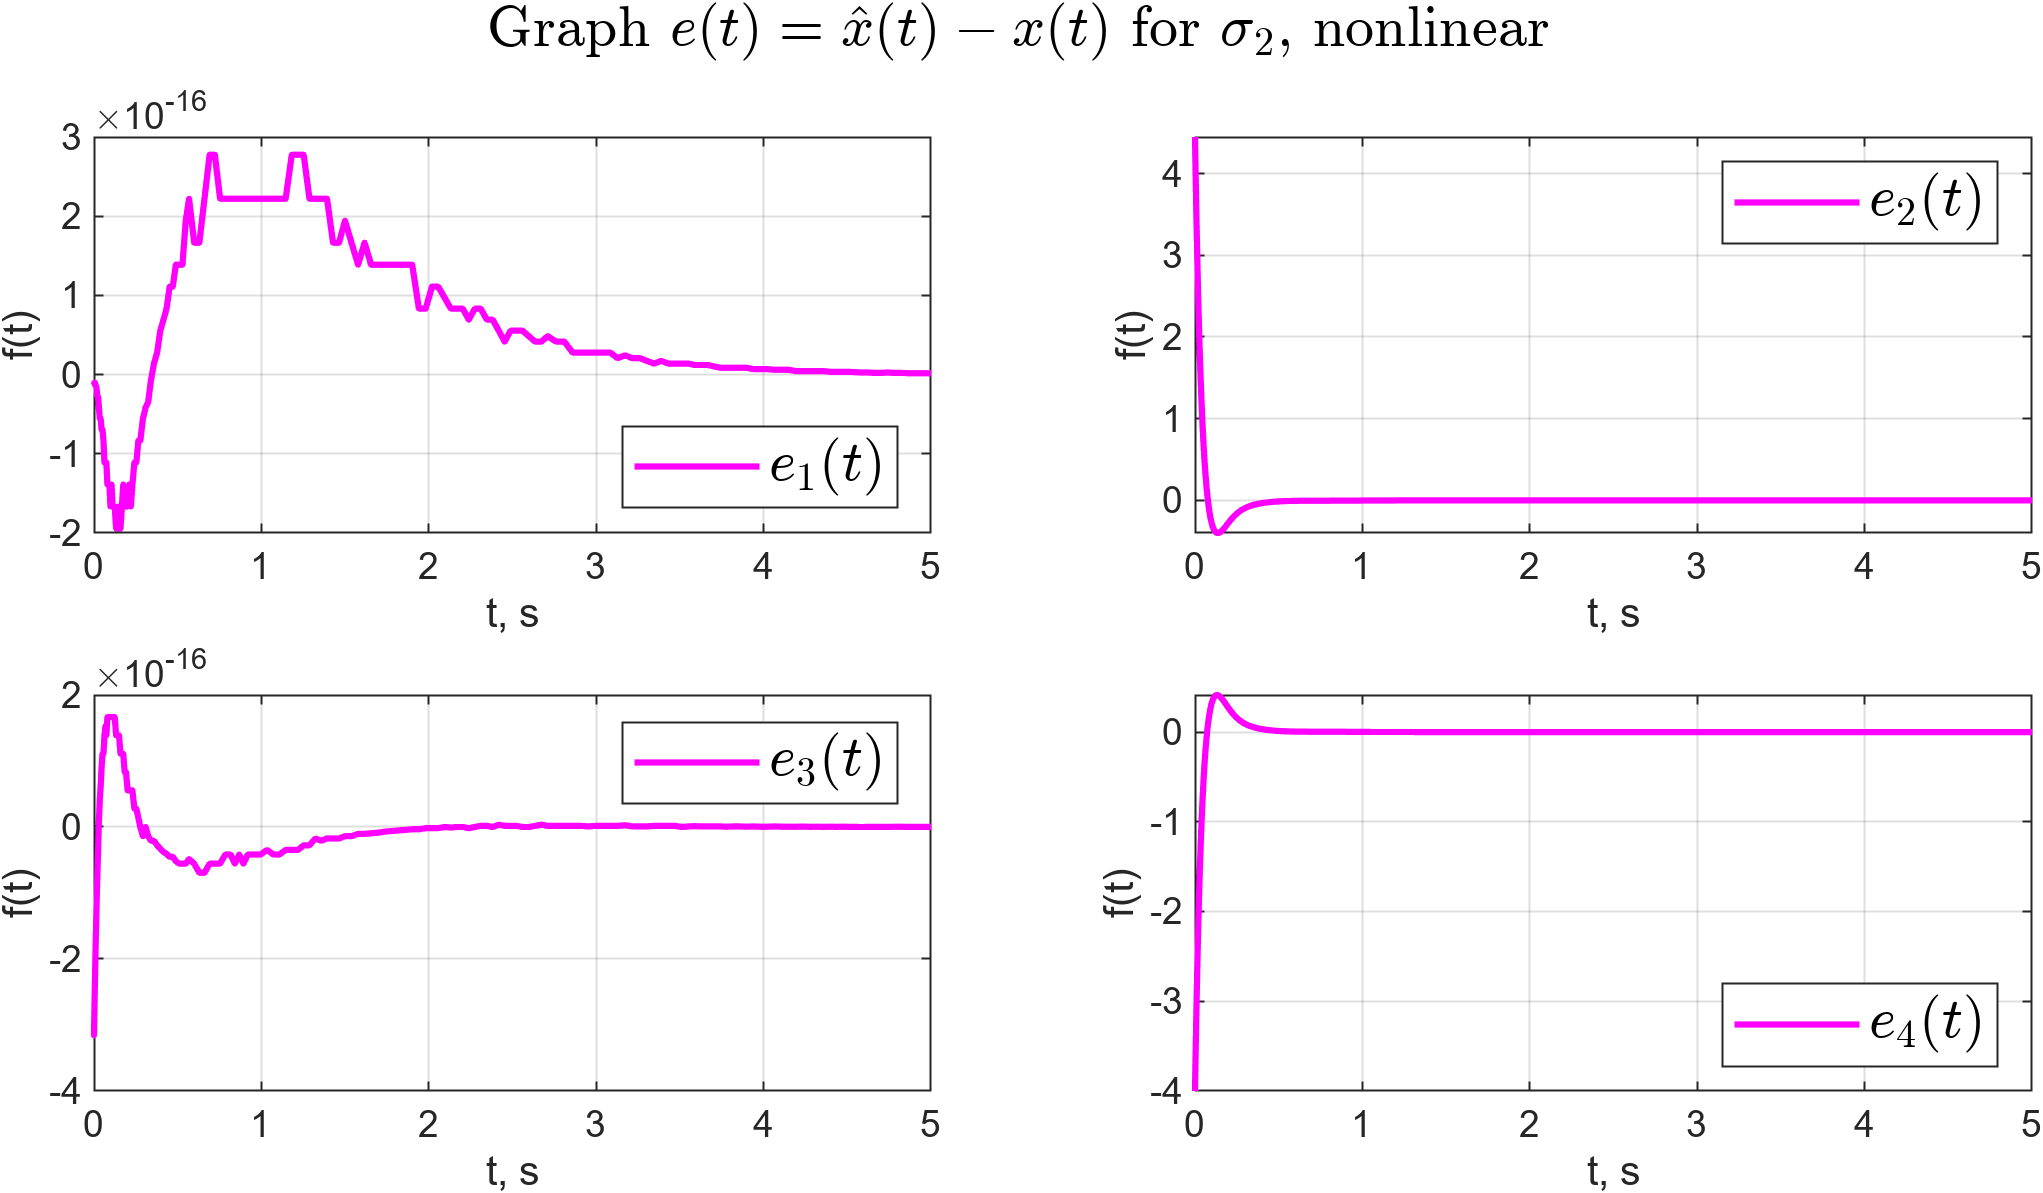
\includegraphics[width=1\linewidth]{pic/3_e_nlin_02_LW3.png}}
\caption{Графики $e (t) =\hat{x}(t) - x(t)$ для $ \sigma_2 (\Gamma) = \{ -10, -20 \}$.}
\label{3_e_nlin_02_LW3}
\end{figure}


\begin{figure}[!h]
\center{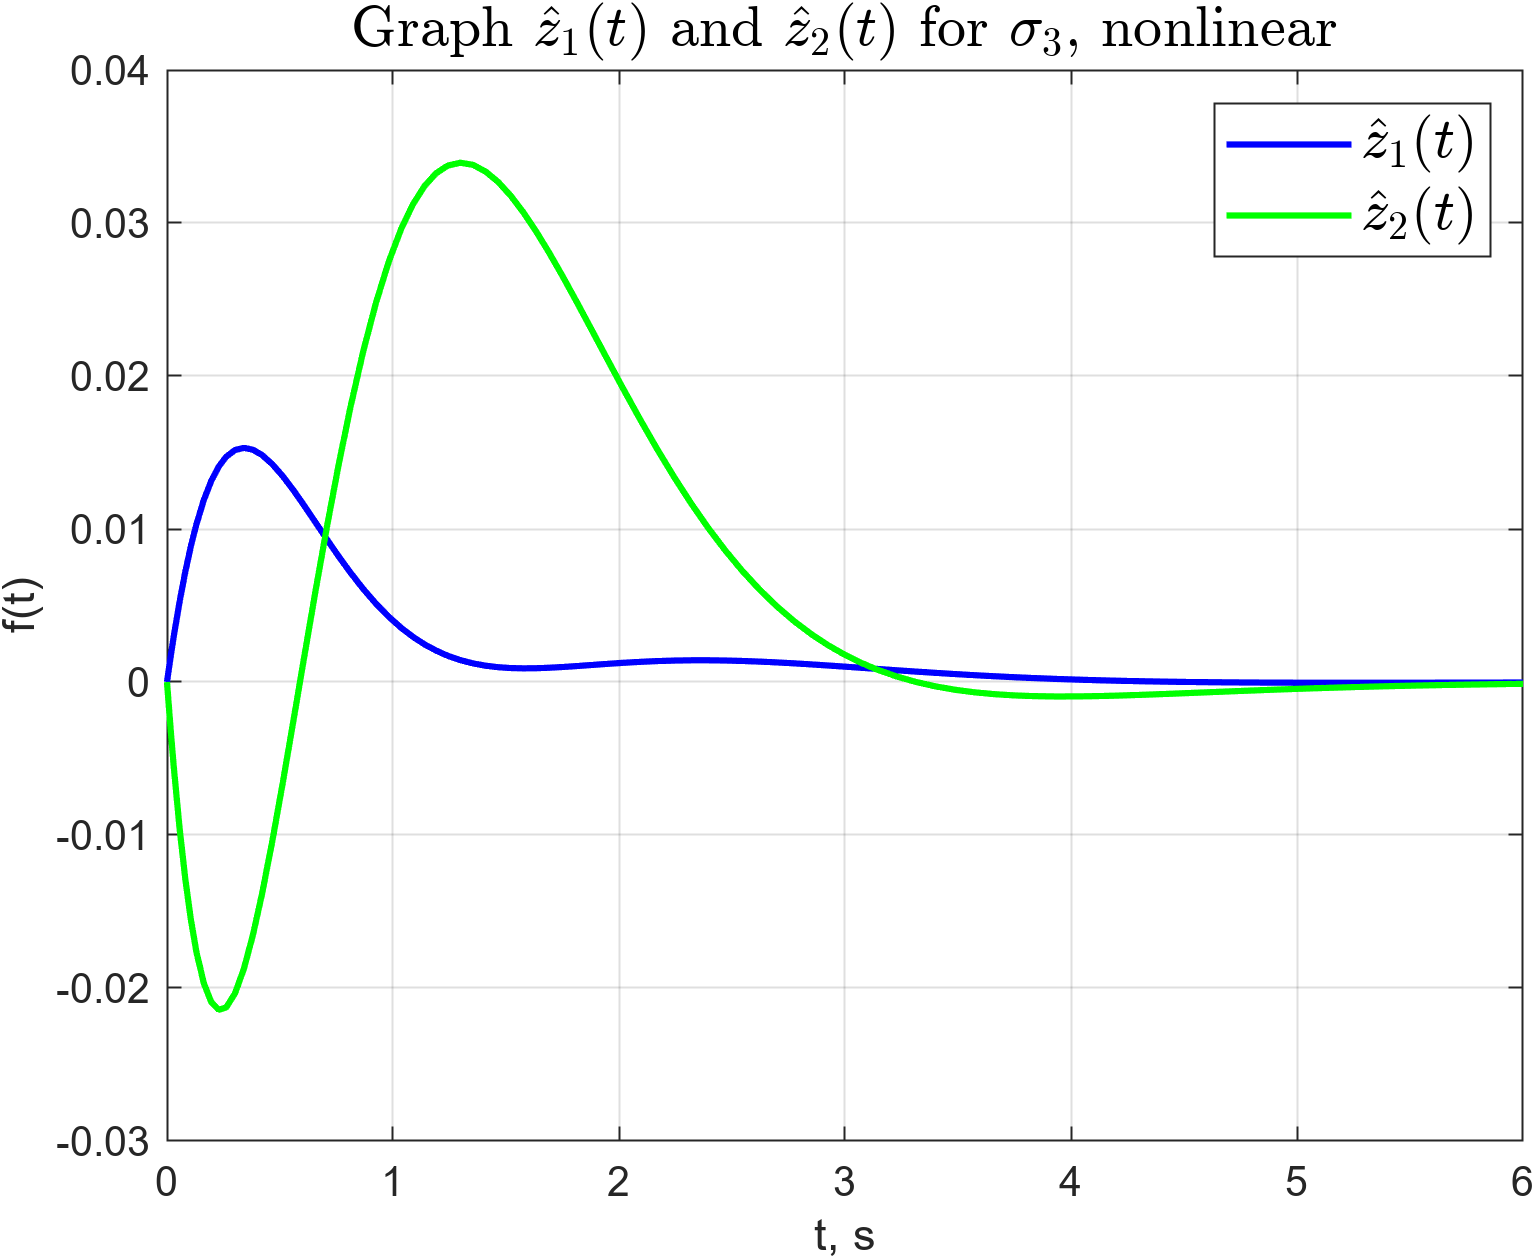
\includegraphics[width=0.6\linewidth]{pic/3_z_nlin_02_LW4.png}}
\caption{График $\hat{z}(t)$ для $ \sigma_3 (\Gamma) = \{ -2 \pm i \}$.}
\label{3_z_nlin_02_LW4}
\end{figure}

\begin{figure}[!h]
\center{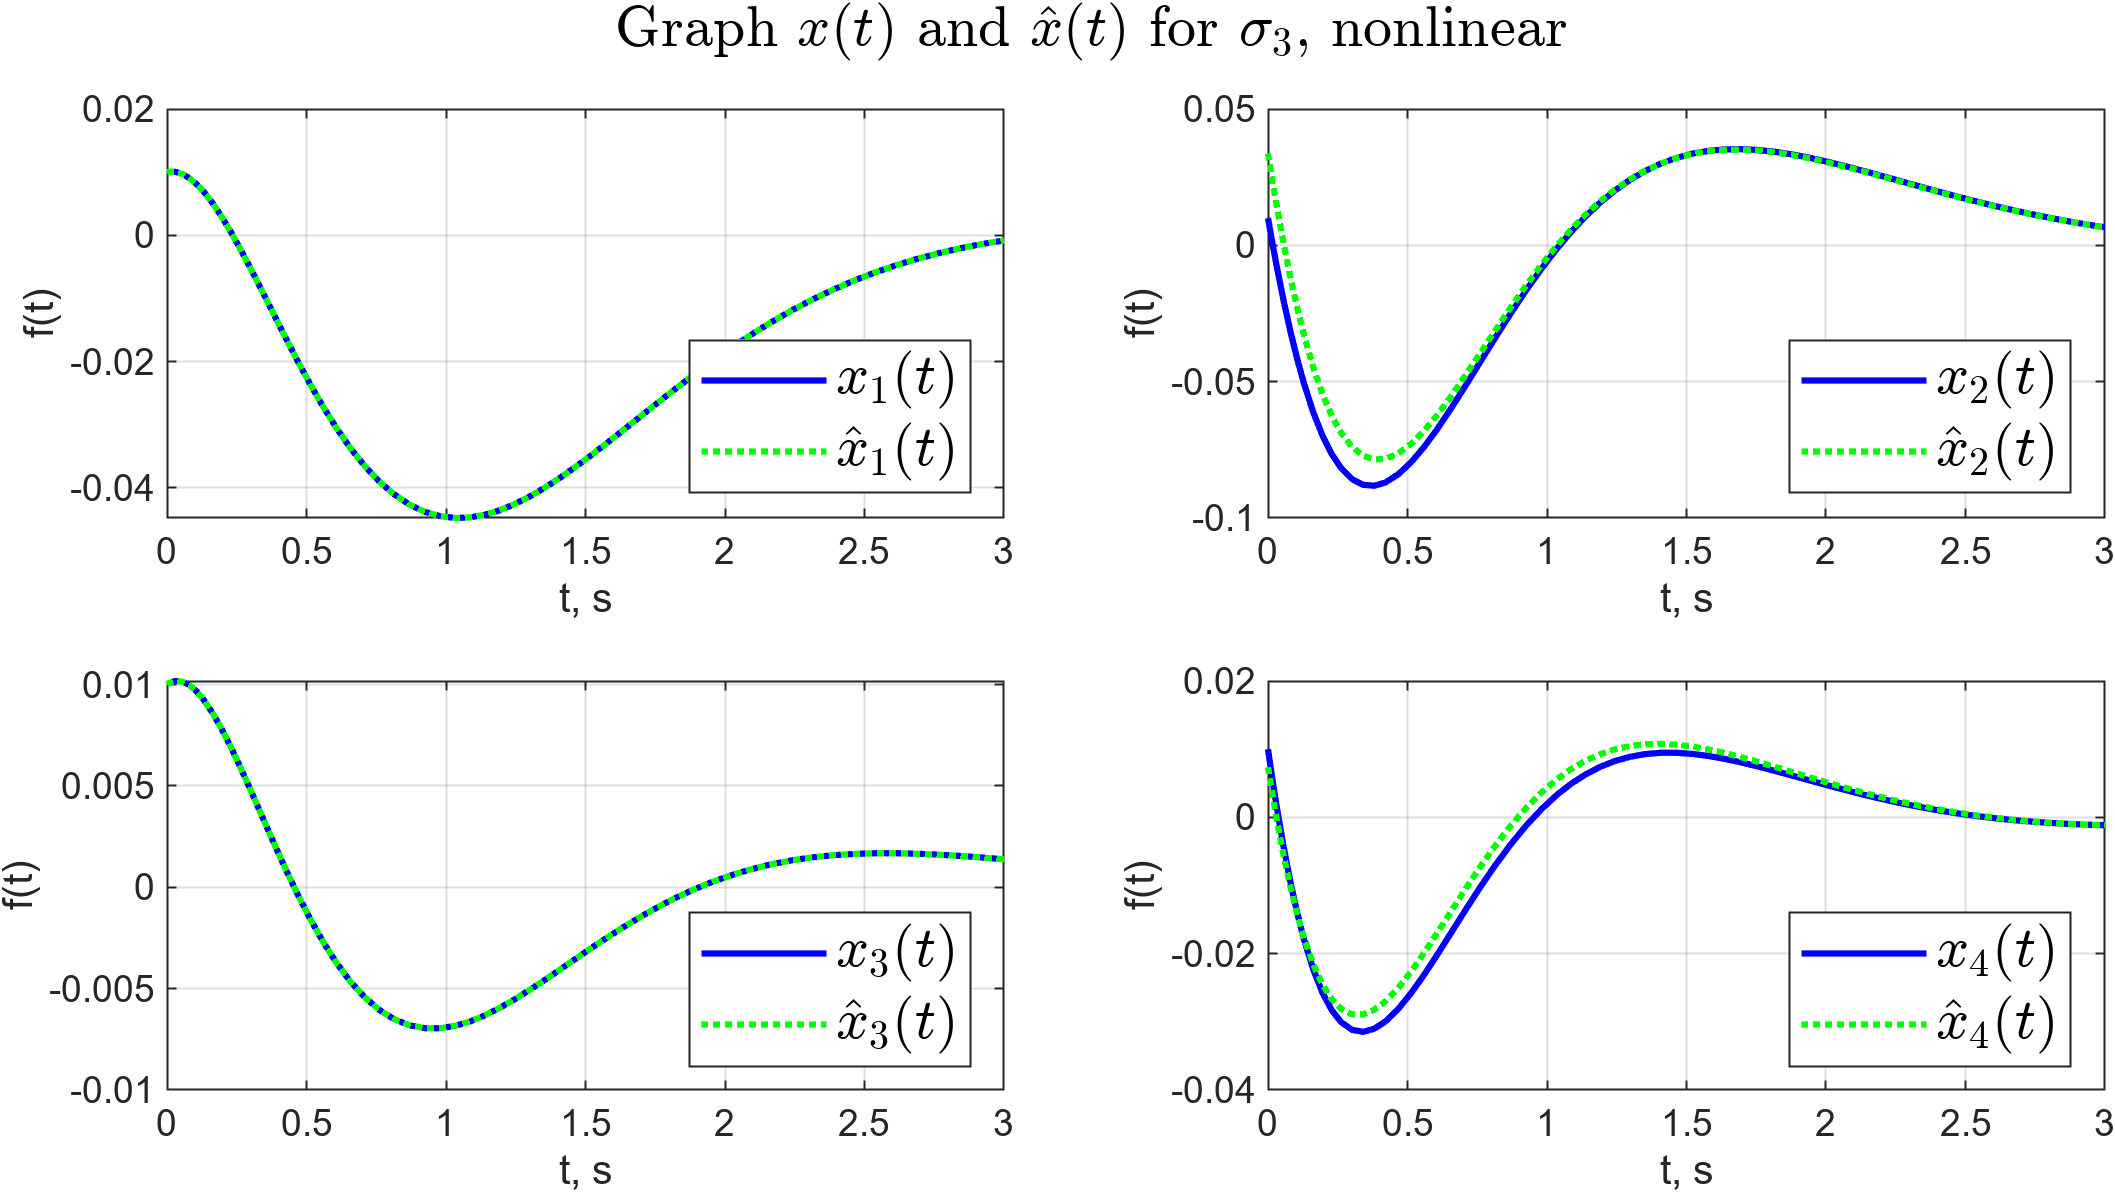
\includegraphics[width=1\linewidth]{pic/3_xx_nlin_02_LW4.png}}
\caption{Графики $x(t)$ и $\hat{x}(t)$ для $ \sigma_3 (\Gamma) = \{ -2 \pm i \}$.}
\label{3_xx_nlin_02_LW4}
\end{figure}

\begin{figure}[!h]
\center{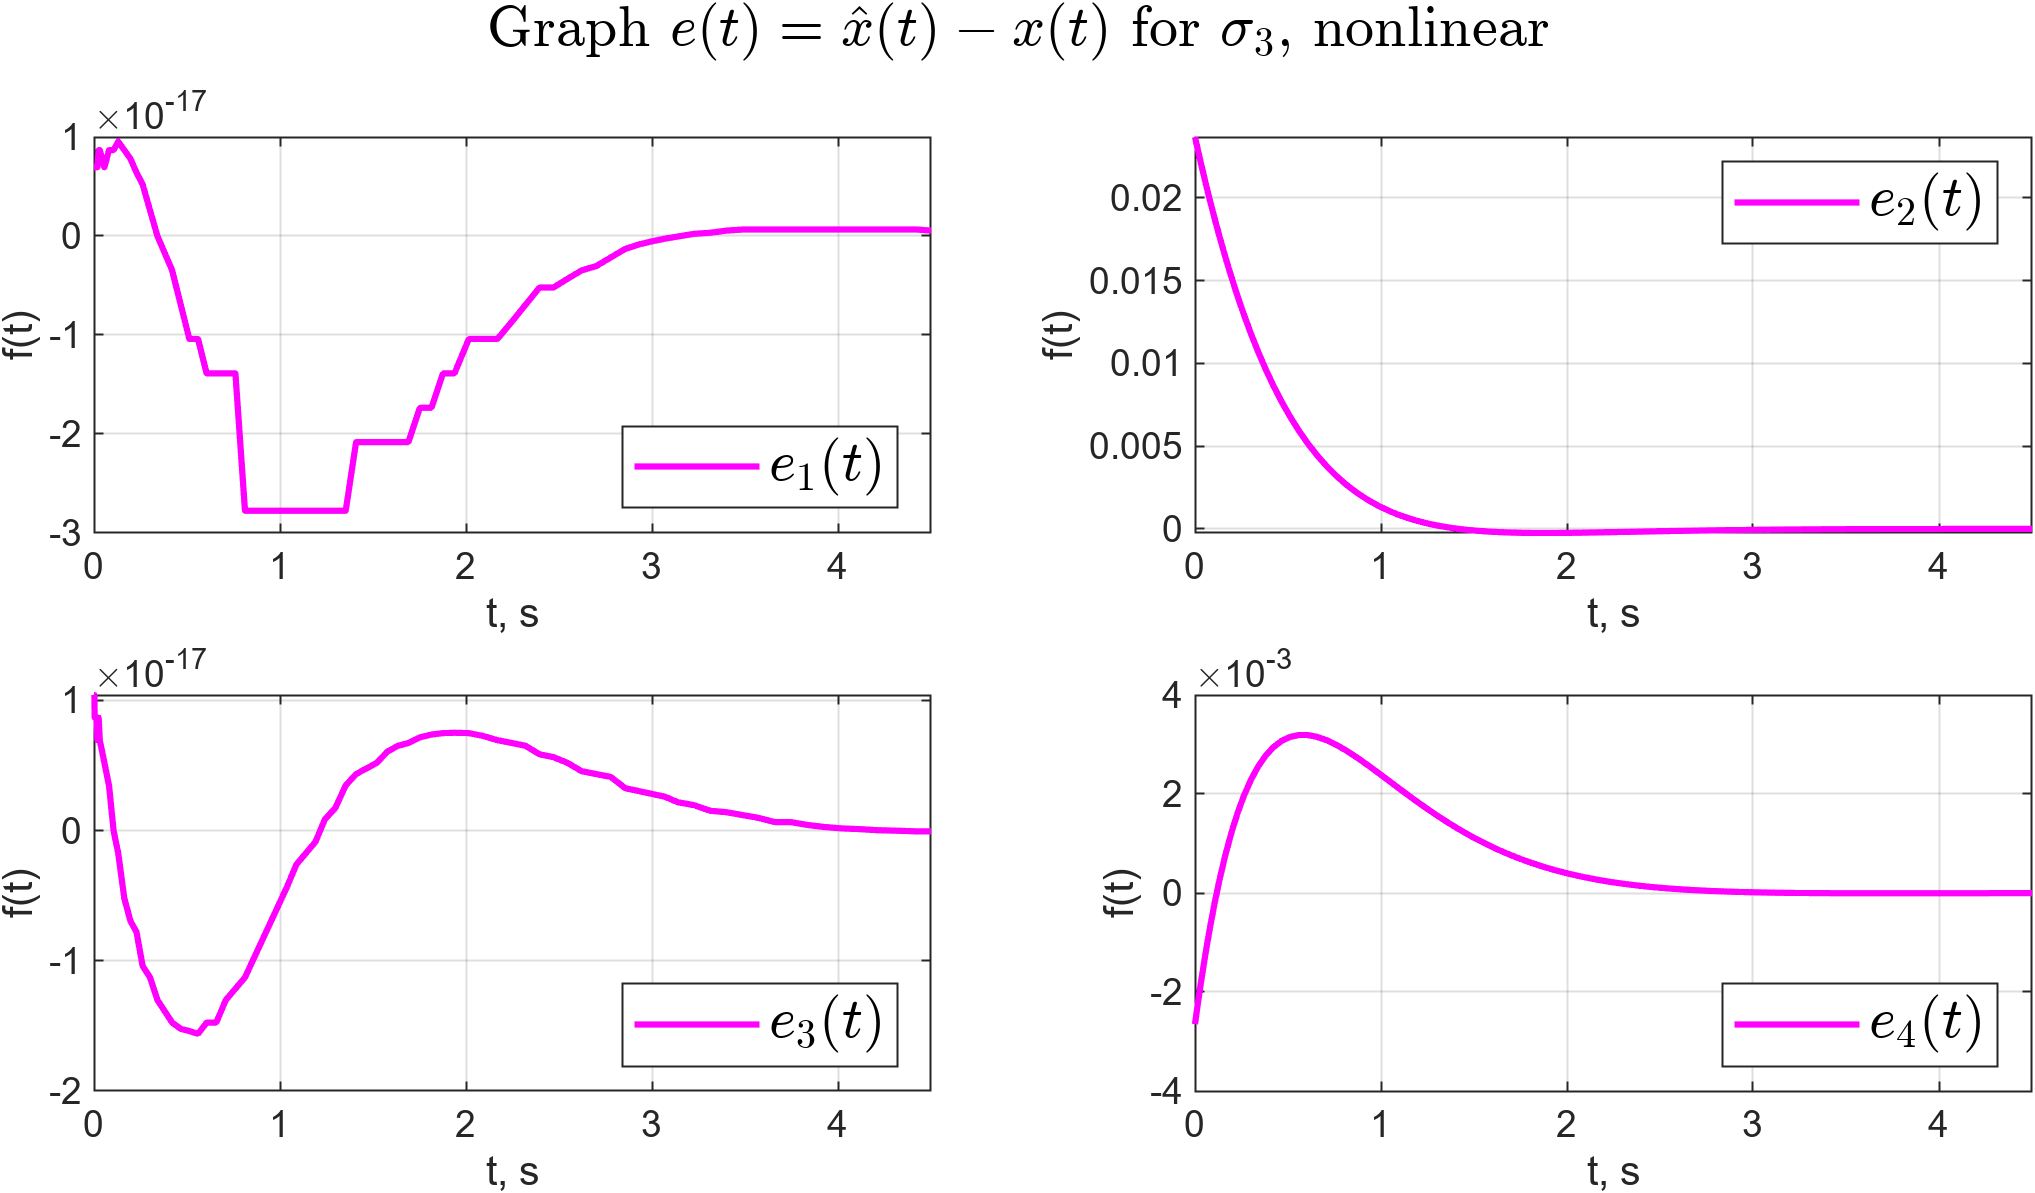
\includegraphics[width=1\linewidth]{pic/3_e_nlin_02_LW4.png}}
\caption{Графики $e (t) =\hat{x}(t) - x(t)$ для $ \sigma_3 (\Gamma) = \{ -2 \pm i \}$.}
\label{3_e_nlin_02_LW4}
\end{figure}





\newpage
\,
\newpage
\,
\newpage
\,
\newpage
Как и в случае наблюдателя полной размерности, для наблюдателя пониженной размерности также время, за которое ошибка наблюдателя становится неотличима от нуля, возрастает при уменьшении собственных значений для наблюдателя (рисунок \ref{3_e_nlin_02_LW2}) и уменьшается, при увеличении собственных чисел (рисунок \ref{3_e_nlin_02_LW3}).

\subsection{Сравнение работы наблюдателей полной и пониженной размерности}

В ходе исследования для наблюдателя пониженной размерности были подобраны спектры близкие к соответствующим наборам собственных чисел для наблюдателя полной размерности. 

Время, за которое ошибка наблюдателя становится неотличима от нуля, сопоставимо для наблюдателей полной и пониженной размерности для близких спектров. 

Для наблюдателя пониженной размерности практически нулевая ошибка для $x_1$ и $x_3$, так как эти компоненты напрямую попадают в вывод $y_1$ и $y_2$ соответственно, то есть они измеримы. Наблюдатель полного порядка в данном случае избыточен и накапливает большую ошибку. 


\section{Синтез регулятора по выходу}
Построим регулятор, стабилизирующий маятник и тележку в условиях, когда измерению доступны только сигналы $y_1$ и $y_2$, то есть положение тележки $a(t)$ и угол отклонения маятника от вертикали $\varphi(t)$. Для этого будем использовать наблюдатель пониженной размерности из предыдущего пункта и основанный на нем закон управления $u = K \hat{x}$.


Постараемся подобрать такие спектры наблюдателя и регулятора, при которых переходные процессы в замкнутой системе будут иметь малое время переходного процесса, малое перерегулирование и малую величину управляющего воздействия. Поэтому для каждого набора спектров наблюдателя и регулятора будем находить  максимальные значения модуля координаты тележки $a(t)$, угла отклонения маятника от вертикали $\varphi(t)$ и управляющего воздействия $u(t)$, а также фиксировать время переходного процесса (как последний момент времени, когда координата тележки или угол отклонения маятника отличался от нуля более, чем на 0.0001).

\begin{table}[h]
\centering
\caption{Результаты моделирования для различных наборов спектров}
\label{3_tab_2}
\begin{tabular}{ccccccc}
\toprule
$\sigma_{reg}$  & $\sigma_{obs}$  & $\max |\varphi|$ & $\max |a|$ & $\max |u|$& t, s \\
\midrule
$\{ -1, -1, -1, -1\}$  & $\{-1, -1.5 \}$  & 0.011  &  0.15  &  67 & 15  \\
$\{ -3, -2.5, -2, -1.5\}$  & $\{-1, -1.5 \}$  & 0.010  &  0.042  &  203 & 6.6  \\
$\{ -0.5, -0.4, -0.3, -0.2\}$  & $\{-1, -1.5 \}$  & 0.014  &  1.58  &  41 & 64 \\
$\{ -1, -1, -1, -1\}$  & $\{-5, -6 \}$  & 0.017  &  0.16  &  304 & 13  \\
$\{ -3, -2.5, -2, -1.5\}$  & $\{-5, -6 \}$  & 0.025  &  0.095  &  1493 & 6.2  \\
$\{ -0.5, -0.4, -0.3, -0.2\}$  & $\{-5, -6 \}$  & 0.016  &  1.3  &  68 & 63  \\
\bottomrule
\end{tabular}
\end{table}

Из всех представленных вариантов в таблице \ref{3_tab_2} наиболее оптимальным является набор $\sigma_{reg} = \{ -3, -2.5, -2, -1.5\}$, $\sigma_{obs}= \{-1, -1.5 \}$, графики представлены на рисунках \ref{3_x_k1l1} и \ref{3_u_k1l1}. Результаты моделирования для остальных наборов представлены на рисунках \ref{3_x_k2l1}-\ref{3_u_k3l2}.

% K2L1 -- best
\begin{figure}[!h]
\center{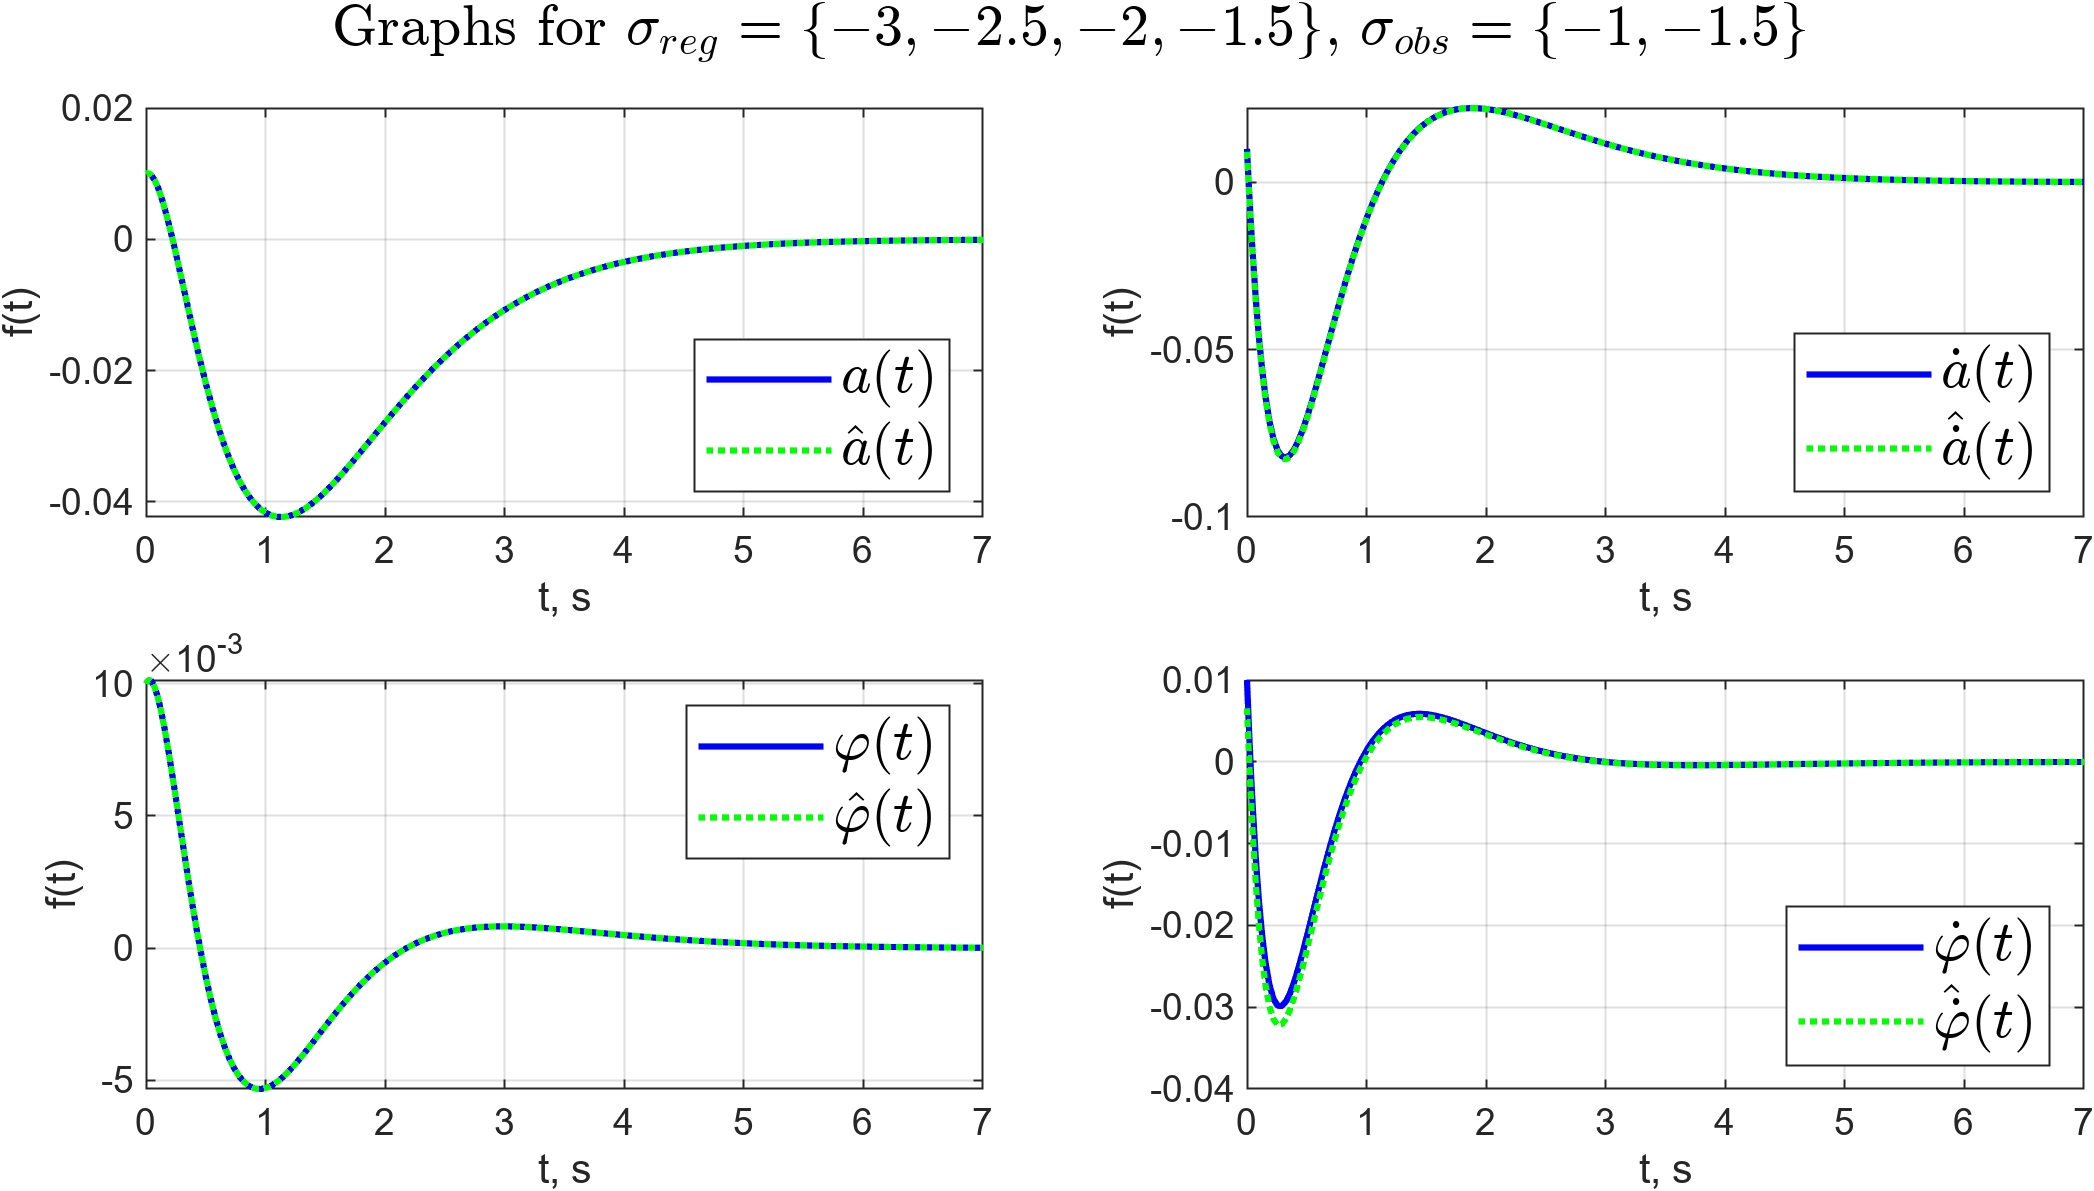
\includegraphics[width=1\linewidth]{pic_fix/3_x_k2l1.png}}
\caption{Графики векторов состояния системы и наблюдателя для $\sigma_{reg} = \{ -3, -2.5, -2, -1.5\}$, $\sigma_{obs}= \{-1, -1.5 \}$.}
\label{3_x_k1l1}
\end{figure}

\begin{figure}[!h]
	\center{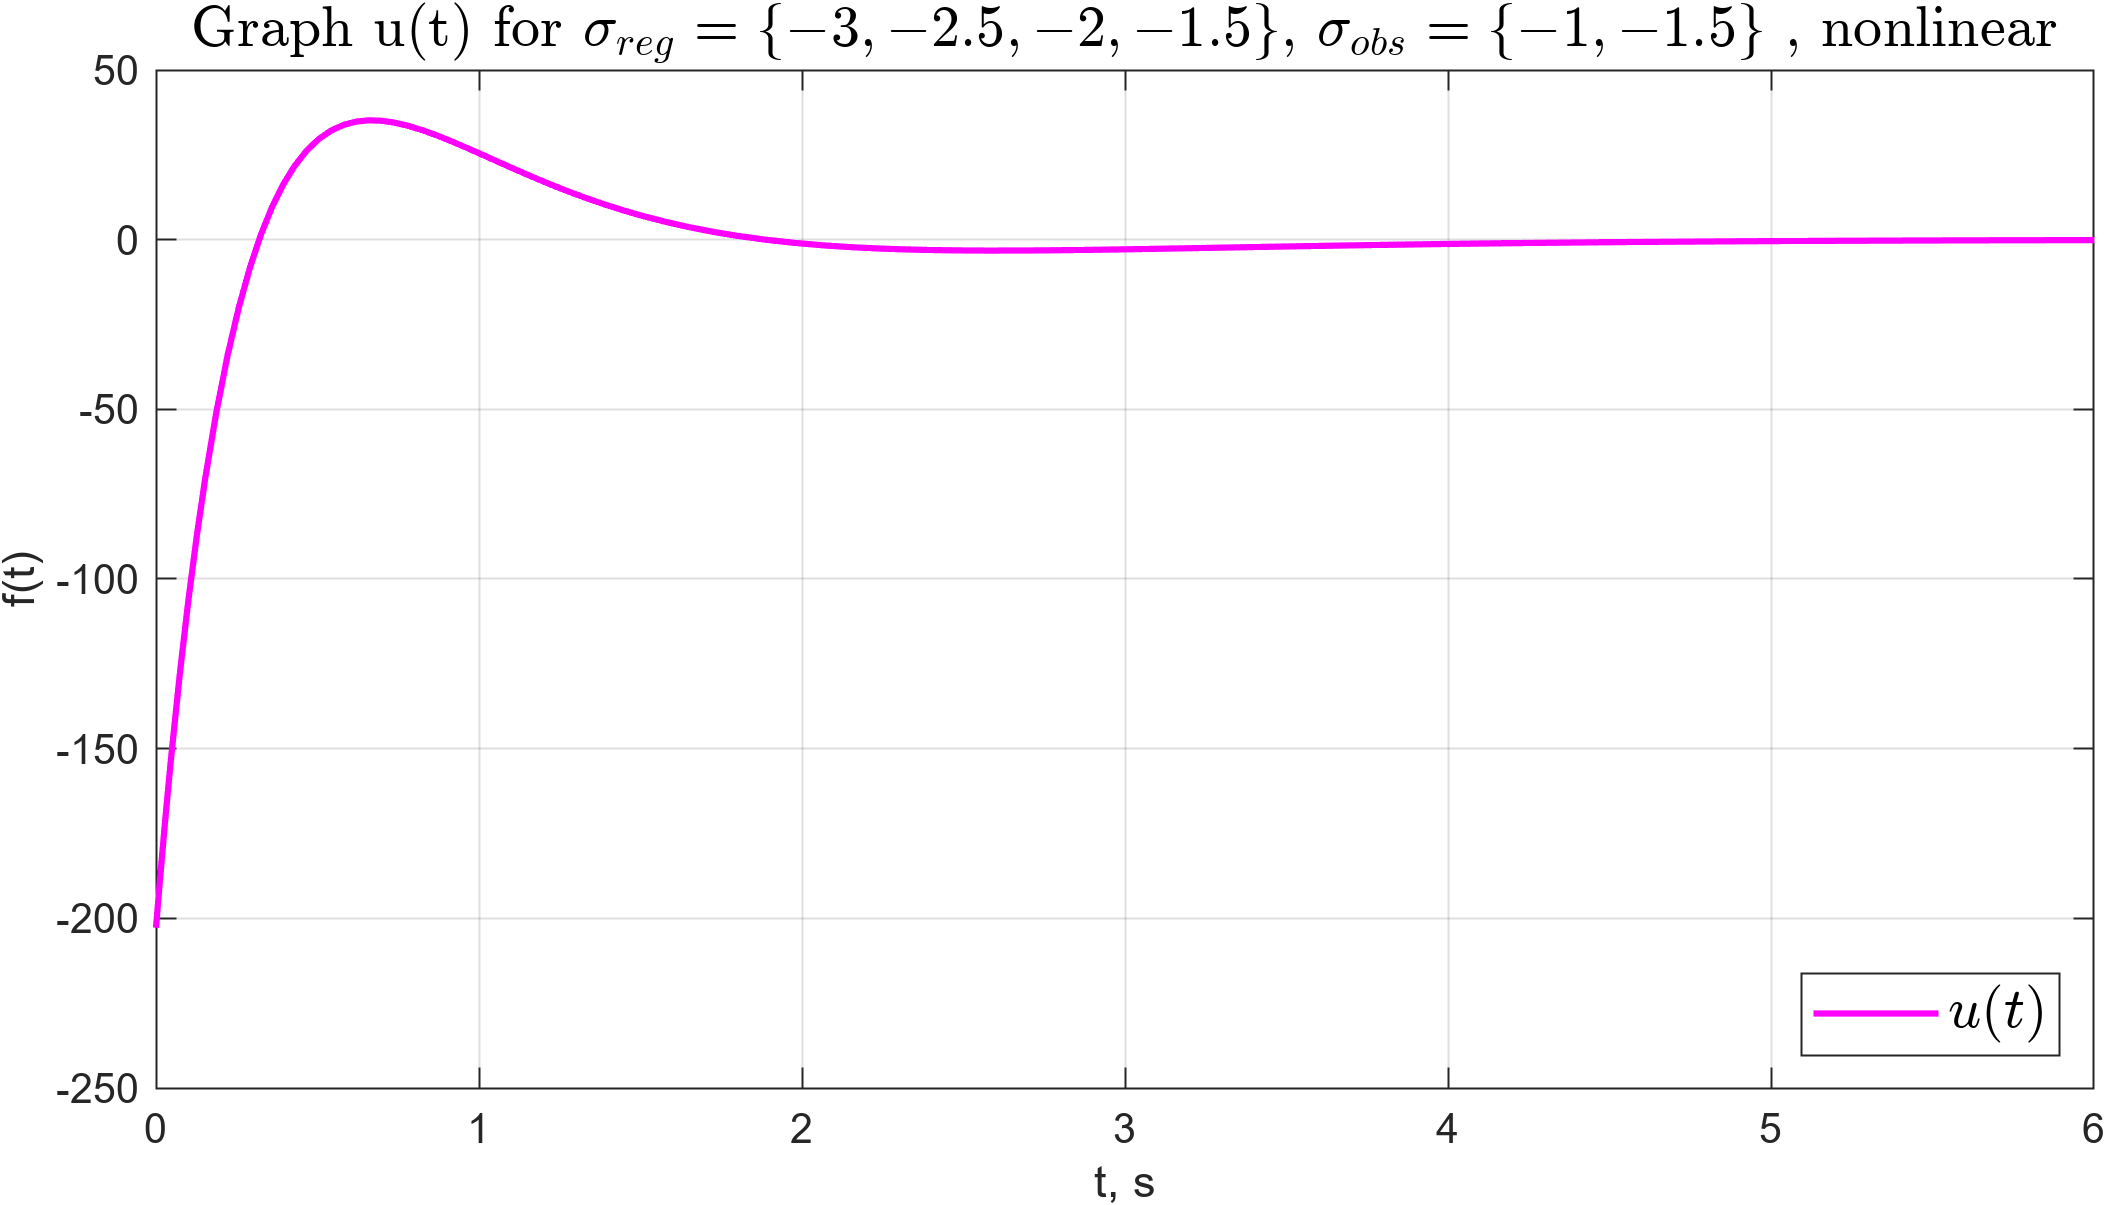
\includegraphics[width=1\linewidth]{pic_fix/3_u_k2l1.png}}
	\caption{График $u(t)$ для $\sigma_{reg} = \{ -3, -2.5, -2, -1.5\}$, $\sigma_{obs}= \{-1, -1.5 \}$.}
	\label{3_u_k1l1}
\end{figure}

% K1L1
\begin{figure}[!h]
	\center{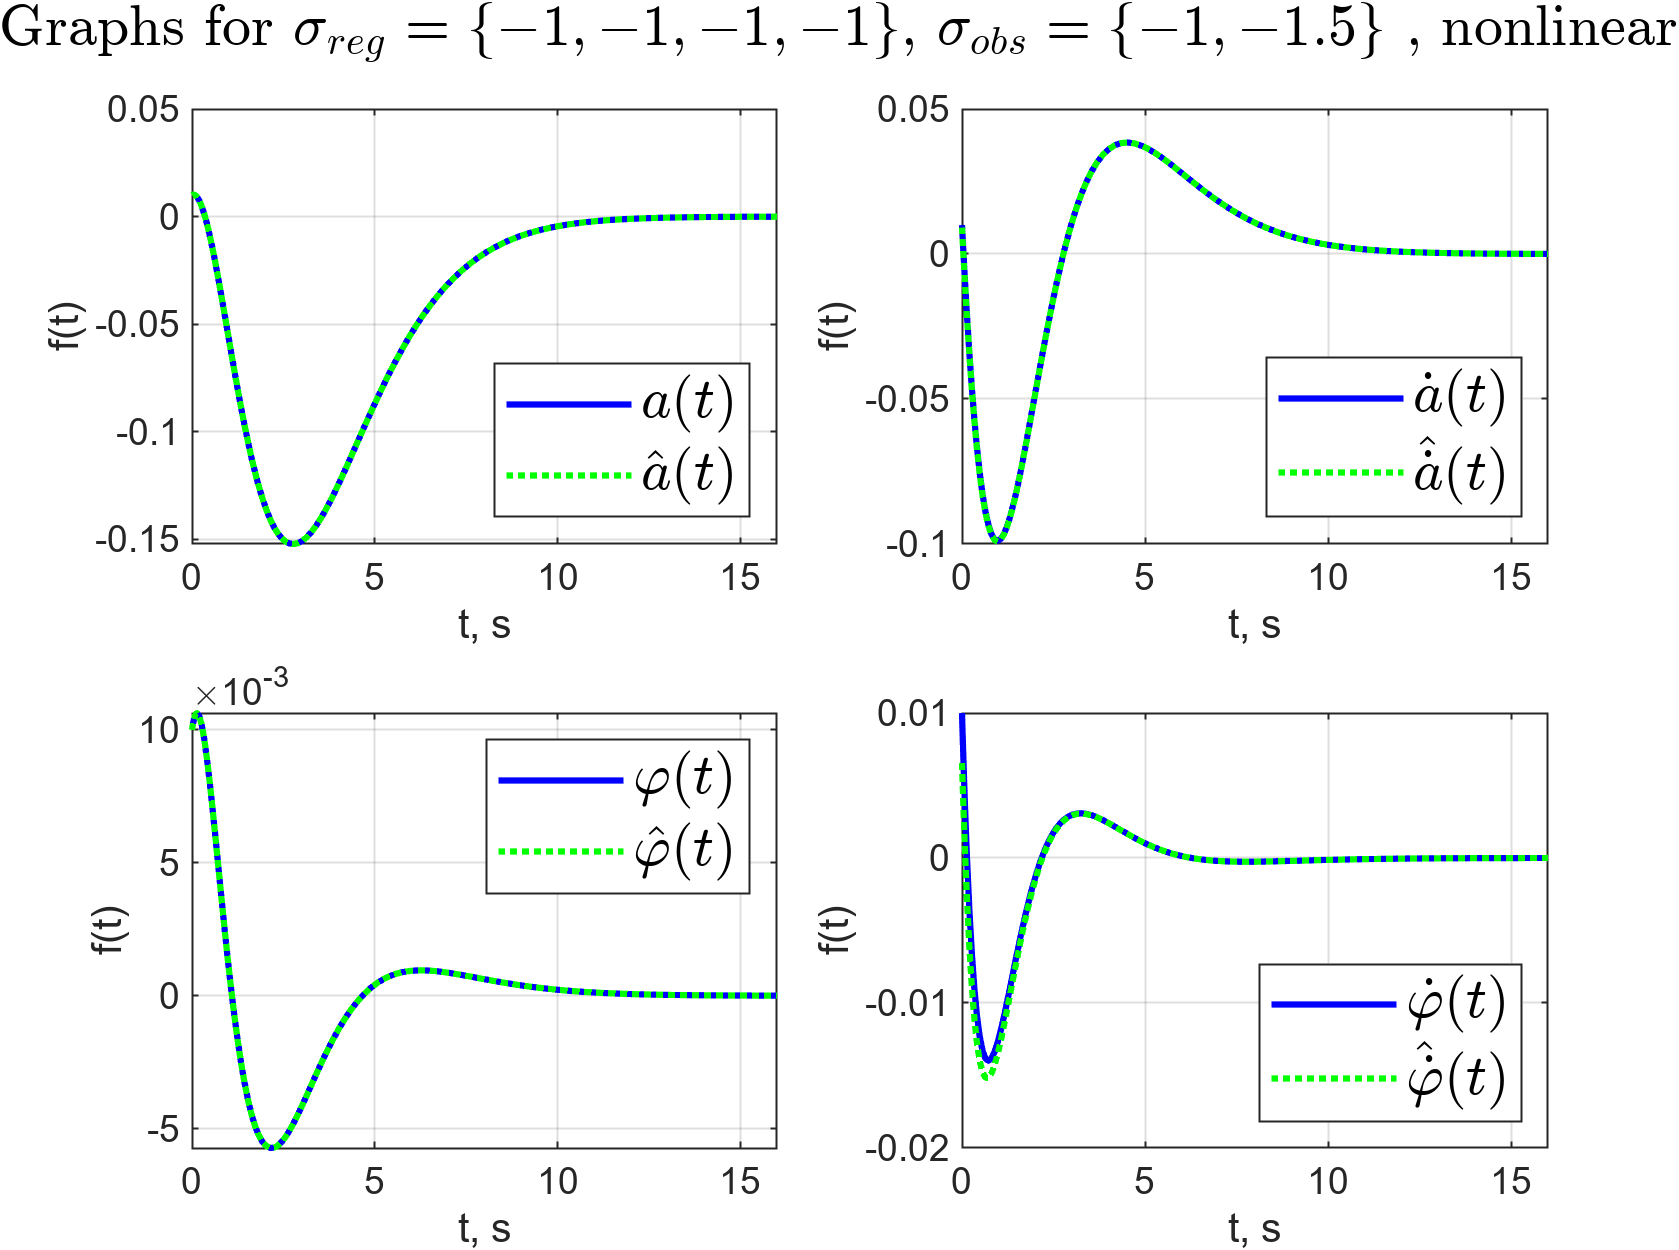
\includegraphics[width=1\linewidth]{pic/3_x_k1l1.png}}
	\caption{Графики векторов состояния системы и наблюдателя для $\sigma_{reg} = \{ -1, -1, -1, -1\}$, $\sigma_{obs}= \{-1, -1.5 \}$.}
	\label{3_x_k2l1}
\end{figure}

\begin{figure}[!h]
	\center{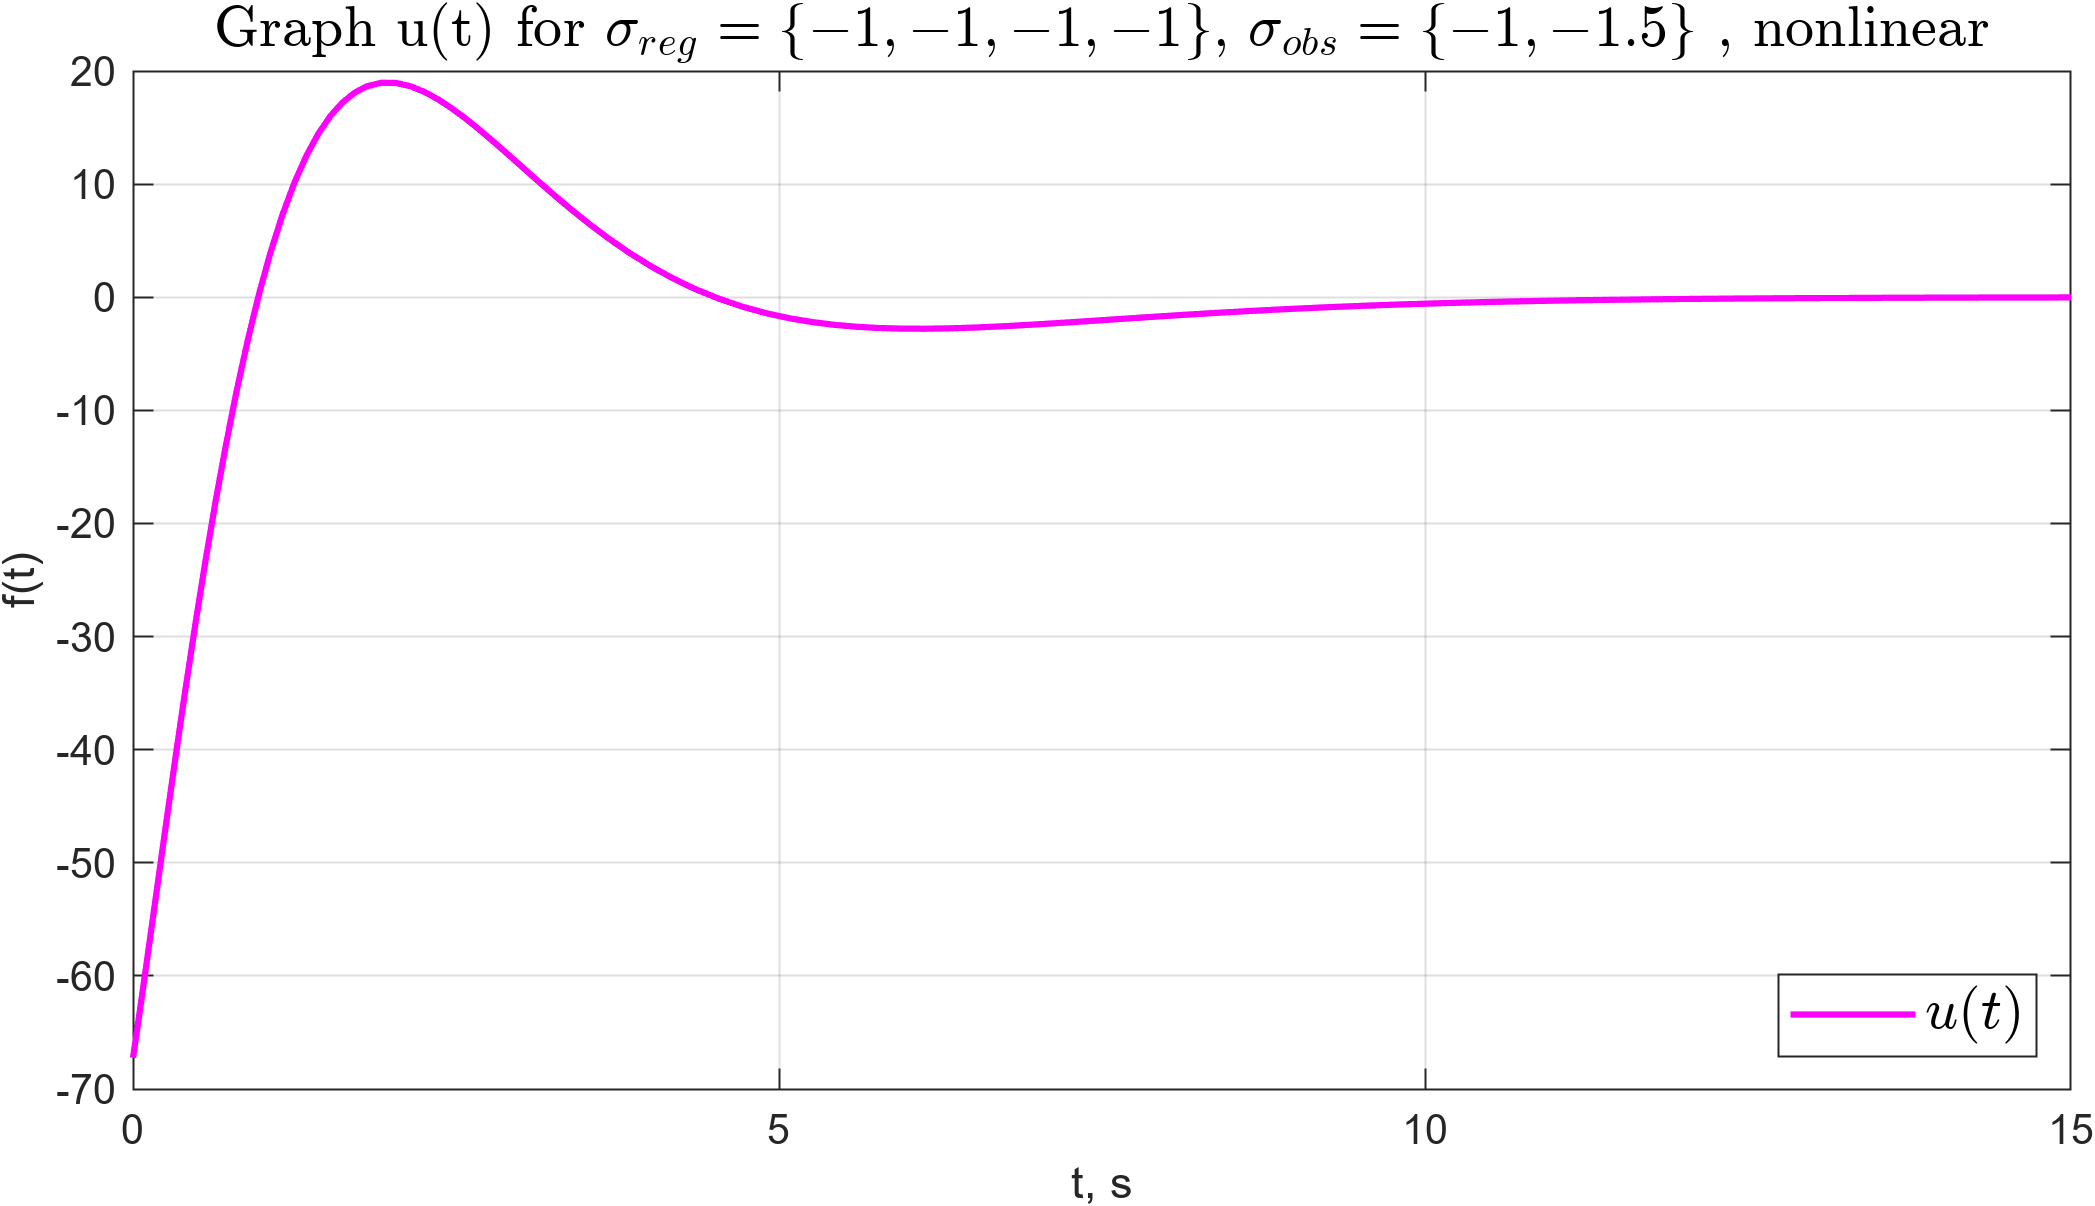
\includegraphics[width=1\linewidth]{pic/3_u_k1l1.png}}
	\caption{График $u(t)$ для $\sigma_{reg} = \{ -1, -1, -1, -1\}$, $\sigma_{obs}= \{-1, -1.5 \}$.}
	\label{3_u_k2l1}
\end{figure}

% K3L1
\begin{figure}[!h]
	\center{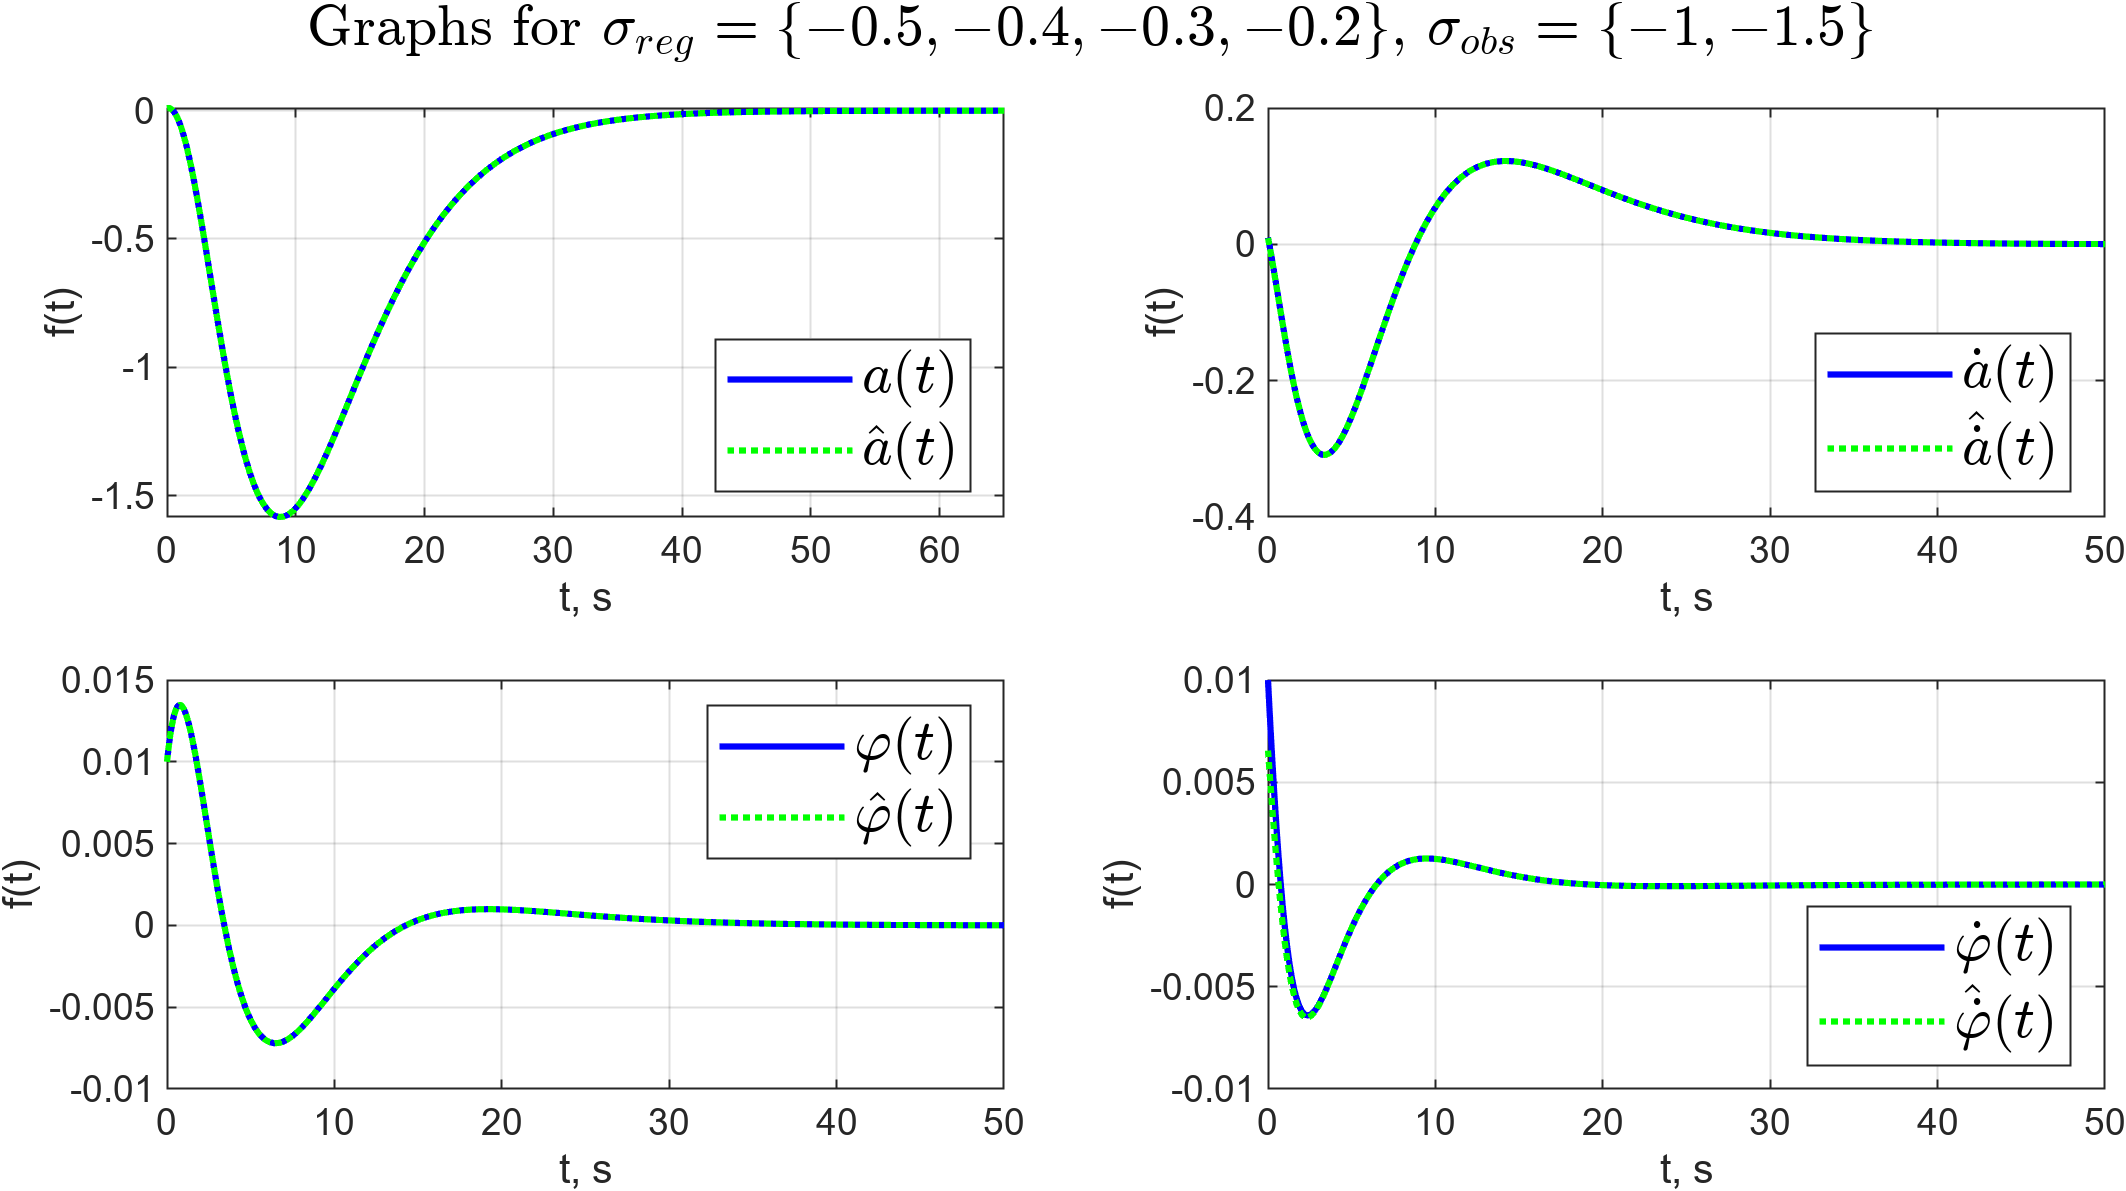
\includegraphics[width=1\linewidth]{pic_fix/3_x_k3l1.png}}
	\caption{Графики векторов состояния системы и наблюдателя для $\sigma_{reg} = \{ -0.5, -0.4, -0.3, -0.2\}$, $\sigma_{obs}= \{-1, -1.5 \}$.}
	\label{3_x_k3l1}
\end{figure}

\begin{figure}[!h]
	\center{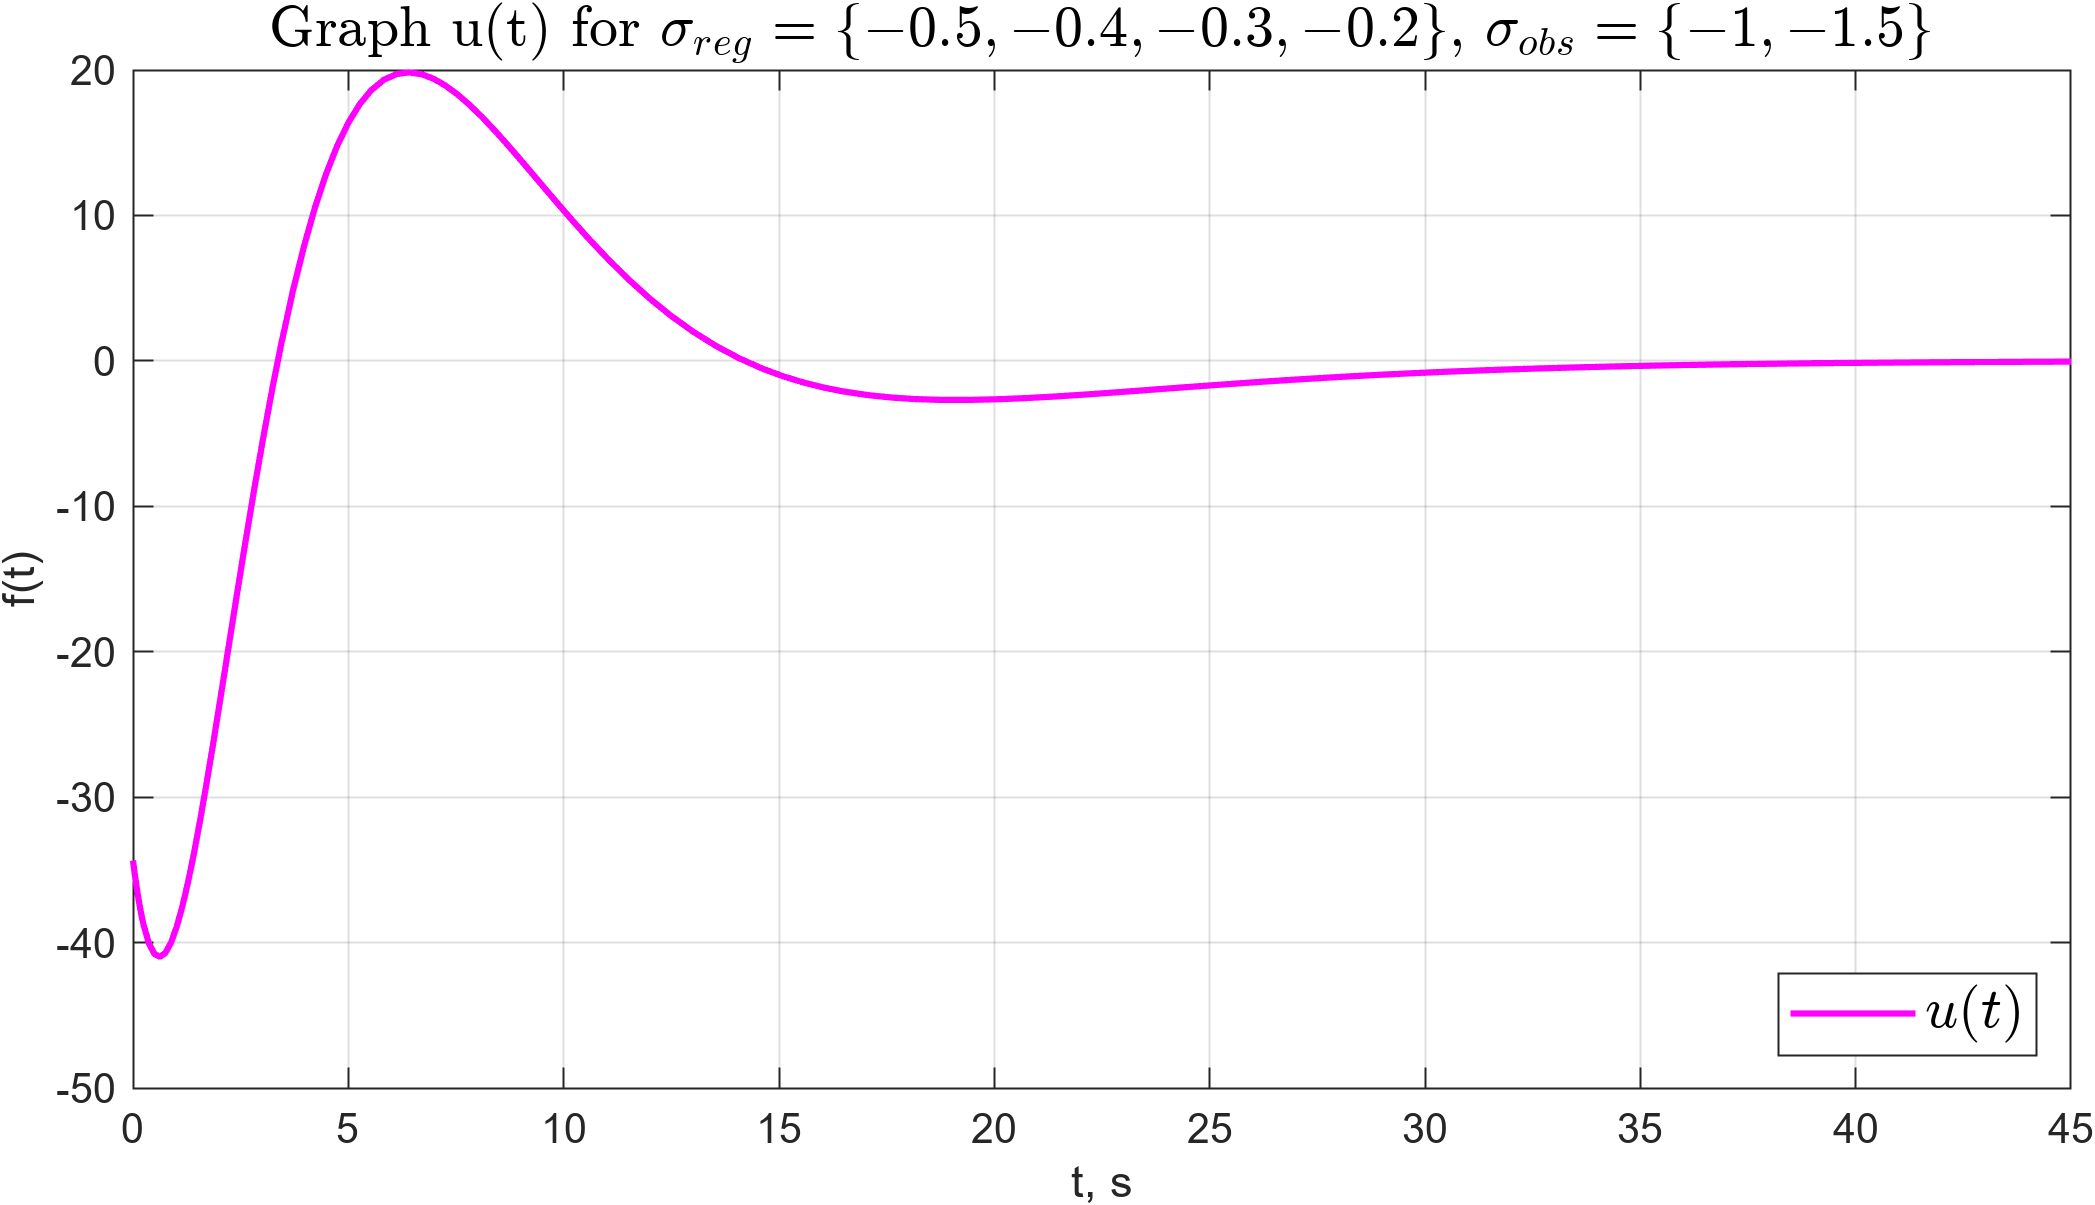
\includegraphics[width=1\linewidth]{pic_fix/3_u_k3l1.png}}
	\caption{График $u(t)$ для $\sigma_{reg} = \{ -0.5, -0.4, -0.3, -0.2\}$, $\sigma_{obs}= \{-1, -1.5 \}$.}
	\label{3_u_k3l1}
\end{figure}

% K1L2

\begin{figure}[!h]
	\center{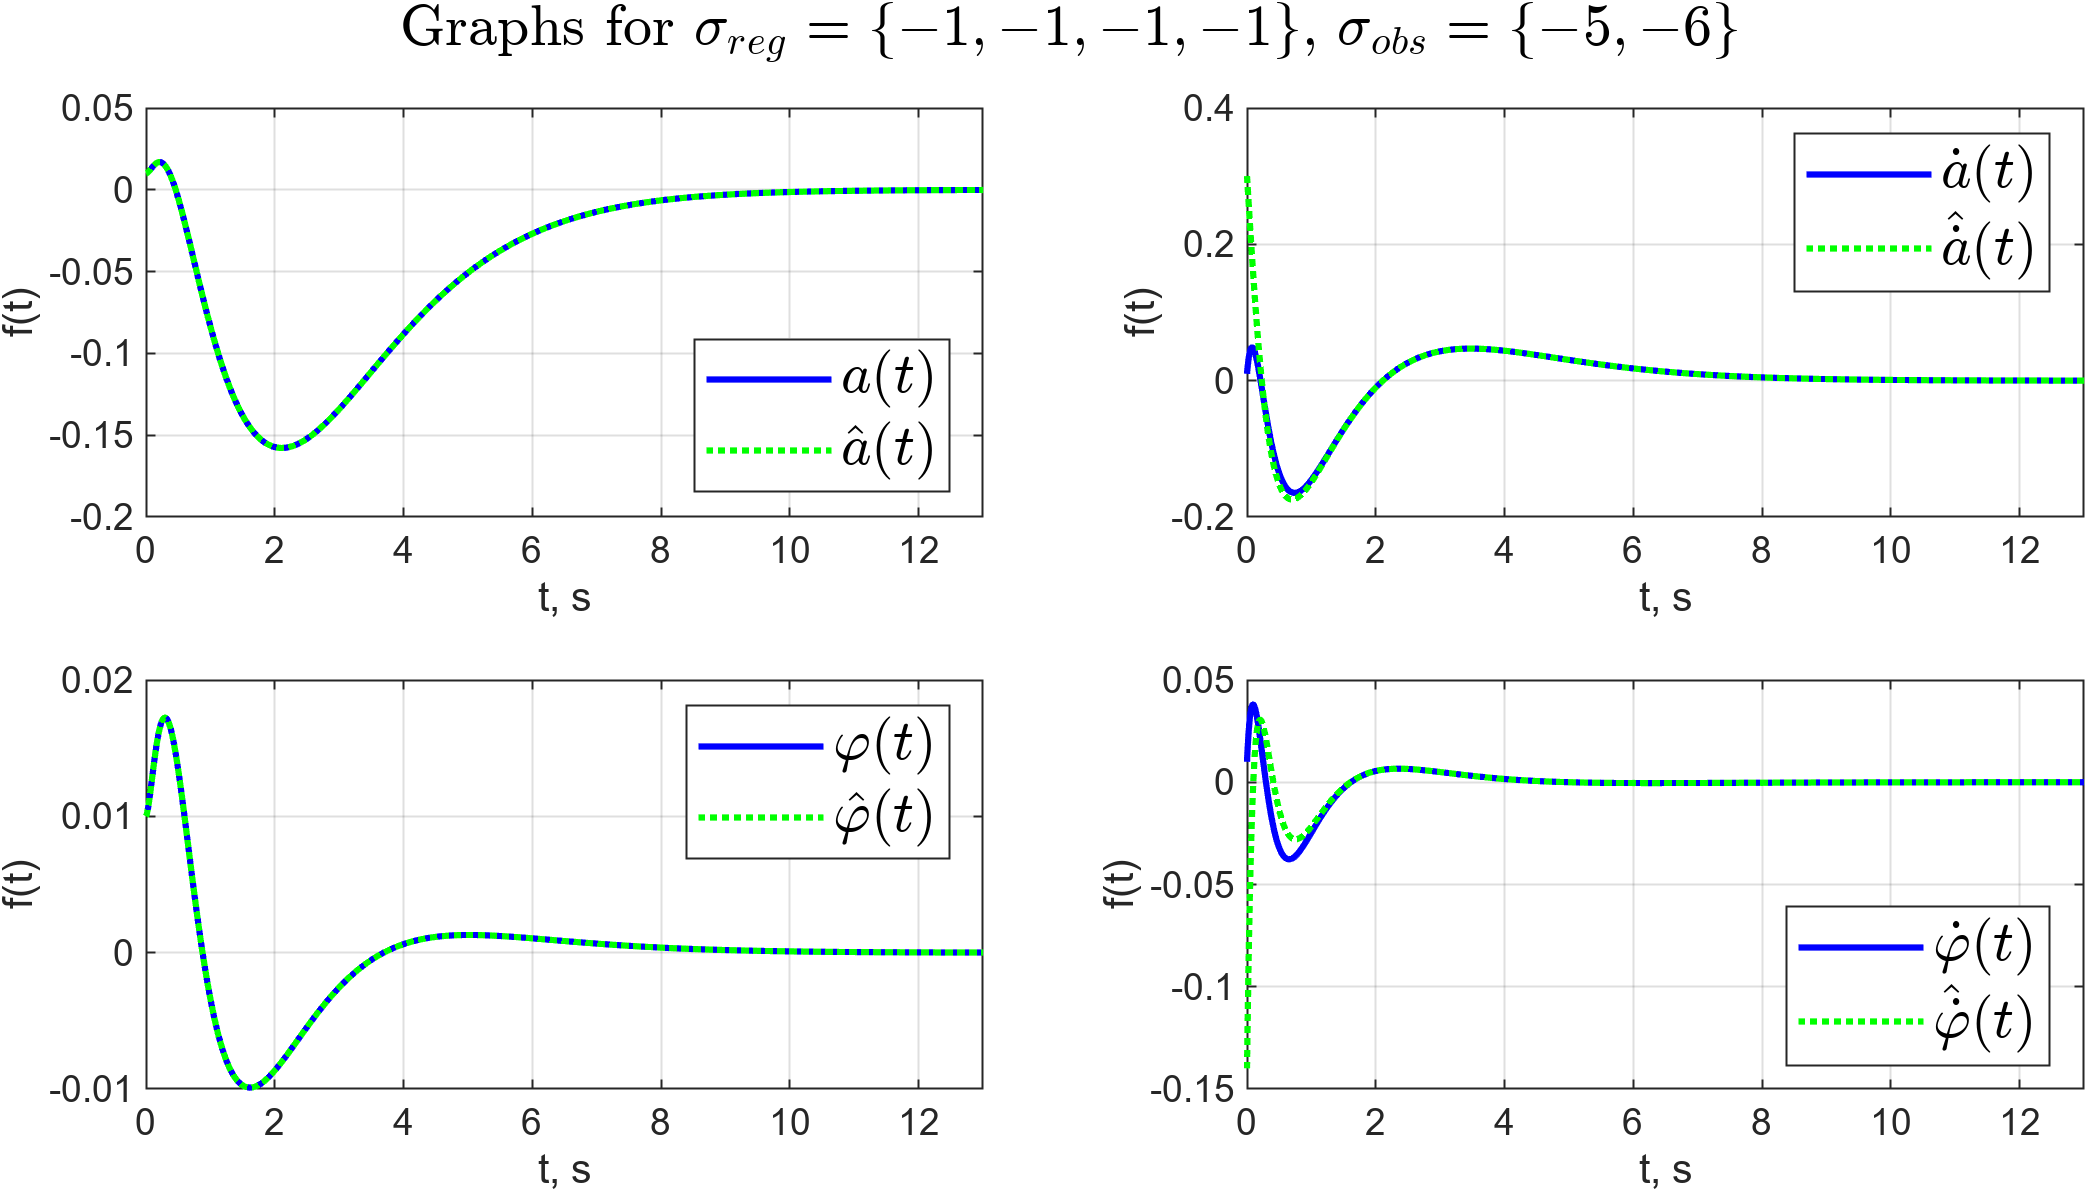
\includegraphics[width=1\linewidth]{pic_fix/3_x_k1l2.png}}
	\caption{Графики векторов состояния системы и наблюдателя для $\sigma_{reg} = \{ -1, -1, -1, -1\}$, $\sigma_{obs}= \{-5, -6 \}$.}
	\label{3_x_k1l2}
\end{figure}

\begin{figure}[!h]
	\center{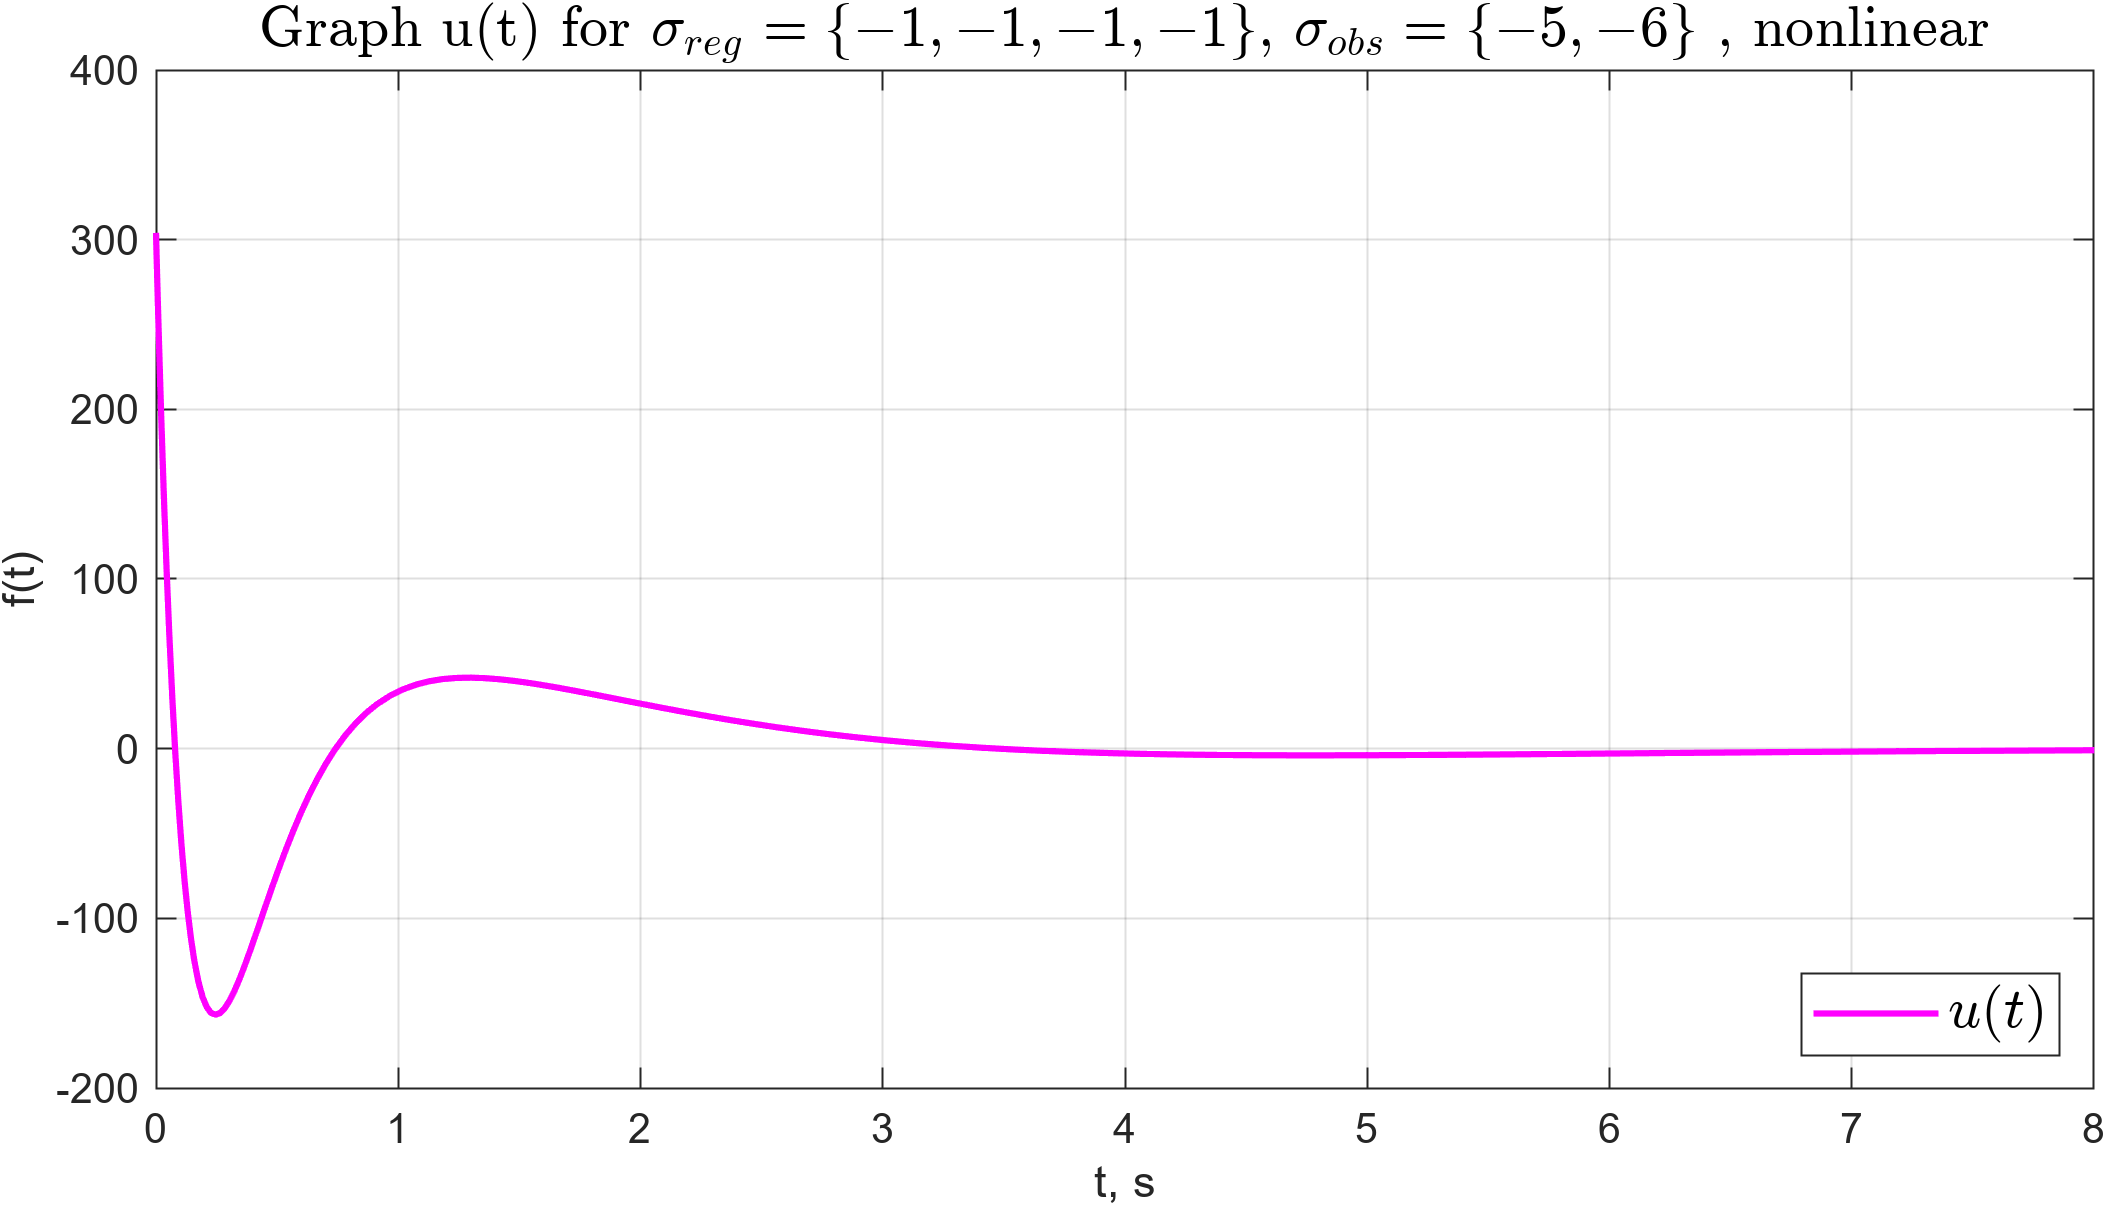
\includegraphics[width=1\linewidth]{pic_fix/3_u_k1l2.png}}
	\caption{График $u(t)$ для $\sigma_{reg} = \{ -1, -1, -1, -1\}$, $\sigma_{obs}= \{-5, -6 \}$.}
	\label{3_u_k1l2}
\end{figure}

% K2L2

\begin{figure}[!h]
	\center{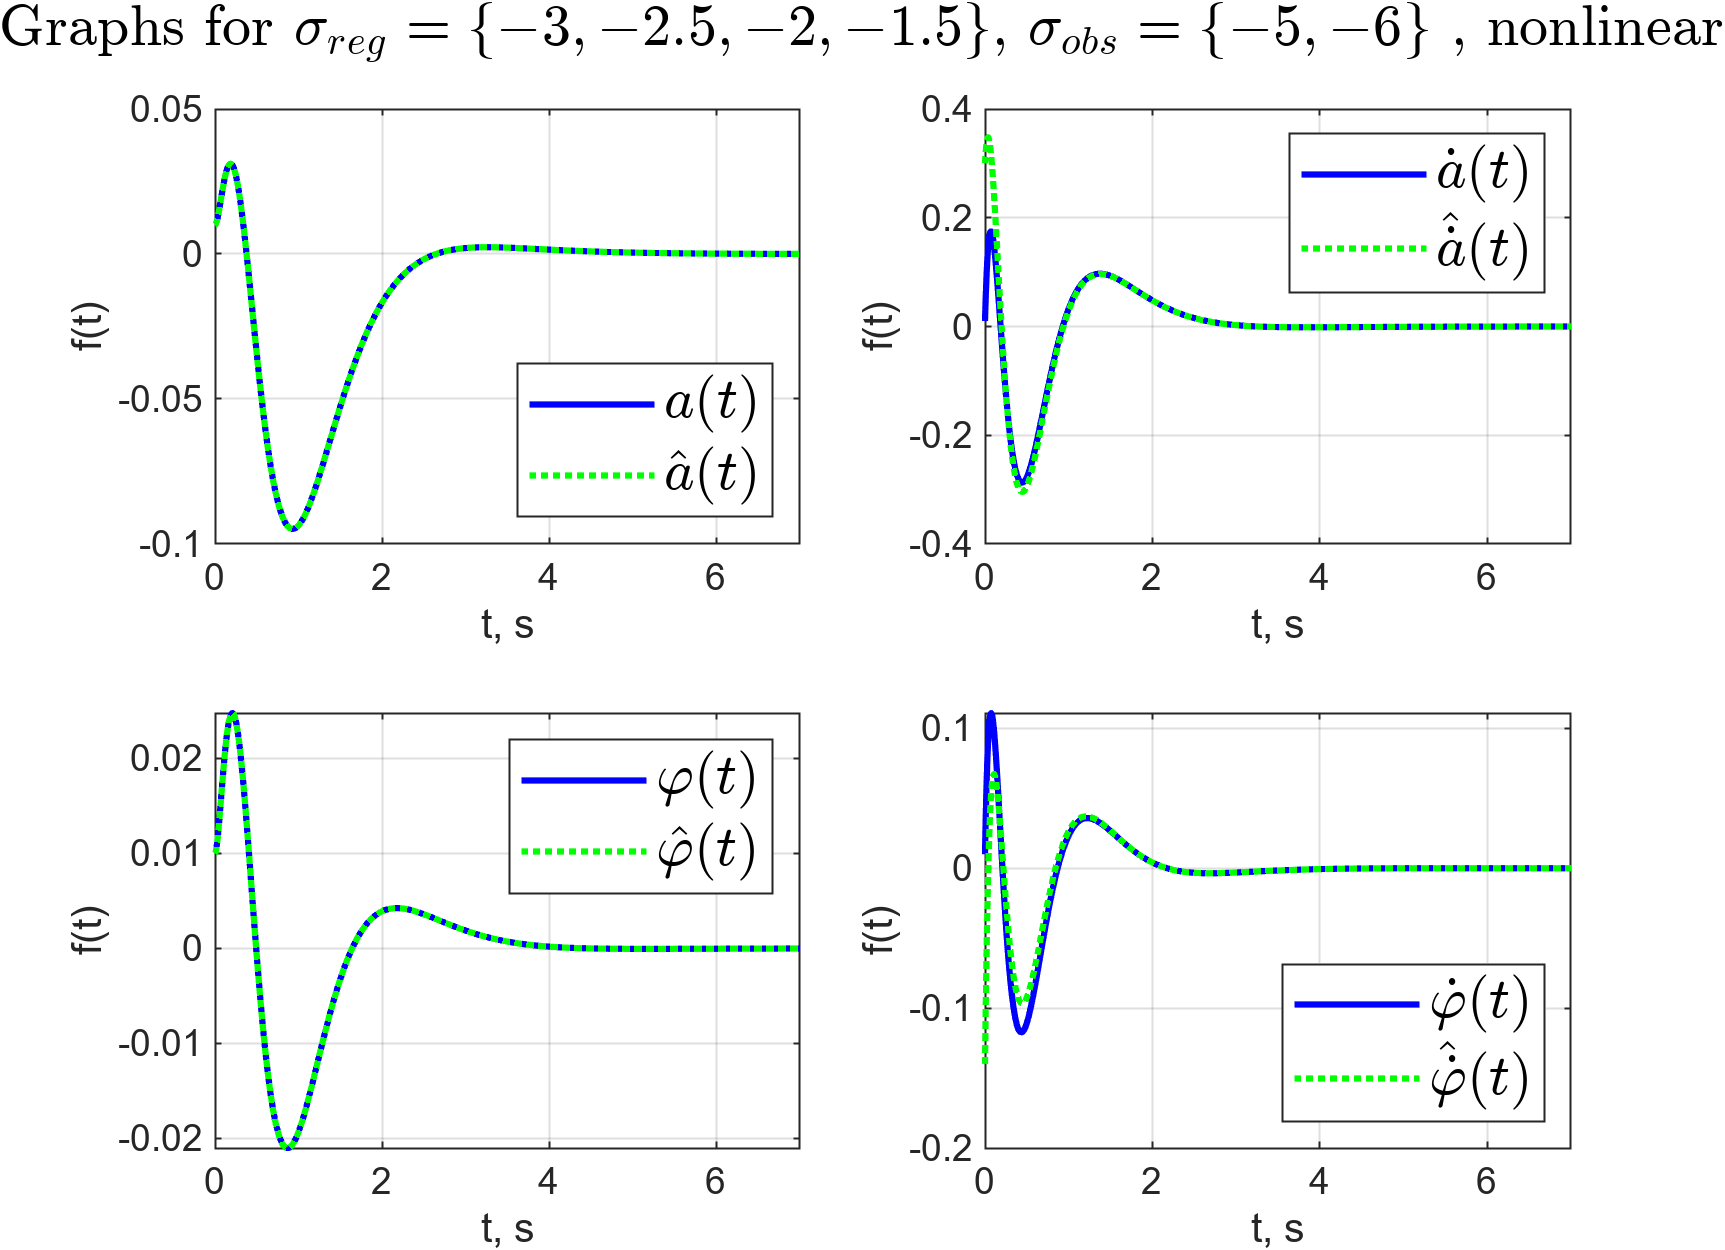
\includegraphics[width=1\linewidth]{pic_fix/3_x_k2l2.png}}
	\caption{Графики векторов состояния системы и наблюдателя для $\sigma_{reg} = \{ -3, -2.5, -2, -1.5\}$, $\sigma_{obs}= \{-5, -6 \}$.}
	\label{3_x_k2l2}
\end{figure}

\begin{figure}[!h]
	\center{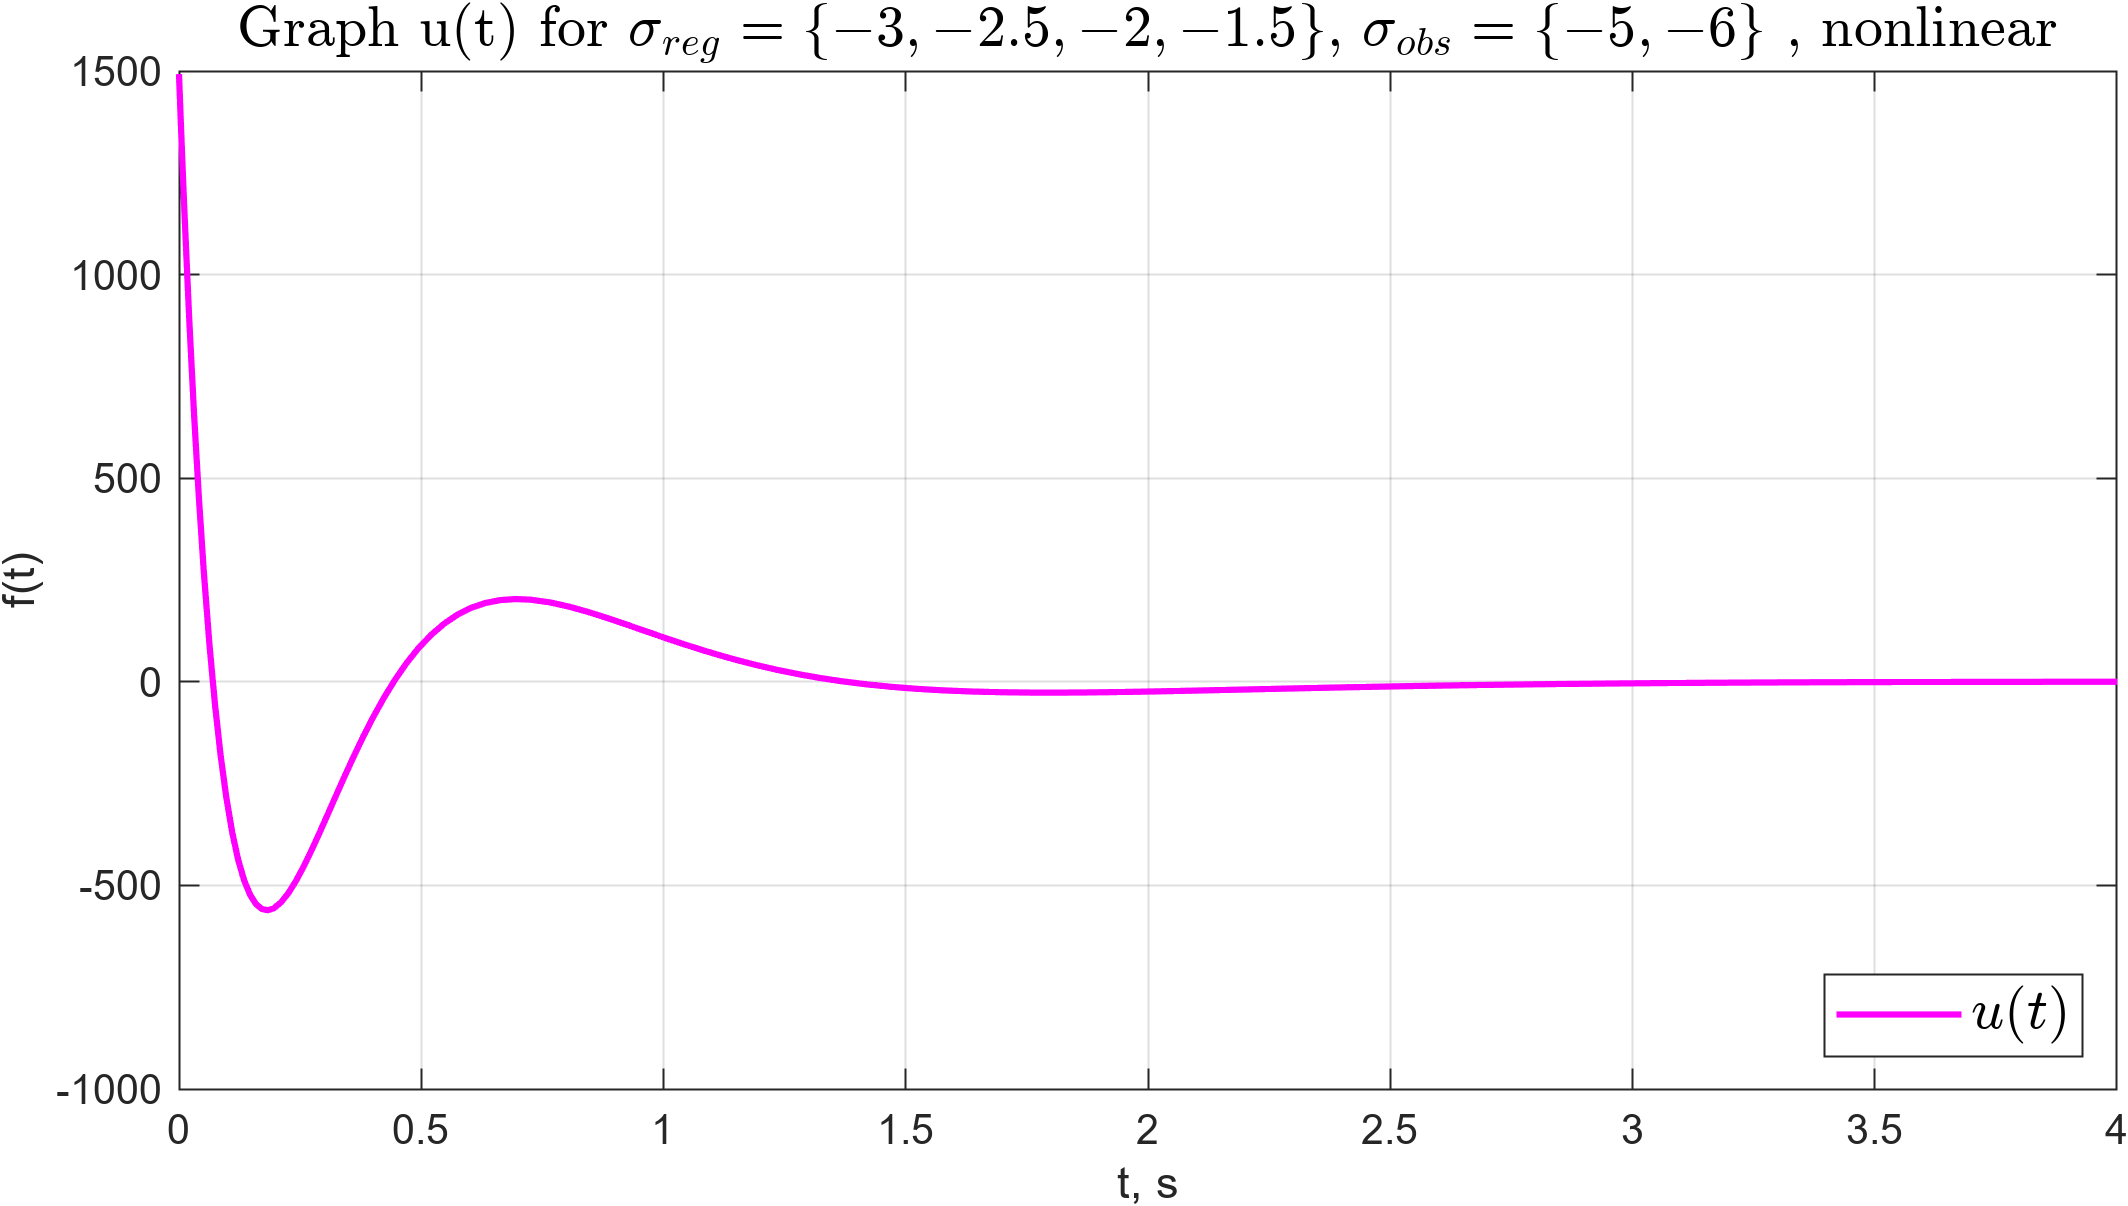
\includegraphics[width=1\linewidth]{pic_fix/3_u_k2l2.png}}
	\caption{График $u(t)$ для $\sigma_{reg} = \{ -3, -2.5, -2, -1.5\}$, $\sigma_{obs}= \{-5, -6 \}$.}
	\label{3_u_k2l2}
\end{figure}


% K3L2
\begin{figure}[!h]
	\center{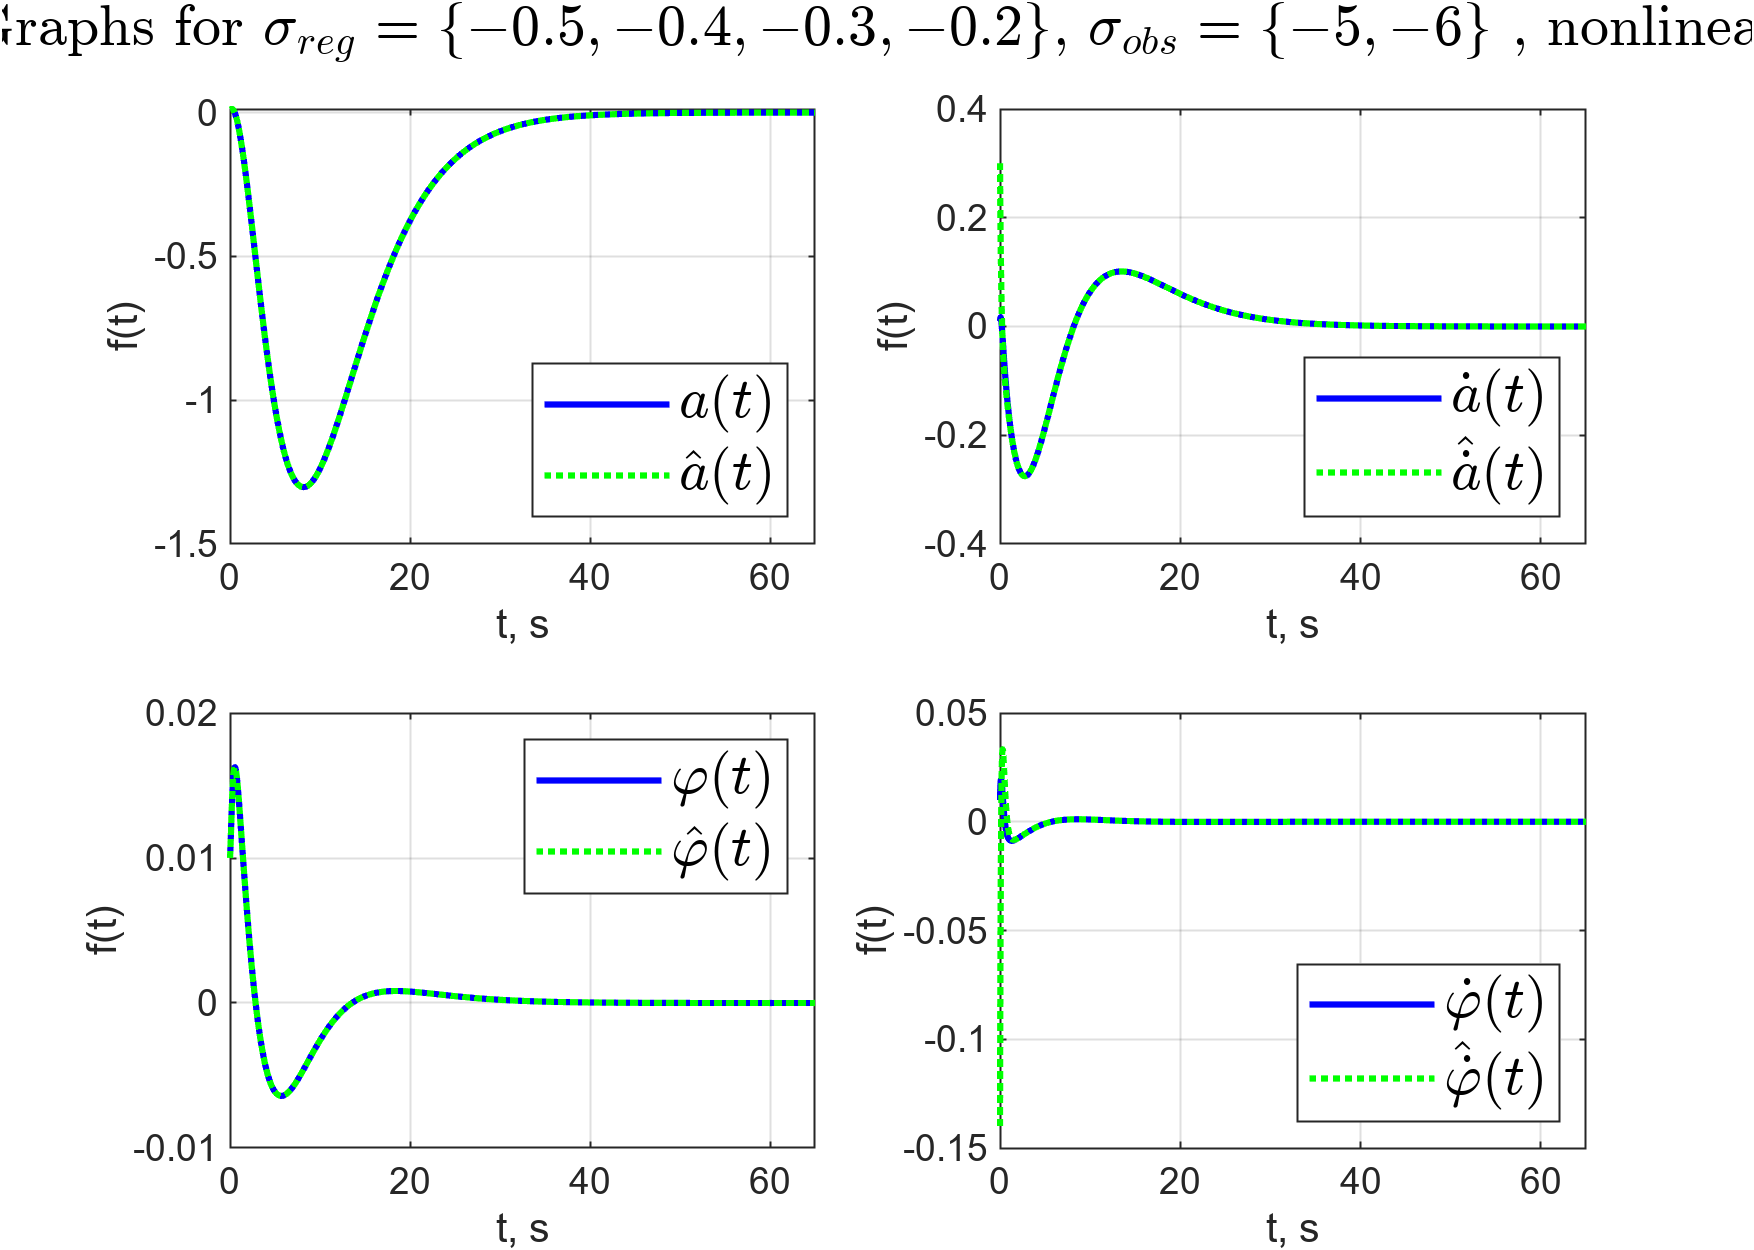
\includegraphics[width=1\linewidth]{pic_fix/3_x_k3l2.png}}
	\caption{Графики векторов состояния системы и наблюдателя для $\sigma_{reg} = \{ -0.5, -0.4, -0.3, -0.2\}$, $\sigma_{obs}= \{-5, -6 \}$.}
	\label{3_x_k3l2}
\end{figure}

\begin{figure}[!h]
	\center{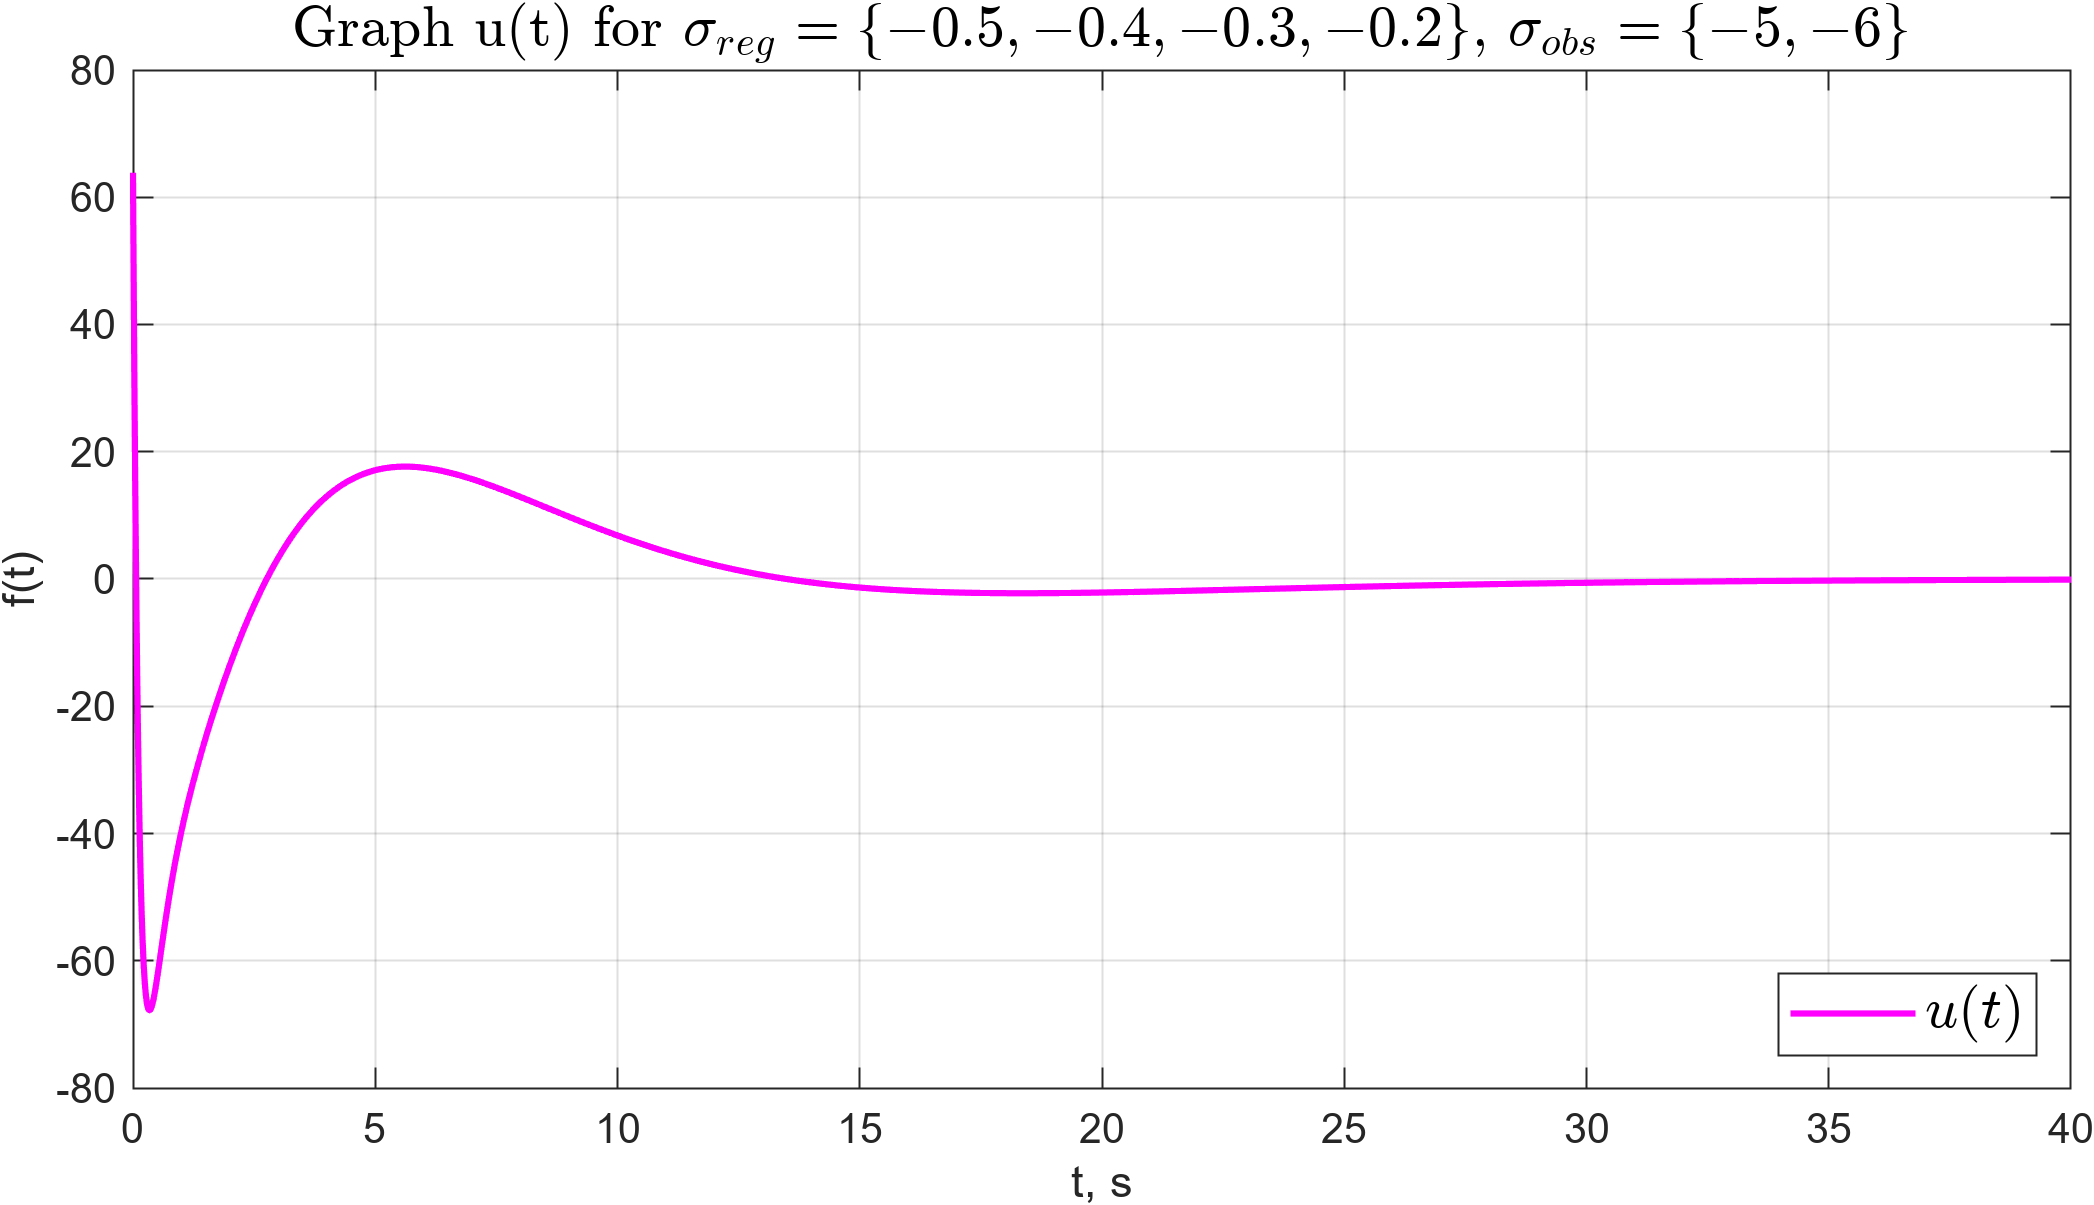
\includegraphics[width=1\linewidth]{pic_fix/3_u_k3l2.png}}
	\caption{График $u(t)$ для $\sigma_{reg} = \{ -0.5, -0.4, -0.3, -0.2\}$, $\sigma_{obs}= \{-5, -6 \}$.}
	\label{3_u_k3l2}
\end{figure}

\endinput